\documentclass[11pt]{article}

\usepackage[utf8]{inputenc}

\usepackage[version=4]{mhchem} %Enables easier chemical reactions

%Format packages
\usepackage[a4paper, left = 3cm, right = 2cm, top = 2.5cm, bottom = 2.5cm]{geometry} %Sets the margin to a nice format
\usepackage[font = small,labelfont=bf]{caption} %Sets the figure captions as bold
\usepackage{setspace}
\usepackage{fancyhdr}
\usepackage{enumitem} %Better enumeration

\onehalfspacing
\setlength{\parindent}{10pt}

%Bibliography packages
\usepackage{csquotes,xpatch}% recommended
\usepackage[backend=biber, style = apa, sorting=none, url=false, alldates=year]{biblatex}
\addbibresource{Preamble/GreenSloth.bib}

%Ref package
\usepackage[]{hyperref}

%Title page
\usepackage{tikz}
\usepackage[dvipsnames]{xcolor}
\usepackage[right]{eurosym}
\usepackage[framemethod=TikZ]{mdframed}

\newcommand{\rate}[1]{v_{\mathrm{#1}}} %\rate takes argument 'x' to put it into v_x in mathmode, while x stays non-italic
\newcommand{\indexni}[2]{#1 _{\mathrm{#2}}} %Create a normal character with a non italic index
\newcommand{\indexnig}[2]{\mathit{#1} _{\mathrm{#2}}} %Create a greek character with a non italic index
\renewcommand{\arraystretch}{1.5}
\newcommand\standardstate{{\circ\kern-0.495em-}}
\newcommand{\cleverref}[3][]{\hyperref[#3]{(see #2~\ref*{#3}#1)}}
\newcommand{\figref}[2][]{\cleverref[#1]{Fig.}{#2}}
\newcommand{\greensloth}[1][GreenSloth]{{\fontfamily{phv}\selectfont\color[HTML]{4c6841}\textbf{#1}}}
\newcommand{\captionprof}[2]{\caption[#1]{\textbf{#1}\\ #2}}

\begin{document}
\selectlanguage{english}
\pagenumbering{roman}

\setlength{\fboxrule}{0.4pt}

\newcounter{theo}[section] \setcounter{theo}{0}
\renewcommand{\thetheo}{\arabic{section}.\arabic{theo}}
\newenvironment{theo}[2][]{%
\refstepcounter{theo}%
\ifstrempty{#1}%
{\mdfsetup{%
frametitle={%
\tikz[baseline=(current bounding box.east),outer sep=0pt]
\node[anchor=east,rectangle,fill=Emerald!20]
{\strut Example~\thetheo};}}
}%
{\mdfsetup{%
frametitle={%
\tikz[baseline=(current bounding box.east),outer sep=0pt]
\node[anchor=east,rectangle,fill=Blue]
{\strut \textcolor{white}{Example~\thetheo:~#1}};}}%
}%
\mdfsetup{innertopmargin=10pt,linecolor=Emerald,%blue!20,%
linewidth=2pt,topline=true,%
frametitleaboveskip=\dimexpr-\ht\strutbox\relax
}
\begin{mdframed}[]\relax%
\label{#2}}{\end{mdframed}}

\thispagestyle{empty}

\vspace*{-3\baselineskip}
\hspace*{0.32\textwidth}\includegraphics[width=0.7\textwidth]{Figures/rwth_jp_computational_life_science_en_rgb.png}\\\vspace{1.5cm}


\vfill


\begin{center}
\Large{Master Thesis}\\
\begin{bfseries}
    \begin{Huge}
        \greensloth{}:\\ A Curated Web Resource for Validating and Comparing Peer-Reviewed Computational Models of Photosynthesis \par
    \end{Huge}
    \LARGE{Elou\"en Corvest}\\[1ex]
\end{bfseries}
\large{submitted to}\\ [1ex]
\large{Computational Life Science, AG Matuszy\'nska\\
Department of Biology, RWTH Aachen University}
\vfill




\begin{large}
    \begin{tabular}{ll}
        Thesis advisor and first examiner: & Prof. Dr. Anna Matuszy\'nska \\
        Second examiner: & Prof. Dr. Oliver Ebenh\"oh \\
        Registration date: & 19.08.2025 \\
        Submission date: & 19.02.2026
    \end{tabular}
\end{large}
\end{center}


\newpage

% Copy below section template for section before TOC
% \newcommand{\secname}{\color{red}REPLACE ME}
% \section*{\secname}
% \addcontentsline{toc}{section}{\secname}
% \input{CHANGE PATH TO SECTION .tex}


\section*{Acknowledgements}
\addcontentsline{toc}{section}{Acknowledgements}

\newpage

\section*{Abstract}
\addcontentsline{toc}{section}{Abstract}

\newpage

\tableofcontents

\newpage

\printglossary[type=abbreviations, title=Acronyms]
\printglossary[type=variable]

\newpage

\addcontentsline{toc}{section}{List of Visualisations}

\lstlistoflistings
\addcontentsline{toc}{subsection}{\lstlistlistingname}

\listoffigures
\addcontentsline{toc}{subsection}{\listfigurename}

\listoftables
\addcontentsline{toc}{subsection}{\listtablename}

\newcounter{romannumbers}
\setcounter{romannumbers}{\arabic{page}}
\newpage

\pagenumbering{arabic}

% Copy the following to create a new section
% \newcommand{\secname}{\color{red}REPLACE ME}
% \section{\secname}
% \input{CHANGE PATH TO SECTION .tex}
% \newpage

\section{Introduction}
\subsection{Preamble}

Photosynthesis is a fundamental process of the very existence of life on Earth~\cite{stirbetPhotosynthesisBasicsHistory2020, janssenPhotosynthesisForefrontSustainable2014,johnsonPhotosynthesis2016}. It provides the starting block for the food chain, and is directly responsible for the oxygen production that lead to the ozone layer. Additionally, it also proves to be a key player in human's more complex lives, as for example, around \qty{82}{\percent} of the world's primary energy consumption is still based on fossil fuels~\cite{FossilFuelShare}, which in turn are mostly made up of dead organic matter of photosynthetic organisms~\cite{pisupadtiFuelChemistry2003}. Therefore, photosynthesis has been a vital part of scientific research for centuries.

The basic principles of photosynthesis have been known since the 18\textsuperscript{th} century~\cite{ingenhouszExperimentsVegetablesDiscovering1779}, giving rise to advanced techniques to study the process in more detail. A key reason for this strive to understand photosynthesis is the potential to use it as a key way to increase crop yield~\cite{murchieAgricultureNewChallenges2009}. While there has been ground-breaking discoveries done in the past, that have introduced the Green Revolution, those methods have long reached a plateau in terms of improvement~\cite{longCanImprovementPhotosynthesis2006}. Therefore, there is a need to find new ways to change photosynthesis, however, this time in a new light. Instead of focusing on what comes out of experiments, a view more directed into the inner workings of photosynthesis is needed. To be able to change a process, it is necessary to understand it. This is where mathematical modelling comes in.

Mathematical modelling has been a staple of sciences for centuries~\cite{banerjeeMathematicalModelingModels2021}. From using simple geometry for calculating the distance to the sun, to simulate neutron transport in nuclear fission~\cite{demaziereModellingNuclearReactor2020}. This method has not gone unnoticed in the world of photosynthesis research, and has given rise to a large variety of models. Some focus on specific parts of the process~\cite{liImpactIonFluxes2021,matuszynskaMathematicalModelNonphotochemical2016}, some on specific ways the photosynthesis machinery reacts to the environment~\cite{fuenteMathematicalModelSimulate2024}. Some depict the process in a very simplified manner~\cite{farquharBiochemicalModelPhotosynthetic1980,voncaemmererSteadystateModelsPhotosynthesis2013,lochockiWidelyUsedVariants2025a}, while others try to capture the process in all its complexity~\cite{zhuEphotosynthesisComprehensiveDynamic2013}. There are many different ways mathematical modelling has been used to understand photosynthesis, which can be seen by still growing influx of new publications over the years'~\figref{fig:intro-photosynthesis-models}.

\begin{figure}
    \centering
    \includegraphics[width=\textwidth]{Figures/bibsearch.pdf}
    \captionprof{Results of a bibliography search for photosynthesis models.}{A basic bibliography search was done to find the publications with the words "photosynthesis" and "model" in the title, between 1970 and 2025. On the left, the cumulative number of publications over the years is shown, with the new publication of the respective year are shown in green. On the right, the number of new publications per Year is shown. The two colors were chosen to be easily distinguishable and do not have any specific meaning. The data was obtained from the Web of Science database on the 14\textsuperscript{th} of February 2026. The query used was "TI=(("photosynthesis" OR "photosynthetic") AND ("model*" OR "modelling" OR "modeling" OR "simulation" OR "representation"))", and can be found here: \url{https://www.webofscience.com/wos/woscc/summary/0b793bdb-ab8b-456e-a5fb-085fc470f5a2-019f07a73b/relevance/1}}
    \label{fig:intro-photosynthesis-models}
\end{figure}

With all these different models and ways to see photosynthesis, one cannot point to a single one as the "best" one. Each model has its own advantages and disadvantages, often tailored to answer specific questions. On top of that, many models work on top of each other, taking inspiration or even entire structures. It may be done to improve a model, or to make it more accessible to a different audience. Sometimes, it may also be used to answer a different scientific question, that may not have been the intention of the original model. A strong example of this, is the \gls{fvcb} model~\cite{farquharBiochemicalModelPhotosynthetic1980}, a simple model that describes the \gls{A} as a function of \gls{vc}, \gls{vo}, and \gls{rlight}. Even through its simplicity, it has amassed a large amount of citations, also in non-modelling branches. The main field using the \gls{fvcb} model are obviously the plant sciences, but it has found its way into other fields, such as ecology, forestry, and more~\figref{fig:intro-fvcb-cits}. It has become so popular in fact, that many different versions have come to fruition. Some that take the original model as a starting point and add on more complexity~\cite{voncaemmererSteadystateModelsPhotosynthesis2013,bellasioGeneralisedDynamicModel2019}, or others that use it solely as a readout for \gls{A}~\cite{zhuEphotosynthesisComprehensiveDynamic2013}. It has become so popular in fact, that even misinterpretations of the original model are ingrained in photosynthesis modelling~\cite{lochockiWidelyUsedVariants2025a}.

\begin{figure}
    \centering
    \includegraphics[width=0.3\textwidth]{Figures/fvcb_analyse.pdf}
    \captionprof{Number of citations of the original \glsentryshort{fvcb} publication separated in categories.}{The citations of the original \glsentryfull{fvcb} model publication~\cite{farquharBiochemicalModelPhotosynthetic1980} were obtained from the Web of Science database on the 16\textsuperscript{th} of February 2026. These citations were separated into categories based on the Web of Science categories of the citing publication. The five most populated categories were taken, while the others were grouped into "Others".}
    \label{fig:intro-fvcb-cits}
\end{figure}

While this rise in popularity of photosynthesis models brings, on the one hand, more and more tools to understand photosynthesis, it also brings a lot of confusion. Models differing in their concept, basing their work on different assumptions, and sometimes even misinterpreting starting blocks, can make it hard to see through the web of models. While it is not fair, to say that the waters of photosynthesis modelling are polluted, it is fair to say that there exists a problem of clarity. This is not only a problem for newcomers to the field, but also experienced researchers, who may find it hard to keep up with the ever-growing number of models. This problem of clarity, has already come into focus of the scientific community and it is not limited to photosynthesis modelling. Therefore, some proposed solutions already exist. Three key problems have been identified and solutions proposed: \hyperref[sec:intro-model-creation]{1) Model Creation}, \hyperref[sec:intro-model-presentation]{2) Model Presentation}, and \hyperref[sec:intro-model-sharing]{3) Model Sharing}. While all three are very intertwined, a clear distinction can be made between them.

\subsection{Current Problems and Solutions}

\subsubsection{Model Creation}\label{sec:intro-model-creation}

Model Creation, comes in many different ways, therefore the transparency of the process is vital. Some may be written from scratch using Python or Matlab, while others may be built using more specialized software for modelling, such as \verb|mxlpy|~\cite{vanaalstMxlPyPythonPackage2025}, \verb|COPASI|~\cite{hoopsCOPASICOmplexPAthway2006}, or \verb|Tellurium|~\cite{choiTelluriumExtensiblePythonbased2018}. Whatever the method used, one problem persists throughout all of them: the annotation and documentation of the model is based on the author. This means, that great care needs to be taken to make sure that the model is reproducible and understandable by others. This is not only a problem of the model description, but also of the code itself. As computational methods adapt and evolve, the code may become outdated and hard to read. There have been attempts to solve this problem, one of the most notable ones being the \gls{sbml}~\cite{huckaSystemsBiologyMarkup2003}. 

It breaks down the concept of a model into its most basic components, such as the compartment, species, reaction, and so on~\cite{huckaSystemsBiologyMarkup2003}. This creates a schematic overview of the model system which makes it much easier to be understood by different languages. Just as a schematic overview of photosynthesis is used in school books to explain that \gls{o2} is produced from water and not \gls{co2}, \gls{sbml} provides a schematic overview of the model so different software can understand it better. This simplification of complex systems

It does not provide ways to use the model, but it does provide a way to represent it in a way, that many different software can read it. Just like a schematic overview of photosynthesis is used in school books to explain that \gls{o2} is produced from water and not \gls{co2}, \gls{sbml} provides a schematic overview of the model so different software can understand it better.


\subsubsection{Model Presentation}\label{sec:intro-model-presentation}

\subsubsection{Model Sharing}\label{sec:intro-model-sharing}

\newpage

\section{Material and Methods}
\subsection{Models}

To make a good demonstration of the capabilities of \greensloth{}, five kinetic \gls{ode} models of photosynthesis have been chosen to take part in this thesis. These five models, while all showing photosynthesis, vary in their complexity and execution. Some are based on each other, while others stand alone. In the following, a brief description of each model is given. These short summaries are the ones used on the \greensloth{} website. Additionally, the models are validated by trying to recreate the figures of the original publication, as close as possible. Due to permissions and licensing issues, the original figures will not be present in this thesis nor \greensloth{}. However, the publication is rightfully cited and so, the user can easily find the original figures, if they have access to the publication.

\subsubsection{Bellasio2019}
The Bellasio2019~\cite{bellasioGeneralisedDynamicModel2019} model is a generalized C\textsubscript{3} leaf-photosynthesis model, that includes simplified representations of the light and dark reactions and a stomatal behavior submodule. A lot of its implementation is based on past work by the same author and is mainly inspired by the common \gls{fvcb} model. The light reactions are modified from Yin et al. (2004) and include the potential rates of ATP and NADPH production based on light intensity. This model has been created with the simple user in mind, and the author has made an effort to show its simplicity, by giving access to a Microsoft Excel Workbook containing the entire model. To showcase the model's capabilities, the author creates common steady-state carbon assimilation curves, against intercellular CO2 concentration and light intensity, and compares them to experimental data from the literature. As many models of photosynthesis rely on purely stead-state assumptions, this model is also validated in dynamic conditions, showing for example the response of the model to a fluctuation of ambient oxygen concentration.

This model was created to stay as simple as possible, while still being able to accurately represent the main features of C\textsubscript{3} photosynthesis. As such, it can be used as a base for more complex models, or as a starting block in larger models of plant physiology. While giving access to the entire model in an Excel Workbook format is transparent and great, the execution of said practice has been inefficient in this instance. The entire mathematical description of the model is also given in the Appendix of the publication, however there are missing or different equations between the publication and the Excel Workbook, which can lead to confusion. On top of that, the simulation protocols used for each figure are only given in small details, which leads to further confusion when trying to reproduce the results and see which equations are correct or not.

\subsubsection{Fuente2024}
The Fuente2024~\cite{fuenteMathematicalModelSimulate2024} model is a kinetic model of photosynthesis that is based on Occam's razor, aiming to provide the minimal complexity to describe the core processes of this model. In this case, the model focuses on the dynamic light oscillation and its responses on the photosynthetic machinery. It focuses only on the light-dependent reactions, including simplified versions of photosystem II, photosystem I, the Plastoquinone pool, and proton and ATP concentration in the lumen and stroma. On top of that, it shows the activation of non-photochemical quenching (NPQ), the dynamics of chlorophyll fluorescence, and the rate of oxygen evolution.
                     
The model includes the oscillating light intensity as a sinusoidal function, where the amplitude and frequency are adjustable parameters. To allow for easier comparison to other models, that often see light intensity as a constant value, the oscillation is defined around a base light intensity. However, the strength of having light with a specific frequency lies in the additional information and therefore analysis possibilities that can be performed. In this case, the model is used to create Bode plots of the response of fluorescence to light oscillations and comparing these results to experimental data from \gls{chlamydomonas}.

This simple model stays true to its name and the authors aim to provide a base model that can be easily extended, while still showing a new approach to photosynthesis modelling. Their work shows that even with a simple model, new insights can be gained by using dynamic light protocols, which may have been overlooked in traditional steady-state models. To further extend the usability of the model, the authors provide a detailed notebook written in the Wolfram language, which also shows how to recreate some of the publication's figures.

\subsubsection{Li2021}

\subsubsection{Matuszynska2016}
The Matuszynska2016~\cite{matuszynskaMathematicalModelNonphotochemical2016} model, a small kinetic model, was developed to delve deeper into the effect of light memory caused by non-photochemical quenching. The systematic investigation of the Xanthophyll cycle, a combination of the pigments of violaxanthin, antheraxanthin, and zeaxanthin, sparked a series of experiments to determine whether plant light memory can be detected in a timescale of minutes to hours through pulse amplitude modulated chlorophyll fluorescence. The model was then created based on these experimental results, providing a comprehensive description of \gls{npq} dynamics and the short-term memory of the \gls{arabidopsis} plant.

To keep the model as simple as possible, several processes not directly linked to \gls{npq} have been simplified to create a dynamic ODE system consisting only of 6 different compounds. With these simplifications, the authors could fulfil an additional goal: to make a general framework that is not specific to one model organism.

To demonstrate the adaptability of their model, the authors took their calibrated \gls{arabidopsis} model and successfully applied it to the non-model organism \gls{epipremnum}. This adaptation allowed them to simulate realistic fluorescence measurements and replicate all the key features of chlorophyll induction, showcasing the model's versatility and potential for use in a variety of organisms.

\subsubsection{Saadat2021}
The Saadat2021~\cite{saadatComputationalAnalysisAlternative2021} model builds upon previous models, particularly the Matuszynska2019 model, by incorporating and modifying various reactions and aspects of photosynthesis. Overall, the model can be divided into three modules: the ascorbate-glutathione cycle, the \gls{cbb} cycle and thioredoxin reductase-regulated reactions, and the \gls{petc}.

The model is primarily used to investigate the electron flows around PSI and their relevance to photosynthetic efficiency. Several different analyses have been conducted to validate the model in both steady-state and dynamic environment conditions. The most interesting is the direct comparison of a knockout mutant of the protein PGR5. This protein is known to catalyse the reduction of plastoquinone by ferredoxin. The results of this comparison align with experimental values, which are, however, not presented in the publication but are referenced. Additionally, it is noted that the results should not be interpreted as accurate quantitative data, but rather as a proof of concept for the model.

Overall, the model has one advantage over other photosynthesis models, as it also highlights the importance of other electron flows, not just the \gls{petc}. Additionally, not only are the authors open about the model's flaws, but they are also insistent on making their code and analyses available on GitHub. Therefore, this model serves as a good stepping stone for more complex models that aim to incorporate aspects of photosynthesis, which are often simplified in other models.

\subsection{Model Demonstrations}\label{sec:model-demonstrations}

\subsubsection{Daylight Simulation}
The \gls{ppfd} data in a 1-minute resolution used for the daylight simulation demonstration is taken from \gls{neon} at the KONZ site, located in Kansas, USA (39.10077, -96.56307)~\cite{nationalecologicalobservatorynetworkneonPhotosyntheticallyActiveRadiation2023}, using the \verb|neonutilities| package~\cite{lunchNeonutilitiesPackageAccessing}. As only a day is shown in the simulation, only data from the 19th of June 2023 is taken into account. To limit the data to only the part of day that has sunlight, and a decent amount at that, the data is filtered to only include data that has a \gls{ppfd} value higher and equal than \qty{40}{\micro\mol\per\square\meter\per\second}. This threshold is chosen as it has shown to allow most models to still simulate the photosynthetic machinery, while still being a decent representation of the actual daylight conditions. The filtered data is then used as an input for the \gls{ppfd} parameter in the daylight simulation demonstration for every model. The protocol is constructed by simulating each point of \gls{ppfd} data for 60 seconds. Three different outputs are shown in this demonstration: the \gls{vc}, the \gls{atp} and \gls{nadph} ratio, and the \gls{F} yield. If these outputs are not available in the model at hand, the plot is still displayed with the corresponding y-axis label, struck through.

\subsubsection{FvCB Add-on}
The basis of the \gls{fvcb} add-on demonstration is based on the min-$W$ variant. If the supplied model already has a \gls{A}, then a generic FvCB simulation is done and compared to the results from von Caemmerer (2013)~\cite{voncaemmererSteadystateModelsPhotosynthesis2013}. If there is no available instance of \gls{A}, the two main and mandatory connection points for the add-on are the \gls{vc} and a quantity that represents \gls{co2}. If these two connection points are not available in the model, the simulation will not run, and only the general \gls{fvcb} output will be shown.

The \gls{vc} needs to be in a unit of \unit{\micro\mole\per\square\meter\per\second}. To convert from a concentration per time unit, the space that the stroma occupies in the chloroplast based on the leaf volume needs to be used. The value taken for this add-on was taken from Laisk et al. (2006)~\cite{laiskC3PhotosynthesisSilico2007}, where it was estimated and set to \qty{0.0112}{\liter\per\square\meter}.

As the \gls{fvcb} model requires a partial pressure of \gls{co2}, specifically the \gls{ci}, this quantity can also be given to the add-on if available in the model at hand. If it is not given, but the \gls{co2} is, a conversion using Henry's law is done to convert the concentration of \gls{co2} into a partial pressure. The default Henry's law constant used for this conversion is \qty{3.4e-5}{\milli\molar\per\micro\bar}~\cite{sanderCompilationHenrysLaw2023}, however, the law constant can also be supplied, when it is a part of the model.

With these two quantities given in the correct format, the \gls{fvcb} add-on can be added to any kinetic \gls{ode} model of photosynthesis. To finally create the representation of \gls{A}, the add-on includes the \gls{gammastar} and \gls{rlight}, \qty{38.6}{\micro\bar} and \qty{1}{\micro\mol\per\square\meter\per\second}, respectively, if not given by the model. With all of these quantities included in the model, the \gls{A} can be calculated~\cleverref[]{Equation}{eq:fvcb} and shown in the demonstration plot with a generic \gls{fvcb} simulation using parameters taken from von Caemmerer (2013)~\cite{voncaemmererSteadystateModelsPhotosynthesis2013}.

\begin{equation}
  \label{eq:fvcb}
  \glsxtrshort{A} = \glsxtrshort{vc} \cdot \left( 1 - \frac{\glsxtrshort{gammastar}}{\glsxtrshort{ci}} \right) - \glsxtrshort{rlight}
\end{equation}

\subsubsection{Standard PAM Simulation}
The standard \gls{pam} simulation demonstration uses a generic protocol that does not reflect actual experiments, but are in the same spirit as true experimental work. Prior to the actual protocol, the simulation of the model is done under dark conditions for \qty{30}{\min}. Then the actual protocol consists of 22 periods of a length of \qty{2}{min}, which start with the specific light intensity of that period and ends with a saturating pulse of \qty{3000}{\micro\mol\per\square\meter\per\second} for \qty{0.8}{\second}. The first two periods are in dark conditions, followed by 10 periods of actinic light of \qty{1000}{\micro\mol\per\square\meter\per\second} and finishes with 10 periods of dark conditions again. The dark condition is set to \qty{40}{\micro\mol\per\square\meter\per\second}, as it has been found that many models are not capable of simulating actual zero light conditions.

With this protocol, the simulation of the model is run and the \gls{F} and \gls{npq} is shown in the demonstration plot. If \gls{F} is not present in the model, the corresponding plot is still displayed with the y-axis label struck through. If \gls{npq} is not available, but \gls{F} is, it is calculated by using \gls{Fm}~\cleverref[]{Equation}{eq:npq}.
 
\begin{equation}
  \label{eq:npq}
  \glsxtrshort{npq}(t) = \frac{\glsxtrshort{Fm}(t=0) - \glsxtrshort{Fm}(t=t)}{\glsxtrshort{Fm}(t=t)}
\end{equation}

\gls{Fm} is extracted by using the simulated \gls{F} values at the time points where the saturating pulses are applied. To be sure that the actual \gls{Fm} is found, an interval between the two saturating pulses is taken, and the maximum value in that interval is used as \gls{Fm}. Most of the time this value is correct, but for full transparency, these values are plotted as triangles on the \gls{F} plot, additionally to the \gls{npq}.
\subsubsection{MCA of Photosynthesis}
The \gls{mca} demonstration limits its analysis to variables and fluxes that are deemed integral parts of photosynthesis. The variables to be given should account for a representation of \gls{pga}, \gls{rubp}, \gls{pq_ox}, \gls{pc_ox}, \gls{atp}, and \gls{nadph}. The rates should include the \gls{vc}, \gls{vpsii}, \gls{vpsi}, \gls{vb6f}, and \gls{vatp}. The parameters analyzed are supposed to be the control coefficients of each prior mentioned rate, and therefore the \gls{mca} simulations are run to steady-state. Each parameter is displaced by $\pm \ 0.01 \%$ and the results are put into two separate heatmaps, one for the variables and one for the fluxes. If any of the prior mentioned variables or rates are not available in the model, the corresponding row and column in the heatmaps are still displayed, but white and with less opacity.

\subsubsection{Fitting of NPQ}
The fitting demonstration uses experimental data taken from von Bismarck (2022)~\cite{vonbismarckLightAcclimationInteracts2023}. The data consists of measurements of \gls{F}, \gls{Fm}, and \gls{npq} calculated~\cleverref[]{Equation}{eq:npq} under different light intensities, following a \gls{pam} protocol after a dark adaptation period of \qty{5}{\min}. The data was taken with Maxi Imaging-PAM (Walz, Germany) using Col-0 \gls{arabidopsis} plants and as no details were given, the default settings of the machine are taken. That means, that each saturating pulse is \qty{5000}{\micro\mol\per\square\meter\per\second} for \qty{720}{\milli\second}. Each period consists of a simulation of a specific light intensity and finishes with a saturating pulse, together lasting approximately \qty{1}{\min}. There are four different sections during this \gls{pam} protocol. Starting with one dark period with a light intensity of \qty{0}{\micro\mol\per\square\meter\per\second}, followed by 10 high actinic light periods of \qty{903}{\micro\mol\per\square\meter\per\second} then dropping the actinic light to \qty{90}{\micro\mol\per\square\meter\per\second}, also for 10 periods, then again 5 dark periods to finish the protocol.

The protocol used for the simulation is based on the actual data provided. The difference of each timestamp recorded and the \gls{ppfd} value at that time is taken. With this simulation protocol, the fitting procedure can be created. The parameters to be fitted are given to the fitting routine with only a bound of zero. If the default value of the parameter is lower than zero, then that bound will be considered the upper bound, else it is set as the lower bound. With each variation of the parameters, the simulation is run with the prior mentioned protocol. If the model includes \gls{npq}, that output will be fitted to the experimental data. If \gls{npq} is not available, but \gls{F} is, then the \gls{F} output will be used to calculate the \gls{npq} using~\cleverref[]{Equation}{eq:npq} and then fitted to the experimental data. If neither are available, the fitting will not be done and the demonstration plot will only show the experimental data.

To actually fit the simulation output to the experimental data, the Levenberg-Marquardt method is used. This method is the most common and basic non-linear fitting algorithm, which is why it was chosen for this demonstration. On top of that, the standard scale method is implemented by default to help the fitting process. As the fitting is done using the \verb|Model| instance from the package \verb|lmfit|~\cite{newvilleLMFITNonLinearLeastSquares2025}, the inclusion of standard scaling is done by setting the \verb|weights| argument to the reciprocal fraction of the standard deviation of the experimental data and having both the \gls{npq} results of the experimental data and simulation results be centered around the mean of the data~\cleverref[]{Equation}{eq:lmfit-standard-scaling}. As sometimes no results for the simulation occurs depending on the parameter set, a large penalty value is returned to the fitting routine to avoid these parameter sets.

\begin{figure*}
  \begin{equation}
    \begin{alignedat}{2}
      \label{eq:lmfit-standard-scaling}
      \text{Standard Scale} &: x_\mathrm{new} &&= \frac{x_\mathrm{old} - \mu_\mathrm{data}}{\sigma_\mathrm{data}}\\
      \texttt{lmfit}\ \text{Calculation} &: \text{Residual} &&= \text{weights} \cdot \left( x_\mathrm{data} - x_\mathrm{model} \right)\\
      \text{Insert Standard Scale} &: \text{Residual} &&= \frac{1}{\sigma_\mathrm{data}} \cdot \left( \left(x_\mathrm{data|old} - \mu_\mathrm{data}\right) - \left(x_\mathrm{sim|old} - \mu_\mathrm{data}\right) \right)\\
    \end{alignedat}
  \end{equation}
\end{figure*}

After the best "possible" fit is found, according to the performed simulations, the results are plotted in the demonstration plot, showing both the experimental data points and the fitted simulation line. The \gls{F} and \gls{npq} are both shown separately for the experimental data and the best fit, and top of that a relative difference plot between the best fit or the original model parameter set is shown against the experimental data. To showcase the changes made in the fitting, a table of the changed parameters and their relative change is also displayed in the demonstration plot. The choosing of the parameters to be fitted is left to the user, as different models may have different parameters that influence \gls{npq} more than others.

\subsection{GreenSlothUtils}
The \greensloth[GreenSlothUtils] package, written in Python, contains several utility functions to assist in packaging an already written kinetic \gls{ode} model into a more code-readable and ready for uploading to the \greensloth{} website format. The functions included in this package vary in their complexity, from simple directory creation to rewriting model files. While \greensloth[GreenSlothUtils] has been written in a packge format, there is no intention to upload it to package sharing services such as PyPI. However, the package is intended to be used as a local package to assist in contribution to the \greensloth{} website, therefore the GitHub repository is publically available at \url{https://github.com/ElouenCorvest/GreenSlothUtils.git}.

\subsubsection{Documentation}

All the functions included in the package are documented in the GitHub repository, however some key functions are also documented below to showcase their utility in this project. This biggest upside of this package is the ability to quickly create a new model directory with all the necessary files and format for uploading to \greensloth{}. For ease of access, the functions required for this are combined inside a \gls{cli}.

Easily the most important part of the \gls{cli} of \greensloth[GreenSlothUtils] is the \verb|--help| command~\cleverref[]{Code-Block}{code:greenslothutils-help}, which gives an overview of all the possible commands and options available in the package. Each of the other commands also include a \verb|--help| option to give more specific information about the specific command.

\begin{figure*}
\begin{lstlisting}[style=bashstyle, caption={\textbf{The help command of the CLI of \greensloth[GreenSlothUtils]}}, label={code:greenslothutils-help}]
$ GreenSloth-init --help

Usage: GreenSloth-init [OPTIONS] COMMAND [ARGS]...

Options:
  --help  Show this message and exit.

Commands:
  compare-gloss-to-model    Compares glosses to model
  from-model-to-gloss       Generate temporary Glosses from model info.
  initialize                Create '<model-name>' directory.
  latex-from-model          Write LaTex from Model
  python-from-gloss         Write Python Variables from Glossaries
  update-glosses-from-main  Update glosses from main
\end{lstlisting}
\end{figure*}

Using these commands following a specific order allows for a quick and easy creation of a new model directory.

\emph{1. Create the directory}\\
First, the \verb|initialize| command is used to create a new and complete model directory with the correct name and structure~\cleverref[]{Code-Block}{code:greenslothutils-init}. One required argument is the name of the model, of which the directory should be named after. In the \greensloth{} ecosystem, the name of the model is the first author's last name followed by the year of publication, e.g., \texttt{Corvest2000}. This command also includes one optional argument, \verb|--path|, which allows the user to specify where the new model directory should be created. If no path is given, the directory is created in the current working directory. The directory created contains various different sub-directories and files, all pre-formatted to the \greensloth{} website standards~\cleverref[]{Directory Tree}{dir:greenslothutils-init}.

\begin{figure*}
\begin{lstlisting}[style=bashstyle, caption={\textbf{The initialize command of the CLI of \greensloth[GreenSlothUtils]}}, label={code:greenslothutils-init}]
$ GreenSloth-init initialize --help

Usage: GreenSloth-init initialize [OPTIONS] <model-name>

  Create '<model-name>' directory.

Options:
  -p, --path TEXT  Path to create model directory. Defaults to path here.
  --help           Show this message and exit.
\end{lstlisting}
\end{figure*}

\begin{figure}[ht]
    \centering
    \begin{minipage}{0.3\textwidth}
        \dirtree{%
              .1 Corvest2000/.
              .2 figures/.
              .3 demonstrations.ipynb.
              .3 paper\_figures.ipynb.
              .2 model/.
              .3 basic\_funcs.py.
              .3 derived\_quantities.py.
              .3 \_\_init\_\_.py.
              .3 rates.py.
              .2 model\_info/.
              .3 comps.csv.
              .3 derived\_comps.csv.
              .3 derived\_params.csv.
              .3 params.csv.
              .3 rates.csv.
              .2 README\_script.py.
          }
    \end{minipage}
    \captionof{dirset}{\textbf{Example directory structure created by the \texttt{initialize} command of \greensloth[GreenSlothUtils].}}
    \label{dir:greenslothutils-init}
\end{figure}


The \verb|figures| directory consists of two Jupyter Notebooks. The \verb|demonstrations.ipynb| includes all Model Demonstrations for the model, already written out, with each demonstration having its own cell. The creator of the model simply has to replace the \verb|None| values of each string representation of model parts needed for the demonstration. For more information on what the demonstrations entail, please refer to \hyperref[sec:model-demonstrations]{Section \ref*{sec:model-demonstrations}}. The \verb|paper_figures.ipynb| is a blank notebook intended to be used to recreate the figures of the model's publication. Both notebooks already include necessary imports and helper functions to quickly get started. If the model is correctly implemented inside the \verb|model| directory, the importing of the model should work.

The \verb|model| directory consists of the actual \gls{ode} model implementation in Python. For ease of use, the \greensloth{} ecosystem sets using the \verb|mxlpy|~\cite{vanaalstMxlPyPythonPackage2025} package as a standard for writing kinetic \gls{ode} models in Python. This has been chosen due to its ease of use, speed, and continuous support from the maintainers. The most important file of the \verb|model| directory is the \verb|__init__.py| file, which contains the main model initialization. As a strong recommendation, the actual parts of the model, such as the rates, basic functions, and derived quantities, should be written in separate files, as shown in \hyperref[dir:greenslothutils-init]{Directory Tree \ref*{dir:greenslothutils-init}}. This allows for better code readability and easier debugging. To help with formatting a model written using \verb|mxlpy|, the \greensloth[GreenSlothUtils] package contains a subpackage, \verb|GreenSlothUtils.mxlpy_formatter|, which contains several functions to assist in rewriting a model into the correct format for \greensloth{}.

The \verb|model_info| directory contains all the necessary information about the model in a \verb|.csv| format. This includes the variables, parameters, derived variables and parameters, and rates of the model. Each of these files follow a specific format, where a short description, the mathematical depiction in the publication and in \greensloth{}, and the variable used in Python code. Additionally, the variables and rates also include a column of \gls{kegg} IDs and Glossary Indices to assist in linking the model to existing databases and the \greensloth{} overarching glossary. The parameters, on the other hand, also include a column for units, values and sources given in the publication. These \verb|.csv| files are used to automatically generate the glossary entries of the model when uploading to the \greensloth{} website, therefore it is important that they are correctly filled out. To assist in this process, functions have been created, that extract the valuable information from an existing model implementation in \verb|mxlpy| into the tables, already separating them into the correct columns. But more on those functions later.

Finally, the \verb|README_script.py| file is a template script intended to be used to write the model's README file for the \greensloth{} website and in general the model's documentation. This script includes several prefilled sections, such as tables extracted from the prior mentioned \verb|model_info| directory, a generic installation guide, and the assumptions and brief description of the model demonstrations. The user simply has to fill in the specific details of the model, such as a short summary, \LaTeX{} version of the equations used, the recreation of the publication figures, and notes to the demonstrations. Writing the README in this Python script format allows for easier accessing of repeating information, such as specific variables or parameters, without having to manually find them and replace them in a written Markdown file. Make a few changes in the script, run it, and the README file is ready to go.

\emph{2. Extract Information from the Model}\\
Once the directory is created and the model is completely implemented, the next step is to extract necessary information from the model into the \verb|model_info| tables. This is done using several commands of the \greensloth[GreenSlothUtils] \gls{cli}.

The \verb|from-model-to-gloss| function extracts all the necessary information from an \verb|mxlpy| model into temporary Glossaries as a \verb|.csv| format~\cleverref[]{Code-Block}{code:greenslothutils-from-model-to-gloss}. The options \verb|--model-dir|, \verb|--modelinfo-dir|, and \verb|--modelgloss-dir| allow the user to specify where the model is located, where the model info tables are located, and where to store the generated Glosses, respectively. If no paths are given, the function assumes that the model directory is in the current working directory, the model info directory is in the model directory under \verb|model_info/|, and the generated Glosses should be stored in a new directory called \verb|model_glosses/| inside the \verb|model_info/| directory. The option \verb|--extract-option| allows the user to specify which parts of the model should be extracted. The possibilities are \texttt{all}, \texttt{variables}, \texttt{parameters}, \texttt{derived\_variables}, \texttt{derived\_parameters}, and \texttt{reactions}. By default, all parts are extracted. Finally, the \verb|--check| option allows the user to check for inconsistencies between the generated Glossaries and the existing model info tables using the \verb|compare-gloss-to-model| command. It is recommended to point the terminal inside the overarching directory of the model and run the command with the default values. This is the easiest way to ensure that all paths are correctly set and still follow the custom directory structure of the \greensloth{}~\hyperref[dir:greenslothutils-init]{Directory Tree \ref*{dir:greenslothutils-init}}. With the automatic extraction of the model information filling out the actual \verb|model_info| tables is made significantly easier. The user can then be on the safe side, that no variables, parameters, or rates have been forgotten. However, only the python variable is extracted and the other columns still have to be filled out manually by the user.

\begin{figure*}
\begin{lstlisting}[style=bashstyle, caption={\textbf{The from-model-to-gloss command of the CLI of \greensloth[GreenSlothUtils]}}, label={code:greenslothutils-from-model-to-gloss}]
$ GreenSloth-init from-model-to-gloss --help

Usage: GreenSloth-init from-model-to-gloss [OPTIONS]

  Generate temporary Glosses from model info.

Options:
  -md, --model-dir TEXT        Path to model directory. Defaults to path here
  -mid, --modelinfo-dir TEXT   Path to model info directory. Defaults to
                               model-dir + 'model_info'
  -mgd, --modelgloss-dir TEXT  Path to where to store csvs. Defaults to model-
                               dir + 'model_info/model_glosses/'
  -eo, --extract-option TEXT   Parts of the model to extract. Possibilities:
                                  'all',
                                  'variables',
                                  'parameters',
                                  'derived_variables',
                                  'derived_parameters',
                                  'reactions',
                                  [default: 'all']
  --check / --no-check         Check for inconsistencies with
                               'compare_gloss_to_model'
  --help                       Show this message and exit.
\end{lstlisting}
\end{figure*}

To create a bridge between the different models, overarching glossaries for the variables and rates have been created in the \greensloth{} ecosystem. With access to these glossaries, only the ID associated to that variable or rate has to be included in the model info tables, and the rest of the information is automatically filled out using the \verb|update-glosses-from-main| command~\cleverref[]{Code-Block}{code:greenslothutils-update-glosses-from-main}. This command updates the existing model info tables with information from the main glossaries, such as the description, \gls{kegg} ID, and mathematical depiction in \greensloth{}. The options \verb|--model-dir|, \verb|--modelinfo-dir|, and \verb|--maingloss-dir| allow the user to specify where the model is located, where the model info tables are located, and where the main glossaries are located, respectively. If no paths are given, the function assumes that the model directory is in the current working directory, the model info directory is in the model directory under \verb|model_info/|, and the main glossaries are in the parent directory of the current working directory. The \verb|--add| option allows the user to add new entries to the main glossary if they do not already exist. By default, this option is set to \verb|False|. Again, it is recommended to point the terminal inside the overarching directory of the model and run the command with the default values. This is the easiest way to ensure that all paths are correctly set and still follow the custom directory structure of the \greensloth{}~\hyperref[dir:greenslothutils-init]{Directory Tree \ref*{dir:greenslothutils-init}}. If the model includes variables and rates that are not in the main glossaries, this command can also add them automatically, subsequently adding a new ID. While this is a very handy feature, it is recommended to critically evaluate the new entries before running \verb|update-glosses-from-main| with the \verb|--add| option, to ensure that no duplicate or incorrect entries are added to the main glossaries.

\begin{figure*}
\begin{lstlisting}[style=bashstyle, caption={\textbf{The update-glosses-from-main command of the CLI of \greensloth[GreenSlothUtils]}}, label={code:greenslothutils-update-glosses-from-main}]
$ GreenSloth-init update-glosses-from-main --help

Usage: GreenSloth-init update-glosses-from-main [OPTIONS]

  Update glosses from main

Options:
  -magd, --maingloss-dir TEXT  Path to directory with main gloss. Defaults to
                               parent of here.
  -md, --model-dir TEXT        Path to model directory. Defaults to path here
  -mid, --modelinfo-dir TEXT   Path to model info directory. Defaults to
                               model-dir + 'model_info'
  --add / --no-add             Add new entries to main gloss. Defaults to
                               False.
  --help                       Show this message and exit.

\end{lstlisting}
\end{figure*}

Once the information has been added to the model info tables, the \LaTeX{} depiction of each piece of the model will act as the main liaison between the info tables and the subsequent model documentation, as these depictions will not change. The rest of the information may always need to be changed due to updates to the naming convention or other problems.

\emph{3. Correct the Model}\\
After updating the model info tables from the main glossaries or deciding on a different name for something, it is vital to ensure the \verb|mxlpy| model implementation still holds the same information. For that, \greensloth[GreenSlothUtils] includes the \verb|compare-gloss-to-model|, which is already implemented in the \verb|from-model-to-gloss| command as the \verb|--check| option~\cleverref[]{Code-Block}{code:greenslothutils-from-model-to-gloss}. This command compares the existing model info tables to the actual \verb|mxlpy| model implementation, checking for inconsistencies in variable names, parameter names, and rate names. If any inconsistencies are found, they are printed in the terminal, allowing the user to quickly find and correct them in the model implementation. This step is crucial to ensure that the model implementation and the model info tables are in sync, as correct documentation is a key aspect of the \greensloth{} ecosystem. It has to be noted, that the category of derived variables and parameters is separated by using the logic of \verb|mxlpy|, meaning that if something is derived from at least one variable it is classified as a derived variable, and something that is only derived from parameters is a derived parameter. Therefore, if the user manually wishes to change the category of a derived quantity, they may do so in the model info tables, but have to remember, that the \verb|compare-gloss-to-model| command will not check for inconsistencies in this regard.

\emph{4. Create Pointer to Python Variables}\\
Once the model info tables and the model implementation are done, the documentation of the model can be tackled. One big feature that is important to \greensloth{} is consistency. To ensure that all the variables, parameters, and rates mentioned in the documentation are consistent along the entire documentation file, a pointer in the \verb|README_script.py| file can be created. To do this easily, the \verb|python-from-gloss| command of \greensloth[GreenSlothUtils] can be used~\cleverref[]{Code-Block}{code:greenslothutils-python-from-gloss}. This command creates Python variable assignments for all the variables, parameters, derived quantities, and rates in the model info tables, and writes them in separated \verb|.txt| files. On top of that, these files are also managed as a log and shows the last update done with \verb|python-from-gloss|. The options \verb|--model-dir| and \verb|--modelinfo-dir| allow the user to specify where the model and where the model info tables are located, respectively. If no paths are given, the function assumes that the model directory is in the current working directory and the model info directory is in the \verb|model_info/| directory. The option \verb|--glosstopython-dir| allows the user to specify where to store the generated Python variables. By default, this is set to the \verb|python_written/gloss_to_python| directory in the path given to \verb|--modelinfo-dir|. Once again, it is recommended to point the terminal inside the overarching directory of the model and run the command with the default values. This is the easiest way to ensure that all paths are correctly set and still follow the custom directory structure of the \greensloth{}~\hyperref[dir:greenslothutils-init]{Directory Tree \ref*{dir:greenslothutils-init}}.

Once this command is run, the user can simply copy over the generated Python variable assignments into the \verb|README_script.py| file, creating a direct pointer to the actual variables used in the model info tables. This ensures that any changes made to the variable names in the model info tables are automatically reflected in the documentation, maintaining consistency throughout. This last step of manual copying is to ensure that the user critically evaluates the changes they have made and with the log feature, shows the last update.

\begin{figure*}
\begin{lstlisting}[style=bashstyle, caption={\textbf{The python-from-gloss command of the CLI of \greensloth[GreenSlothUtils]}}, label={code:greenslothutils-python-from-gloss}]
$ GreenSloth-init python-from-gloss --help

Usage: GreenSloth-init python-from-gloss [OPTIONS]

  Write Python Variables from Glossaries

Options:
  -md, --model-dir TEXT           Path to model directory. Defaults to path
                                  here
  -mid, --modelinfo-dir TEXT      Path to model info directory. Defaults to
                                  -md + 'model_info'
  -gpd, --glosstopython-dir TEXT  Path to gloss to python directory. Defaults
                                  to -mid + 'python_written/gloss_to_python'
  --help                          Show this message and exit.

\end{lstlisting}
\end{figure*}

\emph{5. Generate \LaTeX{} equations}\\
A big part of kinetic \gls{ode} model documentation is the correct depiction of the equations used in the implementation. To assist in this process, the \verb|latex-from-model| command of \greensloth[GreenSlothUtils] can be used to automatically generate \LaTeX{} equations from the \verb|mxlpy| model implementation~\cleverref[]{Code-Block}{code:greenslothutils-latex-from-model}. This command extracts the mathematical depictions of the variables, parameters, derived quantities, and rates from the \verb|mxlpy| model and writes them in a \verb|.txt| file. The options \verb|--model-dir| and \verb|--modelinfo-dir| allow the user to specify where the model is located and where the model info tables are located, respectively. If no paths are given, the function assumes that the model directory is in the current working directory and the model info directory is the \verb|model_info/| directory. The option \verb|-- modeltolatex - dir| allows the user to specify where to store the generated \LaTeX{} equations. By default, this is set to the \verb| python_written / model_to_latex | directory in the path given to \verb|--modelinfo-dir|. Once again, it is recommended to point the terminal inside the overarching directory of the model and run the command with the default values. This is the easiest way to ensure that all paths are correctly set and still follow the custom directory structure of the \greensloth{}~\hyperref[dir:greenslothutils-init]{Directory Tree \ref*{dir:greenslothutils-init}}. To generate the \LaTeX{} equations, \greensloth[GreenSlothUtils] uses the \verb|latexify| package~\cite{LatexifypyGeneratesLaTeX}, which is specifically designed to extract \LaTeX{} equations from Python functions. However, sometimes the python functions are too complex for \verb|latexify| to handle, therefore it is recommended to critically evaluate the generated \LaTeX{} equations before using them in the documentation. Once generated, the user can simply copy over the \LaTeX{} equations into the correct sections of the \verb|README_script.py| file, taking note, that the equations already include the python variable names used in the pointer created in the previous step.

\begin{figure*}
\begin{lstlisting}[style=bashstyle, caption={\textbf{The latex-from-model command of the CLI of \greensloth[GreenSlothUtils]}}, label={code:greenslothutils-latex-from-model}]
$ GreenSloth-init latex-from-model --help

Usage: GreenSloth-init latex-from-model [OPTIONS]

  Write LaTex from Model

Options:
  -md, --model-dir TEXT          Path to model directory. Defaults to path
                                 here
  -mid, --modelinfo-dir TEXT     Path to model info directory. Defaults to -md
                                 + 'model_info'
  -mld, --modeltolatex-dir TEXT  Path to model to latex directory. Defaults to
                                 -mid + 'python_written/model_to_latex'
  --help                         Show this message and exit.

\end{lstlisting}
\end{figure*}

\emph{6. Recreate the Publication figures}\\
To validate the recreation of the \verb|mxlpy| model implementation, it is important to recreate the figures of the original publication. Sadly, this step cannot be automated by \greensloth[GreenSlothUtils], as the figures vary significantly between different models. However, the \verb|paper_figures.ipynb| notebook included in the \verb|figures/| directory of the model structure~\cleverref[]{Directory Tree}{dir:greenslothutils-init} is intended to be used for this purpose. The user simply has to fill in the necessary code to recreate the figures, using the implemented \verb|mxlpy| model. It is recommended to create a \verb|str| dictionary at the top of the Notebook, that consists of the string representations of the different parts of the model, needed for the simulations. This allows for easier changing of variables and parameters, without having to search through the entire Notebook for the correct strings. Once the figures are recreated, a template in the \verb|README_script.py| file is already included to integrate the generated figures into the documentation. Additionally, a brief description on how this figure was created and a short analysis on the recreation process is needed. A rule of thumb for the caption of a simulation figure, is to include as many details that are needed to recreate the simulation done in the figure, without having to refer back to the code. This rule of thumb is often missing in scientific publications, which is why some figures may be hard or even impossible to recreate. If that is the case in the model at hand, it is recommended to still include a brief note on what was missing to recreate the figure, to ensure full transparency. As this section is supposed to represent a comparison of the figures of the original publication and the \verb|mxlpy| model implementation, showing the figures side by side would be ideal, however, due to possible copyright issues, it is best to only refer the reader to the publication for the original figures.

\emph{7. Create the Demonstrations}\\
The last step in the documentation process is to fill out the \verb|demonstrations.ipynb| Notebook included in the \verb|figures/| directory of the model structure~\cleverref[]{Directory Tree}{dir:greenslothutils-init}. This Notebook already includes all the necessary code to run the model demonstrations described in \hyperref[sec:model-demonstrations]{Section \ref*{sec:model-demonstrations}}. The user simply has to fill in the string representations of the different parts of the model needed for each demonstration. Some demonstrations may need specific pre-work done beforehand, but more details can be found in \hyperref[sec:model-demonstrations]{Section \ref*{sec:model-demonstrations}} and the documentation of \greensloth[GreenSlothUtils]. Once the demonstrations are filled out, a brief description of each demonstration is already included in the \verb|README_script.py| file, where the user simply has to fill in a brief analyses of the demonstration, including how it looks and if something did not work, why.

\emph{8. Finishing touches}\\
As the \verb|README_script.py| is now filled out with all the necessary information, the last step is to run the script to generate the final \verb|README.md| file for the model. It is recommended to critically evaluate the generated README file for any mistakes or inconsistencies, especially in the regard of any \LaTeX{} representations, as errors in these are very prone to happen. Once the README file is finalised, the model is ready to be included on the \greensloth{} website.

\subsection{Website}

\subsection{Additional Methods}

\subsubsection{Usage of AI}
To stay completely transparent during this thesis, it has to be noted that several \gls{ai} tools have been used to assist in the code writing, documentation, and text writing process. Several \glspl{llm} have been used, including Gemini (Google) to help with finding models, ideas and writing code snippets for visualisation. Additionally, GitHub Copilot has been used to assist in code writing, mainly to streamline the writing and debugging process. The exact parts of this thesis that have been assisted by \gls{ai} tools cannot be exactly determined, as the suggestions are mainly used to inspire and speed up the writing process. However, every part of this thesis has been critically evaluated and edited by the author to ensure accuracy and quality.

\newpage

\section{Results}
\subsection{Model Validations}

All five models have been successfully implemented, while the validation with the figures of the respective publications has only been successful to varying degrees. These five chosen models differ drastically in their ways of modelling photosynthesis and complexity. While it is hard to pinpoint an exact measurement of a model's complexity, a common way is to look at the number of quantities used in the model~\cite{dattnerModelSelectionOrdinary2023}. The highest number of quantities is found in the Saadat2021 model, amassing a total of 292,  which dwarves the much smaller models, Fuente2024 and Matuszynska2016, each with a total of 57 and 73 quantities respectively. The Bellasio2019 and Li2021 models have a total of 134 and 96 quantities each, making them both medium-sized models, in respect to the models analyzed here.

\begin{longtable}{lcccccc}
\caption[Summary of Meta-Information of All the Models.]{\textbf{Summary of Meta-Information of All the Models.}\\The number of variables, parameters, reactions, and derived variables and parameters, and total sum are shown for each model. These values have been extracted directly from the model implementations. A derived quantity, is a quantity that is calculated inside the model. The separation between derived variable and parameter is based on expertise and is not based on a strict rule. However, a main aspect that was considered was with what quantity it was derived from. If the quantity was derived from even a single time-dependent quantity, it is considered a derived variable. The model used are Bellasio2019~\cite{bellasioGeneralisedDynamicModel2019}, Fuente2024~\cite{fuenteMathematicalModelSimulate2024}, Li2021~\cite{liImpactIonFluxes2021}, Matuszynska2016~\cite{matuszynskaMathematicalModelNonphotochemical2016}, and Saadat2021~\cite{saadatComputationalAnalysisAlternative2021}} \label{tab:models-meta} \\
\toprule
 & Variables & Parameters & Reactions & Derived Variables & Derived Parameters & Total \\
\midrule
\endfirsthead
\caption[]{\textbf{Summary of Meta-Information of All the Models.}\\The number of variables, parameters, reactions, and derived variables and parameters, and total sum are shown for each model. These values have been extracted directly from the model implementations. A derived quantity, is a quantity that is calculated inside the model. The separation between derived variable and parameter is based on expertise and is not based on a strict rule. However, a main aspect that was considered was with what quantity it was derived from. If the quantity was derived from even a single time-dependent quantity, it is considered a derived variable. The model used are Bellasio2019~\cite{bellasioGeneralisedDynamicModel2019}, Fuente2024~\cite{fuenteMathematicalModelSimulate2024}, Li2021~\cite{liImpactIonFluxes2021}, Matuszynska2016~\cite{matuszynskaMathematicalModelNonphotochemical2016}, and Saadat2021~\cite{saadatComputationalAnalysisAlternative2021}} \\
\toprule
 & Variables & Parameters & Reactions & Derived Variables & Derived Parameters & Total \\
\midrule
\endhead
\midrule
\multicolumn{7}{r}{Continued on next page} \\
\midrule
\endfoot
\bottomrule
\endlastfoot
Bellasio2019 & 13 & 82 & 17 & 6 & 16 & 134 \\
Fuente2024 & 5 & 31 & 10 & 9 & 2 & 57 \\
Li2021 & 13 & 43 & 20 & 13 & 7 & 96 \\
Matuszynska2016 & 6 & 42 & 8 & 11 & 6 & 73 \\
Saadat2021 & 30 & 167 & 46 & 25 & 24 & 292 \\
\end{longtable}


\emph{Editor's note: In the next sections the figures of the original publications of each model have been recreated. It was tried to complete the recreation process as close as possible to make the comparison as easy as possible. It is important to note, that all figures in this section are own recreations and \textbf{none} have been taken from the original publications. On top of that, these results will only show the differences between the recreations and the original figures and will not present the actual scientific findings of these figures, as that was already done in each publication. It is advised to look at the original publications, as these figures are not included here.}

\subsubsection{Bellasio2019}

All five figures of the publication~\cite{bellasioGeneralisedDynamicModel2019} could be recreated, however each to different degrees. In the recreation of the publication's third figure, all but the d subfigure show a matching recreation of the curves as the publication~\figref{fig:bellasio2019-fig3}. The d subfigure, showing the \gls{gs}, shows a higher value for both the ambient \gls{o2} and low \gls{o2} curves in the lower \gls{ca} range, while at the other end of the spectrum both curves show a much higher similarity to the publication. It has to be noted, that the publication curves of the \gls{ca} scan do not line up on the x-values, a difference that has not been represented in the recreation. This same issue persists in the fourth figure, however its recreation was done successfully~\figref{fig:bellasio2019-fig4}.

\begin{figure}
    \centering
    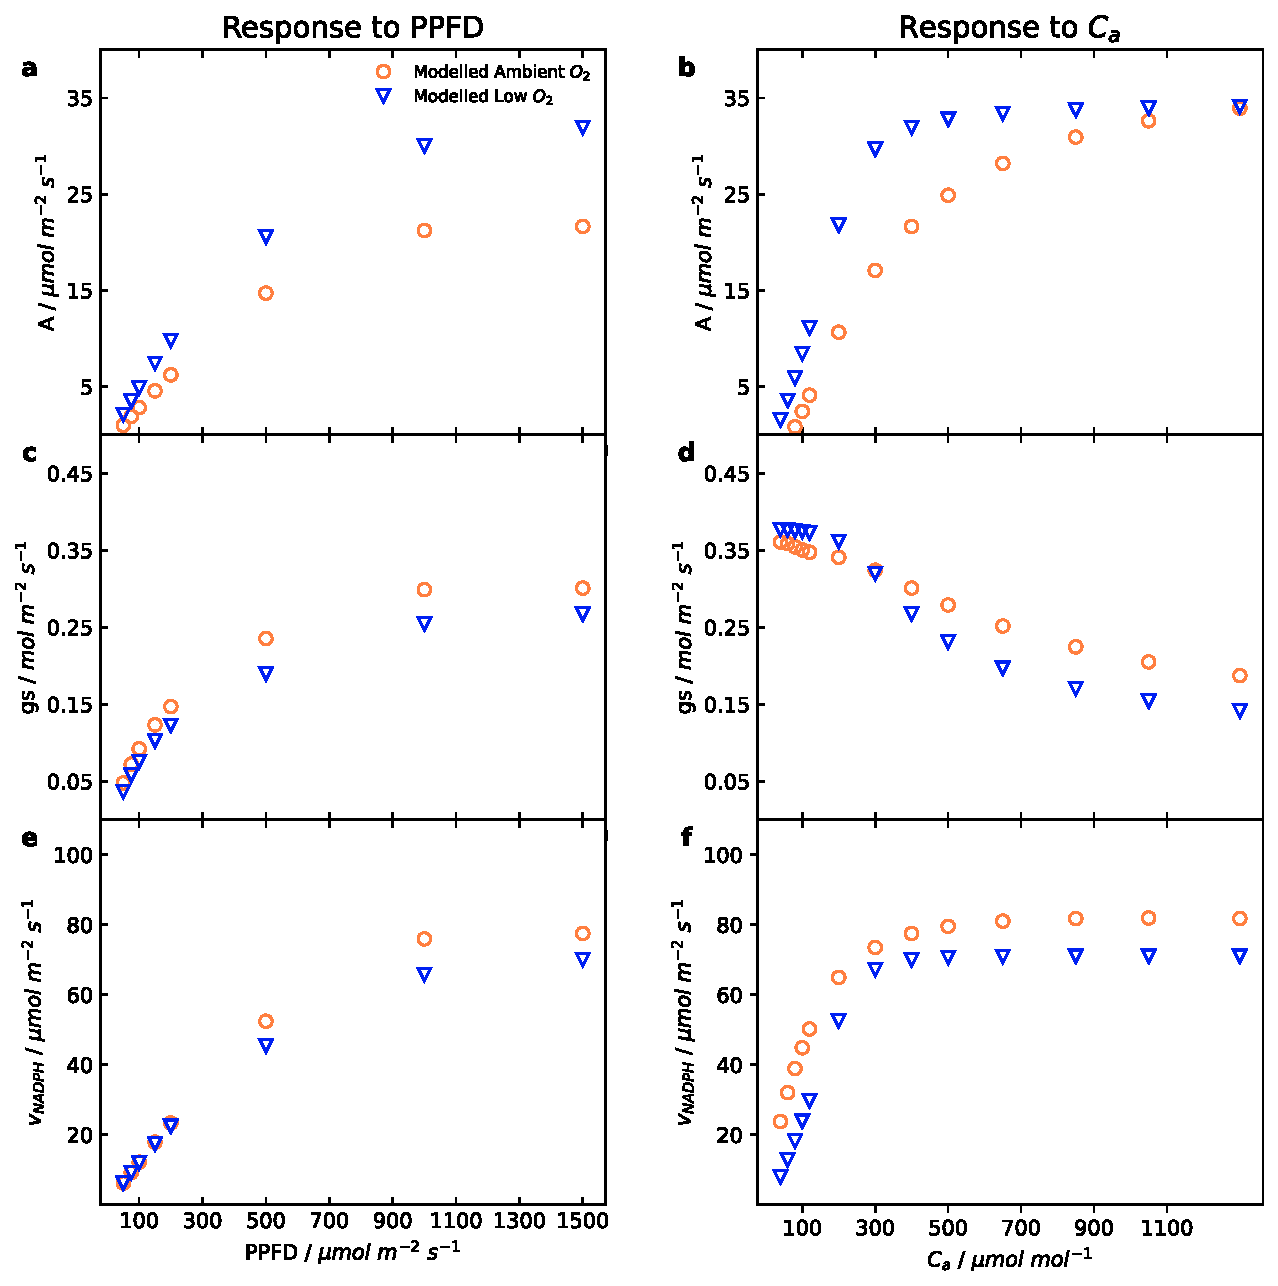
\includegraphics[width=0.7\textwidth]{Figures/Validations/bellasio2019_fig3.pdf}
    \captionvalid{Bellasio2019}{Simulated quasi-steady-state \glsentryshort{ppfd} and \glsentryshort{ca} response curves of different rates.}{A quasi-steady-state scan of \glsentryfull{ppfd} and \glsentryfull{ca} at two different \glsentryfull{o2} concentrations, \qty{210000}{\micro\barp} in orange and \qty{20000}{\micro\barp} in blue. The rates shown, from top to bottom, are \glsentryfull{A}, \glsentryfull{gs}, and \glsentryfull{vfnr}. The scan of \glsentryshort{ppfd} is done at a fixed \glsentryfull{ca} of \qty{400}{\micro\barp}, while the scan of \glsentryshort{ca} is done at a fixed \glsentryshort{ppfd} of \qty{1500}{\micro\mol\per\square\meter\per\second}. The other parameters are kept at their default values. The \glsentryshort{ppfd} values used are 50, 75, 100, 150, 200, 500, 1000, and 1500. For \glsentryshort{ca} are 400, 300, 200, 120, 100, 80, 60, 40, 400, 400, 400, 400, 500, 650, 850, 1050, and 1300. As steady-state cannot be always reached within this model, a quasi-steady-state is assumed to be at a maximum time of \qty{1800}{s}. This figure is recreated from figure 3 of the original publication of the Bellasio2019 model~\cite{bellasioGeneralisedDynamicModel2019}. The experimental data could not be plotted, as there was no access to it. In the publication it is said that a scan of \glsentryfull{ci} was done instead of \glsentryshort{ca}, however, due to many reasons, \glsentryshort{ca} is used here, even though the values of the x-axis are not identical.}
    \label{fig:bellasio2019-fig3}
\end{figure}

\begin{figure}
    \centering
    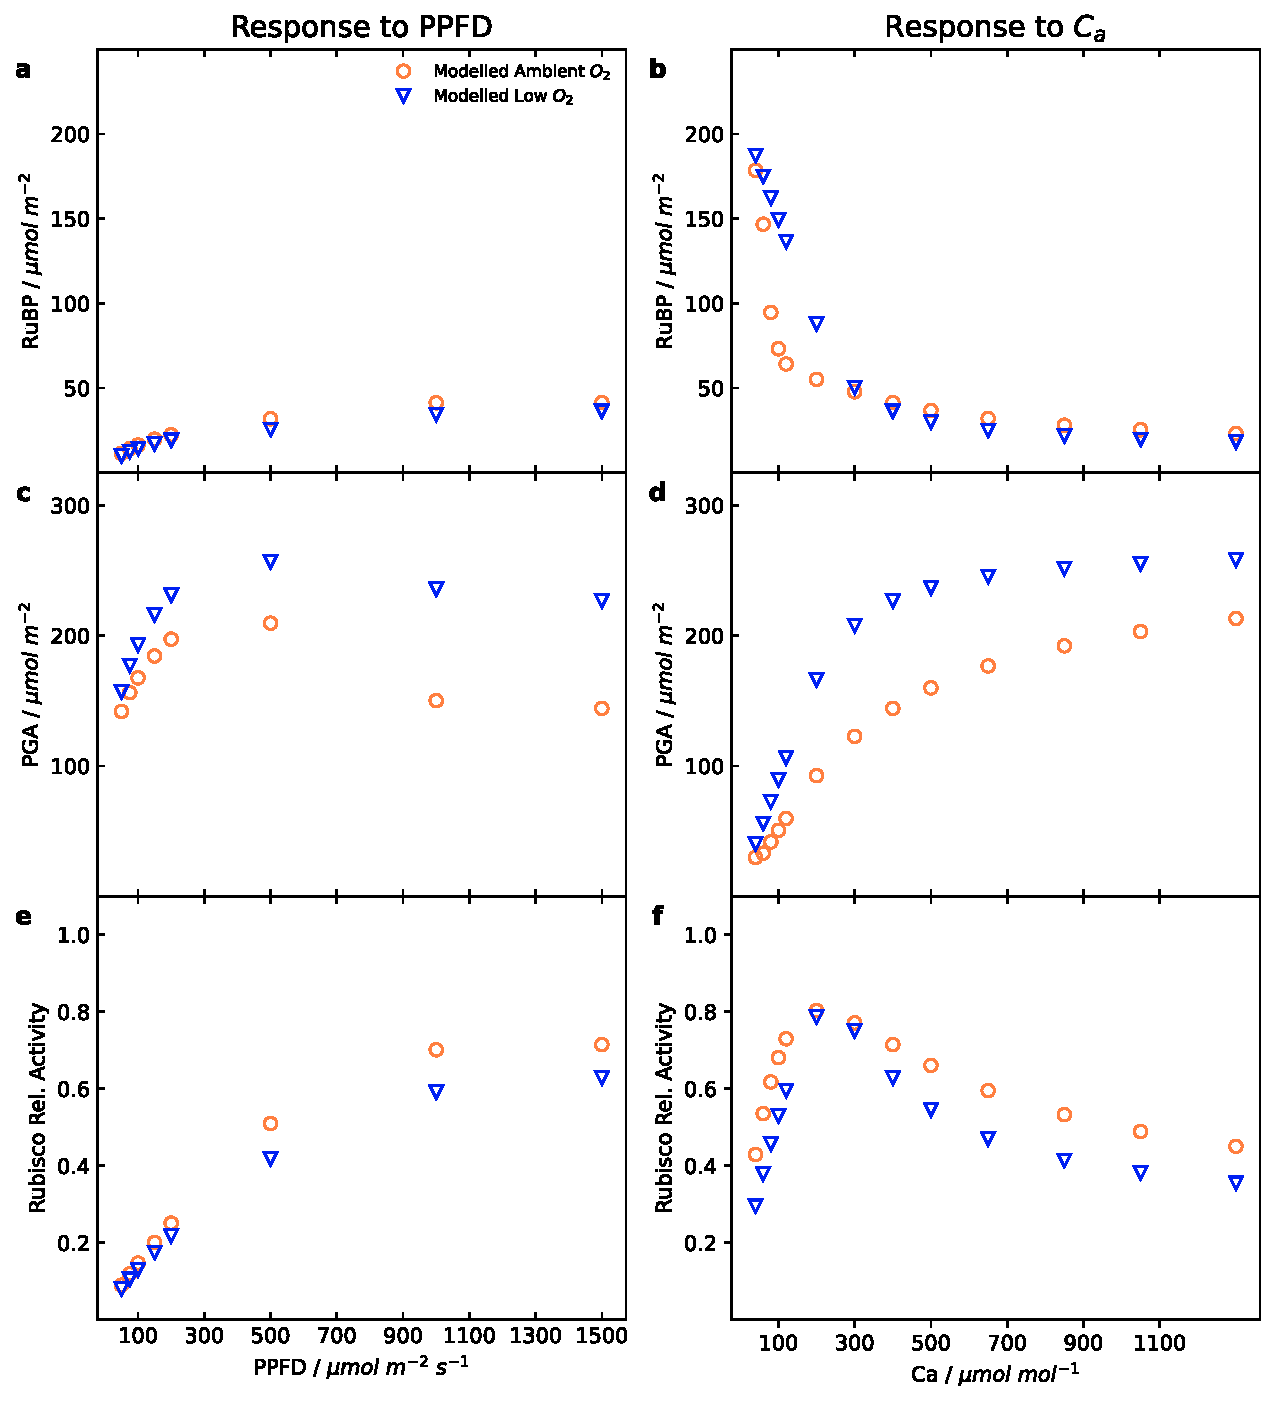
\includegraphics[width=0.7\textwidth]{Figures/Validations/bellasio2019_fig4.pdf}
    \captionvalid{Bellasio2019}{Simulated quasi-steady-state \glsentryshort{ppfd} and \glsentryshort{ca} response curves of metabolic concentrations.}{A quasi-steady-state scan of \glsentryfull{ppfd} and \glsentryfull{ca} at two different \glsentryfull{o2} concentrations, \qty{210000}{\micro\barp} in orange and \qty{20000}{\micro\barp} in blue. The metabolic concentrations shown, from top to bottom, are \glsentryfull{rubp}, \glsentryfull{pga}, and the relative \glsentryfull{rubisco} activity. The two first mentioned were multiplied by the \glsentryfull{Vm} to come to a per area unit and the last is a product of the \glsentryfull{frubp} and the \glsentryfull{Ract}. The scan of \glsentryshort{ppfd} is done at a fixed \glsentryfull{ca} of \qty{400}{\micro\barp}, while the scan of \glsentryshort{ca} is done at a fixed \glsentryshort{ppfd} of \qty{1500}{\micro\mol\per\square\meter\per\second}. The other parameters are kept at their default values. The \glsentryshort{ppfd} values used are 50, 75, 100, 150, 200, 500, 1000, and 1500. For \glsentryshort{ca} are 400, 300, 200, 120, 100, 80, 60, 40, 400, 400, 400, 400, 500, 650, 850, 1050, and 1300. As steady-state cannot be always reached within this model, a quasi-steady-state is assumed to be at a maximum time of \qty{1800}{s}. This figure is recreated from figure 4 of the original publication of the Bellasio2019 model~\cite{bellasioGeneralisedDynamicModel2019}. The experimental data could not be plotted, as there was no access to it. In the publication it is said that a scan of \glsentryfull{ci} was done instead of \glsentryshort{ca}, however, due to many reasons, \glsentryshort{ca} is used here, even though the values of the x-axis are not identical.}
    \label{fig:bellasio2019-fig4}
\end{figure}

The fifth figure has mixed results, when it comes to its recreation~\figref{fig:bellasio2019-fig5}. In all subfigures of the recreation, the first phase of the transition was kept before the zero-point of the x-axis, which is missing in the publication. This was done to make it easier to interpret if the simulation run first also had problems. The results of \gls{A}, \gls{vatp}, \gls{vfnr} at a transition of \qty{50}{\micro\mol\per\square\meter\per\second} to \qty{1500}{\micro\mol\per\square\meter\per\second} match the publication well~\figref[a]{fig:bellasio2019-fig5}, while the reverse transition shows a slightly slower acclimation to the new light intensity~\figref[b]{fig:bellasio2019-fig5}. This same issue persists with the \gls{frubp} in the high to low acclimation~\figref[d]{fig:bellasio2019-fig5}, while the \gls{frubp} in the low to high transition has the same results at the start, but ends at a lower value than the publication~\figref[c]{fig:bellasio2019-fig5}. Both the \gls{Ract} and the \gls{gs} were identically recreated~\figref[c and d]{fig:bellasio2019-fig5}. The results of \gls{pga} end at the identical value to the publication, but the transition is much faster in the low to high light and much slower in the high to low light~\figref[e and f]{fig:bellasio2019-fig5}. The \gls{Pi} results show the same slow acclimation in the low to high transition, however, the recreation recuperates from the fall to a much higher value than the publication~\figref[e]{fig:bellasio2019-fig5}. In the high to low transition, the recreation shows a small negative dip after the transition point and then rises to a stable value, while the publication, has a steady rise to a peak, which falls off a small bit to same stable value as the recreation~\figref[f]{fig:bellasio2019-fig5}. The \gls{rubp} and \gls{dhap} curves in the high to low transition both show a very similar pattern to the publication, except for the same acclimation problem explained prior with \gls{frubp}~\figref[f]{fig:bellasio2019-fig5}. On the low to high transition, however, the \gls{dhap} curve is deemed identical to the publication, while the \gls{rubp} curve shows a faster but with lower peak acclimation than the publication. On top of that, the stable value reached by the \gls{rubp} curve is also lower in the recreation\gls{frubp}~\figref[e]{fig:bellasio2019-fig5}. Lastly, both the ratios of \gls{atp} and \gls{nadph} to their respective totals show a much faster acclimation in the low to high transition, while stabilizing at a higher value than the publication~\figref[g]{fig:bellasio2019-fig5}. The same acclimation issue as with \gls{frubp} is seen in the high to low transition, while the stable value of the \gls{atp} curve is higher and of the \gls{nadph} curve is lower compared to the publication~\figref[h]{fig:bellasio2019-fig5}

\begin{figure}
    \centering
    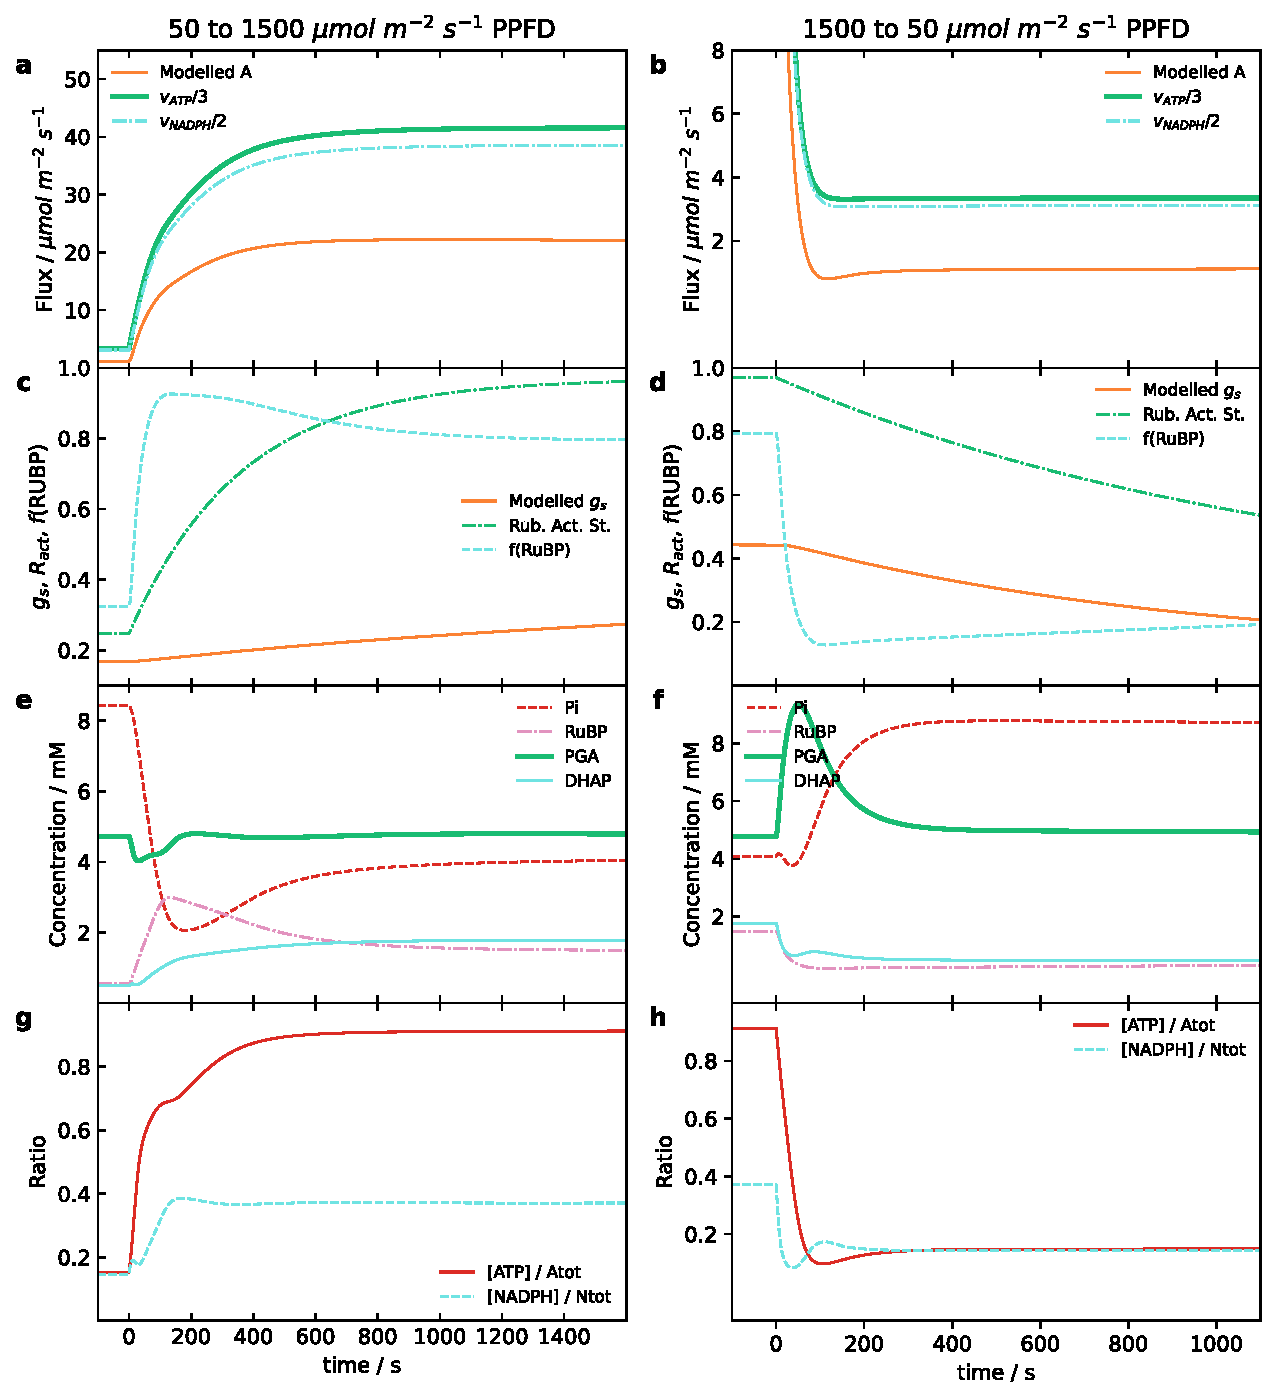
\includegraphics[width=0.7\textwidth]{Figures/Validations/bellasio2019_fig5.pdf}
    \captionvalid{Bellasio2019}{Simulated transition between different \glsentryshort{ppfd}.}{The simulations were done with an acclimation period of \qty{400}{\second} and a second period that reaches quasi-steady-state at \qty{1800}{\second}. Each period is done with a different \glsentryfull{ppfd} to show a transition. On the left, a low to high light intensity, \qty{50}{\micro\mol\per\square\meter\per\second} and \qty{1500}{\micro\mol\per\square\meter\per\second}, transition is done, while on the right the reverse is done. This switch is the zero point on the x-axis. The simulation is run using the default parameters, except \glsentryfull{ca} ($=\qty{350}{\micro\barp}$), \glsentryfull{vcmax} ($=\qty{0.18}{\milli\mol\per\meter\squared\per\second}$), \glsentryfull{tau0} ($=\qty{-0.12}{}$), \glsentryfull{Ki} ($=\qty{3600}{\second}$), and \glsentryfull{Kd} ($=\qty{1200}{\second}$). These parameters were chosen to mimic the environment of the experimental work done. The top row shows the \glsentryfull{A}, the \glsentryfull{vatp}, and \glsentryfull{vfnr}. The top-middle row shows the \glsentryfull{gs}, \glsentryfull{Ract}, and \glsentryfull{frubp}. The bottom-middle row shows the \glsentryfull{Pi}, \glsentryfull{rubp}, \glsentryfull{pga}, and \glsentryfull{dhap}. Lastly, the bottom row shows the ratio of \glsentryfull{atp} and \glsentryfull{nadph} to their respective totals. This figure is recreated from figure 5 of the original publication of the Bellasio2019 model~\cite{bellasioGeneralisedDynamicModel2019}. The experimental data could not be plotted, as there was no access to it.}
    \label{fig:bellasio2019-fig5}
\end{figure}

The sixth figure shows no similarity to the publication at all. However, many transition points, the zero-point on the axis, show a change in the slope of the continuing curves, hinting at a change in the simulation~\figref{fig:bellasio2019-fig6}. The seventh and final figure on the other hand, was successfully recreated, with both the \gls{A} and \gls{phipsii} curves showing the same pattern and values as the publication~\figref{fig:bellasio2019-fig7}. The only difference, is that the \gls{A} at the transition point of ambient to low \gls{o2} is much smoother in the recreation than it is in the publication.

\begin{figure}
    \centering
    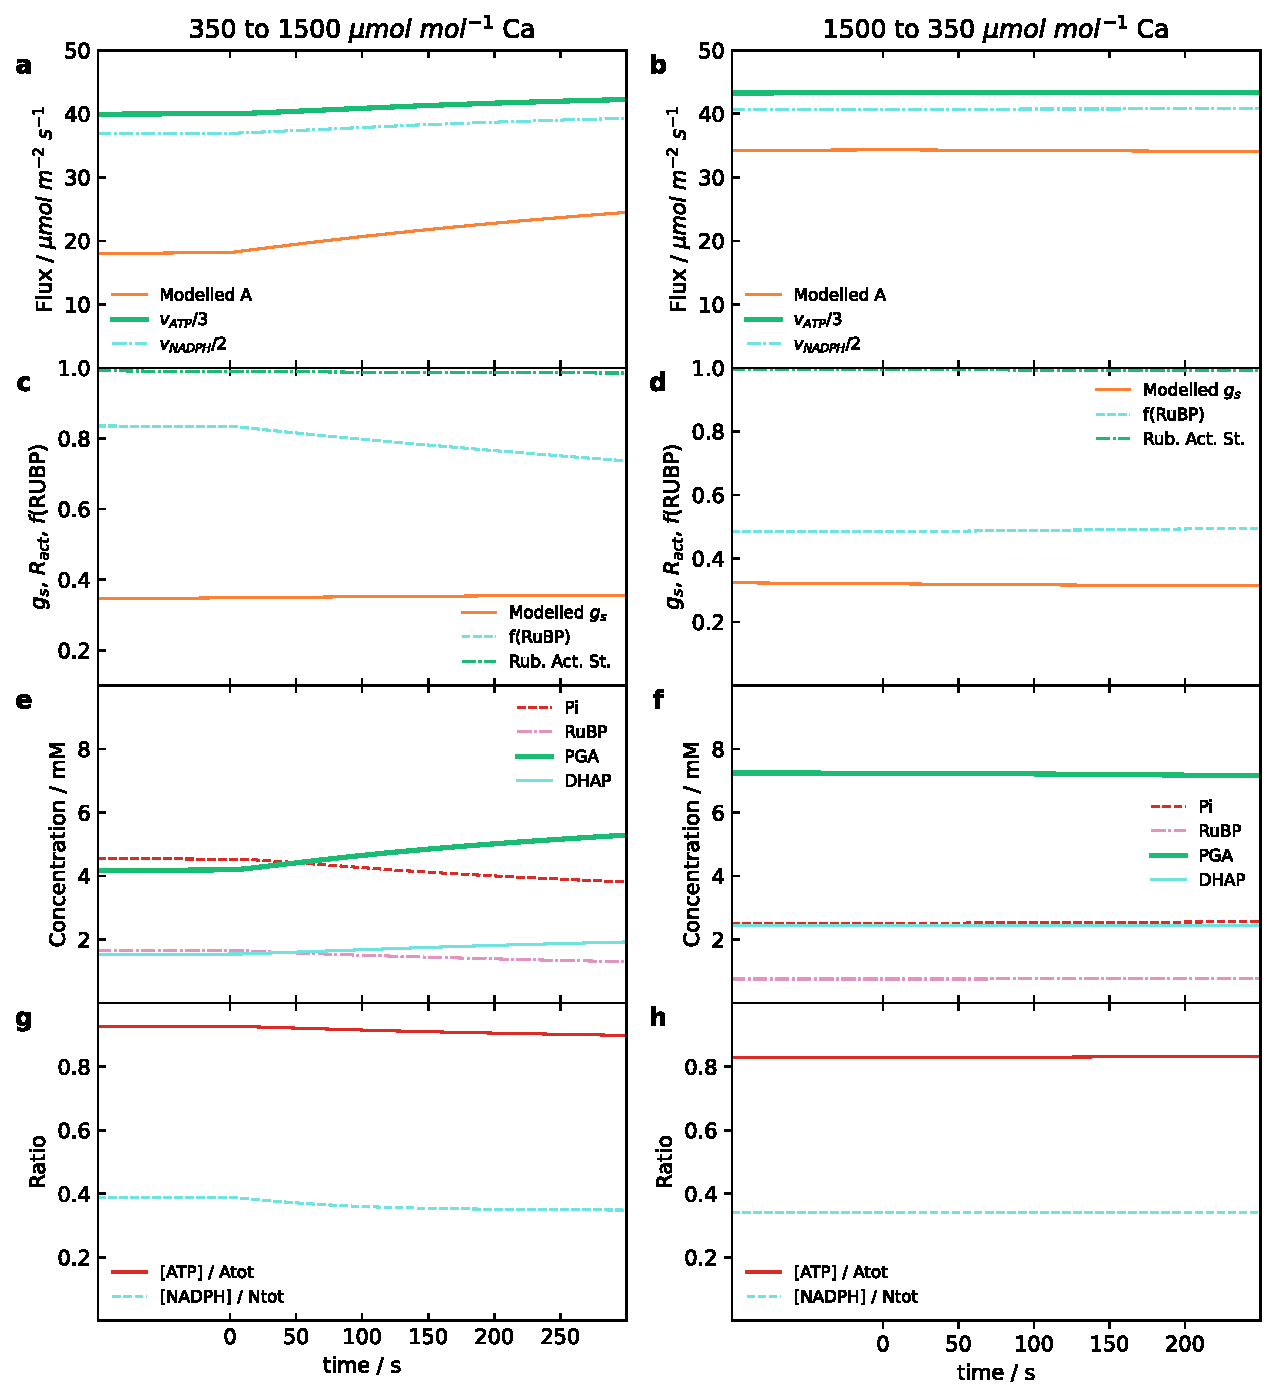
\includegraphics[width=0.7\textwidth]{Figures/Validations/bellasio2019_fig6.pdf}
    \captionvalid{Bellasio2019}{Simulated transition between different \glsentryshort{ca}.}{The simulations were done with an acclimation period of \qty{400}{\second} and a second period that reaches quasi-steady-state at \qty{500}{\second}. Each period is done with a different \glsentryfull{ca} to show a transition. On the left, an ambient to high \glsentryfull{co2} concentration, \qty{350}{\micro\barp} and \qty{1500}{\micro\barp}, transition is done, while on the right the reverse is done. This switch is the zero point on the x-axis. The simulation is run using the default parameters, except \glsentryfull{ppfd} ($=\qty{1500}{\micro\mol\per\square\meter\per\second}$), \glsentryfull{vcmax} ($=\qty{0.18}{\milli\mol\per\meter\squared\per\second}$), \glsentryfull{tau0} ($=\qty{-0.12}{}$), \glsentryfull{Ki} ($=\qty{3600}{\second}$), and \glsentryfull{Kd} ($=\qty{1200}{\second}$). These parameters were chosen to mimic the environment of the experimental work done. The top row shows the \glsentryfull{A}, the \glsentryfull{vatp}, and \glsentryfull{vfnr}. The top-middle row shows the \glsentryfull{gs}, \glsentryfull{Ract}, and \glsentryfull{frubp}. The bottom-middle row shows the \glsentryfull{Pi}, \glsentryfull{rubp}, \glsentryfull{pga}, and \glsentryfull{dhap}. Lastly, the bottom row shows the ratio of \glsentryfull{atp} and \glsentryfull{nadph} to their respective totals. This figure is recreated from figure 6 of the original publication of the Bellasio2019 model~\cite{bellasioGeneralisedDynamicModel2019}.}
    \label{fig:bellasio2019-fig6}
\end{figure}

\begin{figure}
    \centering
    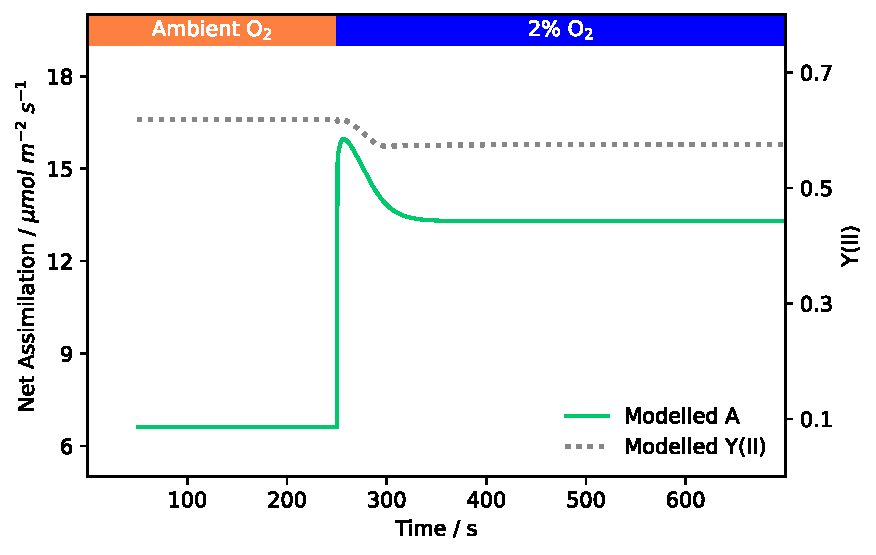
\includegraphics[width=0.7\textwidth]{Figures/Validations/bellasio2019_fig7.pdf}
    \captionvalid{Bellasio2019}{Simulated transition from ambient to low \glsentryshort{o2} concentration.}{Response of the model to a transition from ambient \glsentryfull{o2} concentration (\qty{210000}{\micro\barp}), until steady-state is reached, to low \glsentryfull{o2} concentration (\qty{20000}{\micro\barp}). The simulation is run using the default parameters, except \glsentryfull{ppfd} ($=\qty{300}{\micro\mol\per\square\meter\per\second}$) and \glsentryfull{ca} ($=\qty{200}{\micro\barp}$). Shown in the plot are \glsentryfull{A} (left y-axis) and \glsentryfull{phipsii} (right y-axis). This figure is recreated from figure 6 of the original publication of the Bellasio2019 model~\cite{bellasioGeneralisedDynamicModel2019}. The experimental data could not be plotted, as there was no access to it.}
    \label{fig:bellasio2019-fig7}
\end{figure}

\subsubsection{Fuente2024}

The recreation of the second figure of the Fuente2024 model~\cite{fuenteMathematicalModelSimulate2024} shows a good match to the publication, except for the subfigure at the top right~\figref{fig:fuente2024-fig2}. The \gls{pc_ox} curve fits the same trend as the publication, but is shifted slightly higher. The same applies to the third figure, where all but the \gls{pq_ox} and the \gls{F} curves are near to identical to the publication~\figref{fig:fuente2024-fig3}. Both inaccurate curves are shifted slightly lower in the recreation, especially noticeable in the higher light intensity range.

\begin{figure}
    \centering
    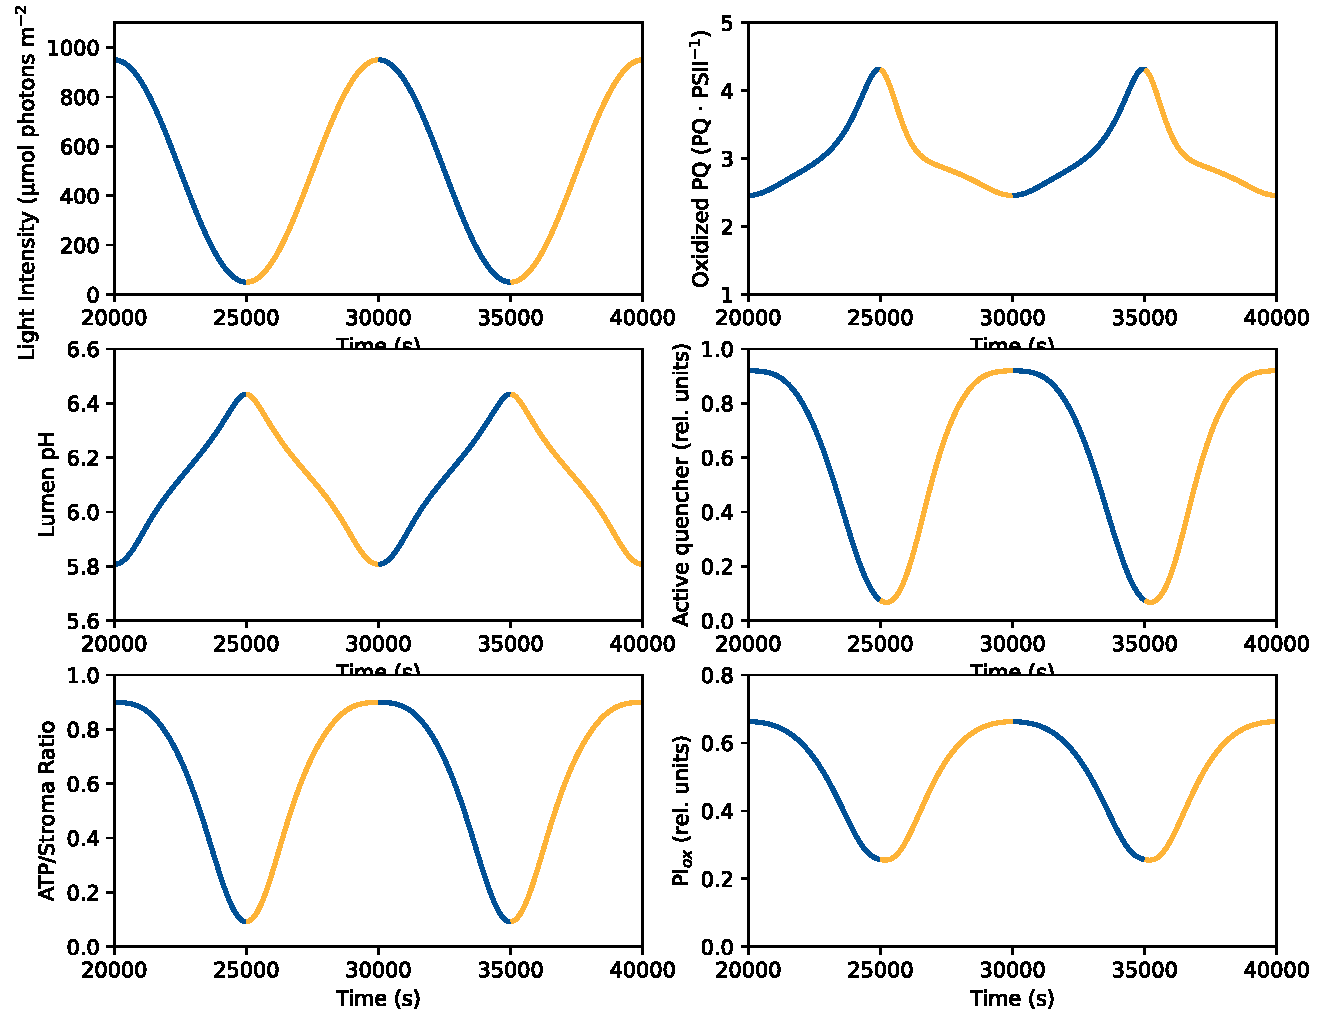
\includegraphics[width=0.7\textwidth]{Figures/Validations/fuente2024_fig2.pdf}
    \captionvalid{Fuente2024}{Results at the end of a long simulation with oscillating light.}{The light intensity used in the simulation is oscillating between \qty{50}{\micro\mol\per\square\meter\per\second} and \qty{950}{\micro\mol\per\square\meter\per\second} with a frequency of \qty[parse-numbers=false]{\frac{1}{10000}}{\per\second}, as seen in the upper left plot. The ascent of light is shown in yellow, while the descent is shown in blue. The results shown are the lumenal pH (middle left), the ratio of \glsentryfull{atp} in the stroma to the \glsentryfull{aptot} (bottom left), the \glsentryfull{pq_ox} (top right), the \glsentryfull{Qactive} (middle right), and the \glsentryfull{psiox} (bottom right). To calculate the lumenal pH, the following equation was used: $\mathrm{pH_{lu}} = -\log_{10}\left(\left[\glsentryshort{h}_\mathrm{lu}\right] \cdot 10^{-6}\right)$. The simulation is run using the default parameters and is simulated to a time of \qty{40000}{\second}, whereas only the last \qty{20000}{\second} are shown in the figure. This figure is recreated from figure 2 of the original publication of the Fuente2024 model~\cite{fuenteMathematicalModelSimulate2024}.}
    \label{fig:fuente2024-fig2}
\end{figure}

\begin{figure}
    \centering
    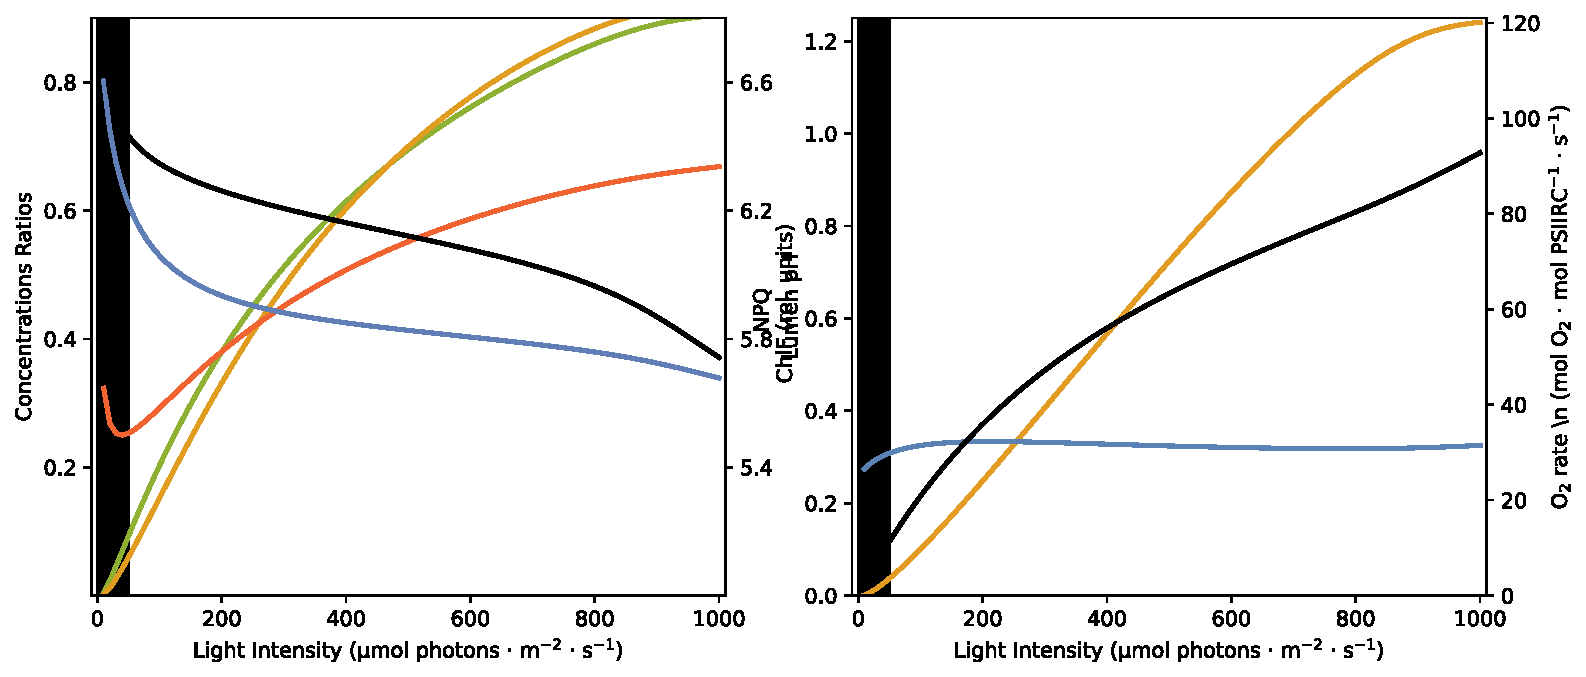
\includegraphics[width=0.7\textwidth]{Figures/Validations/fuente2024_fig3.pdf}
    \captionvalid{Fuente2024}{Steady-state scan of light intensities for several components.}{A steady-state scan of light intensities, from \qty{0}{\micro\mol\per\square\meter\per\second} to \qty{1000}{\micro\mol\per\square\meter\per\second} was done. The left plot shows the ratio of \glsentryfull{atp} in the stroma to the \glsentryfull{aptot} (green), 
    the \glsentryfull{Qactive} (yellow), the lumenal pH (black), the ratio of \glsentryfull{psiox} to the \glsentryfull{psitot} (orange), and the ratio of \glsentryfull{pq_ox} to the \glsentryfull{pqtot}. To calculate the lumenal pH, the following equation was used: $\mathrm{pH_{lu}} = -\log_{10}\left(\left[\glsentryshort{h}_\mathrm{lu}\right] \cdot 10^{-6}\right)$. The right plot shows the \gls{o2} evolution (black), the \glsentryfull{npq} (yellow), and the chlorophyll \glsentryfull{F} (blue), all directly taken from the simulation results. Note the two different y-axis on both plots to showcase different scales. The simulations are run using default parameters, while removing the oscillating light mechanism by setting the amplitude of the oscillation to zero. The light intensity is then inputted as a constant value for each simulation. This figure is recreated from figure 3 of the original publication of the Fuente2024 model~\cite{fuenteMathematicalModelSimulate2024}.}
    \label{fig:fuente2024-fig3}
\end{figure}

The fourth figure shows many similarities to the publications, yet still encompasses issues~\figref{fig:fuente2024-fig4}. The low oscillating light simulation (between \qty{50}{\micro\mol\per\square\meter\per\second} and \qty{150}{\micro\mol\per\square\meter\per\second}) shows a consistent similarity to the publication for the lumenal pH, the ratio of \gls{atp} to \gls{aptot}, and the ratio of \gls{psiox} to \gls{psitot} for all six different frequencies. The curves of the \gls{Qactive} during the low oscillating light stay true to the publication in the lower frequencies (\qty[parse-numbers=false]{\frac{1}{10000}}{\per\second}, \qty[parse-numbers=false]{\frac{1}{1000}}{\per\second}, \qty[parse-numbers=false]{\frac{1}{100}}{\per\second}, the first three rows respectively), while shifting downwards in the higher frequencies (\qty[parse-numbers=false]{}{\per\second}, \qty[parse-numbers=false]{\frac{1}{0.01}}{\per\second}, \qty[parse-numbers=false]{\frac{1}{0.001}}{\per\second}). The recreated \gls{pq_ox} in low oscillation show an upward shift in the lower frequencies, while in the frequencies of \qty[parse-numbers=false]{\frac{1}{0.01}}{\per\second} and \qty[parse-numbers=false]{\frac{1}{0.001}}{\per\second} the shift is ever so slightly down. The high oscillating light simulation (between \qty{50}{\micro\mol\per\square\meter\per\second} and \qty{950}{\micro\mol\per\square\meter\per\second}) is more consistent in its recreation, while still incorporating differences. Both the \gls{pq_ox} and the ratio of \gls{psiox} show an upward shift compared to the publication in all frequencies. In the lower frequencies (\qty[parse-numbers=false]{\frac{1}{10000}}{\per\second}, \qty[parse-numbers=false]{\frac{1}{1000}}{\per\second}, \qty[parse-numbers=false]{\frac{1}{100}}{\per\second}) the lumenal pH, the \gls{Qactive}, and the ratio of \gls{atp} all are identical to the publication. However, in the other frequencies, the latter mentioned is shifted upwards, while the other two down. It has to be noted that most mentioned shifts are minimal, except for the shifts of the \gls{Qactive} in the low frequencies of both oscillating lights and the shifts of the \gls{pq_ox} in the three highest frequencies.

\begin{figure}
    \centering
    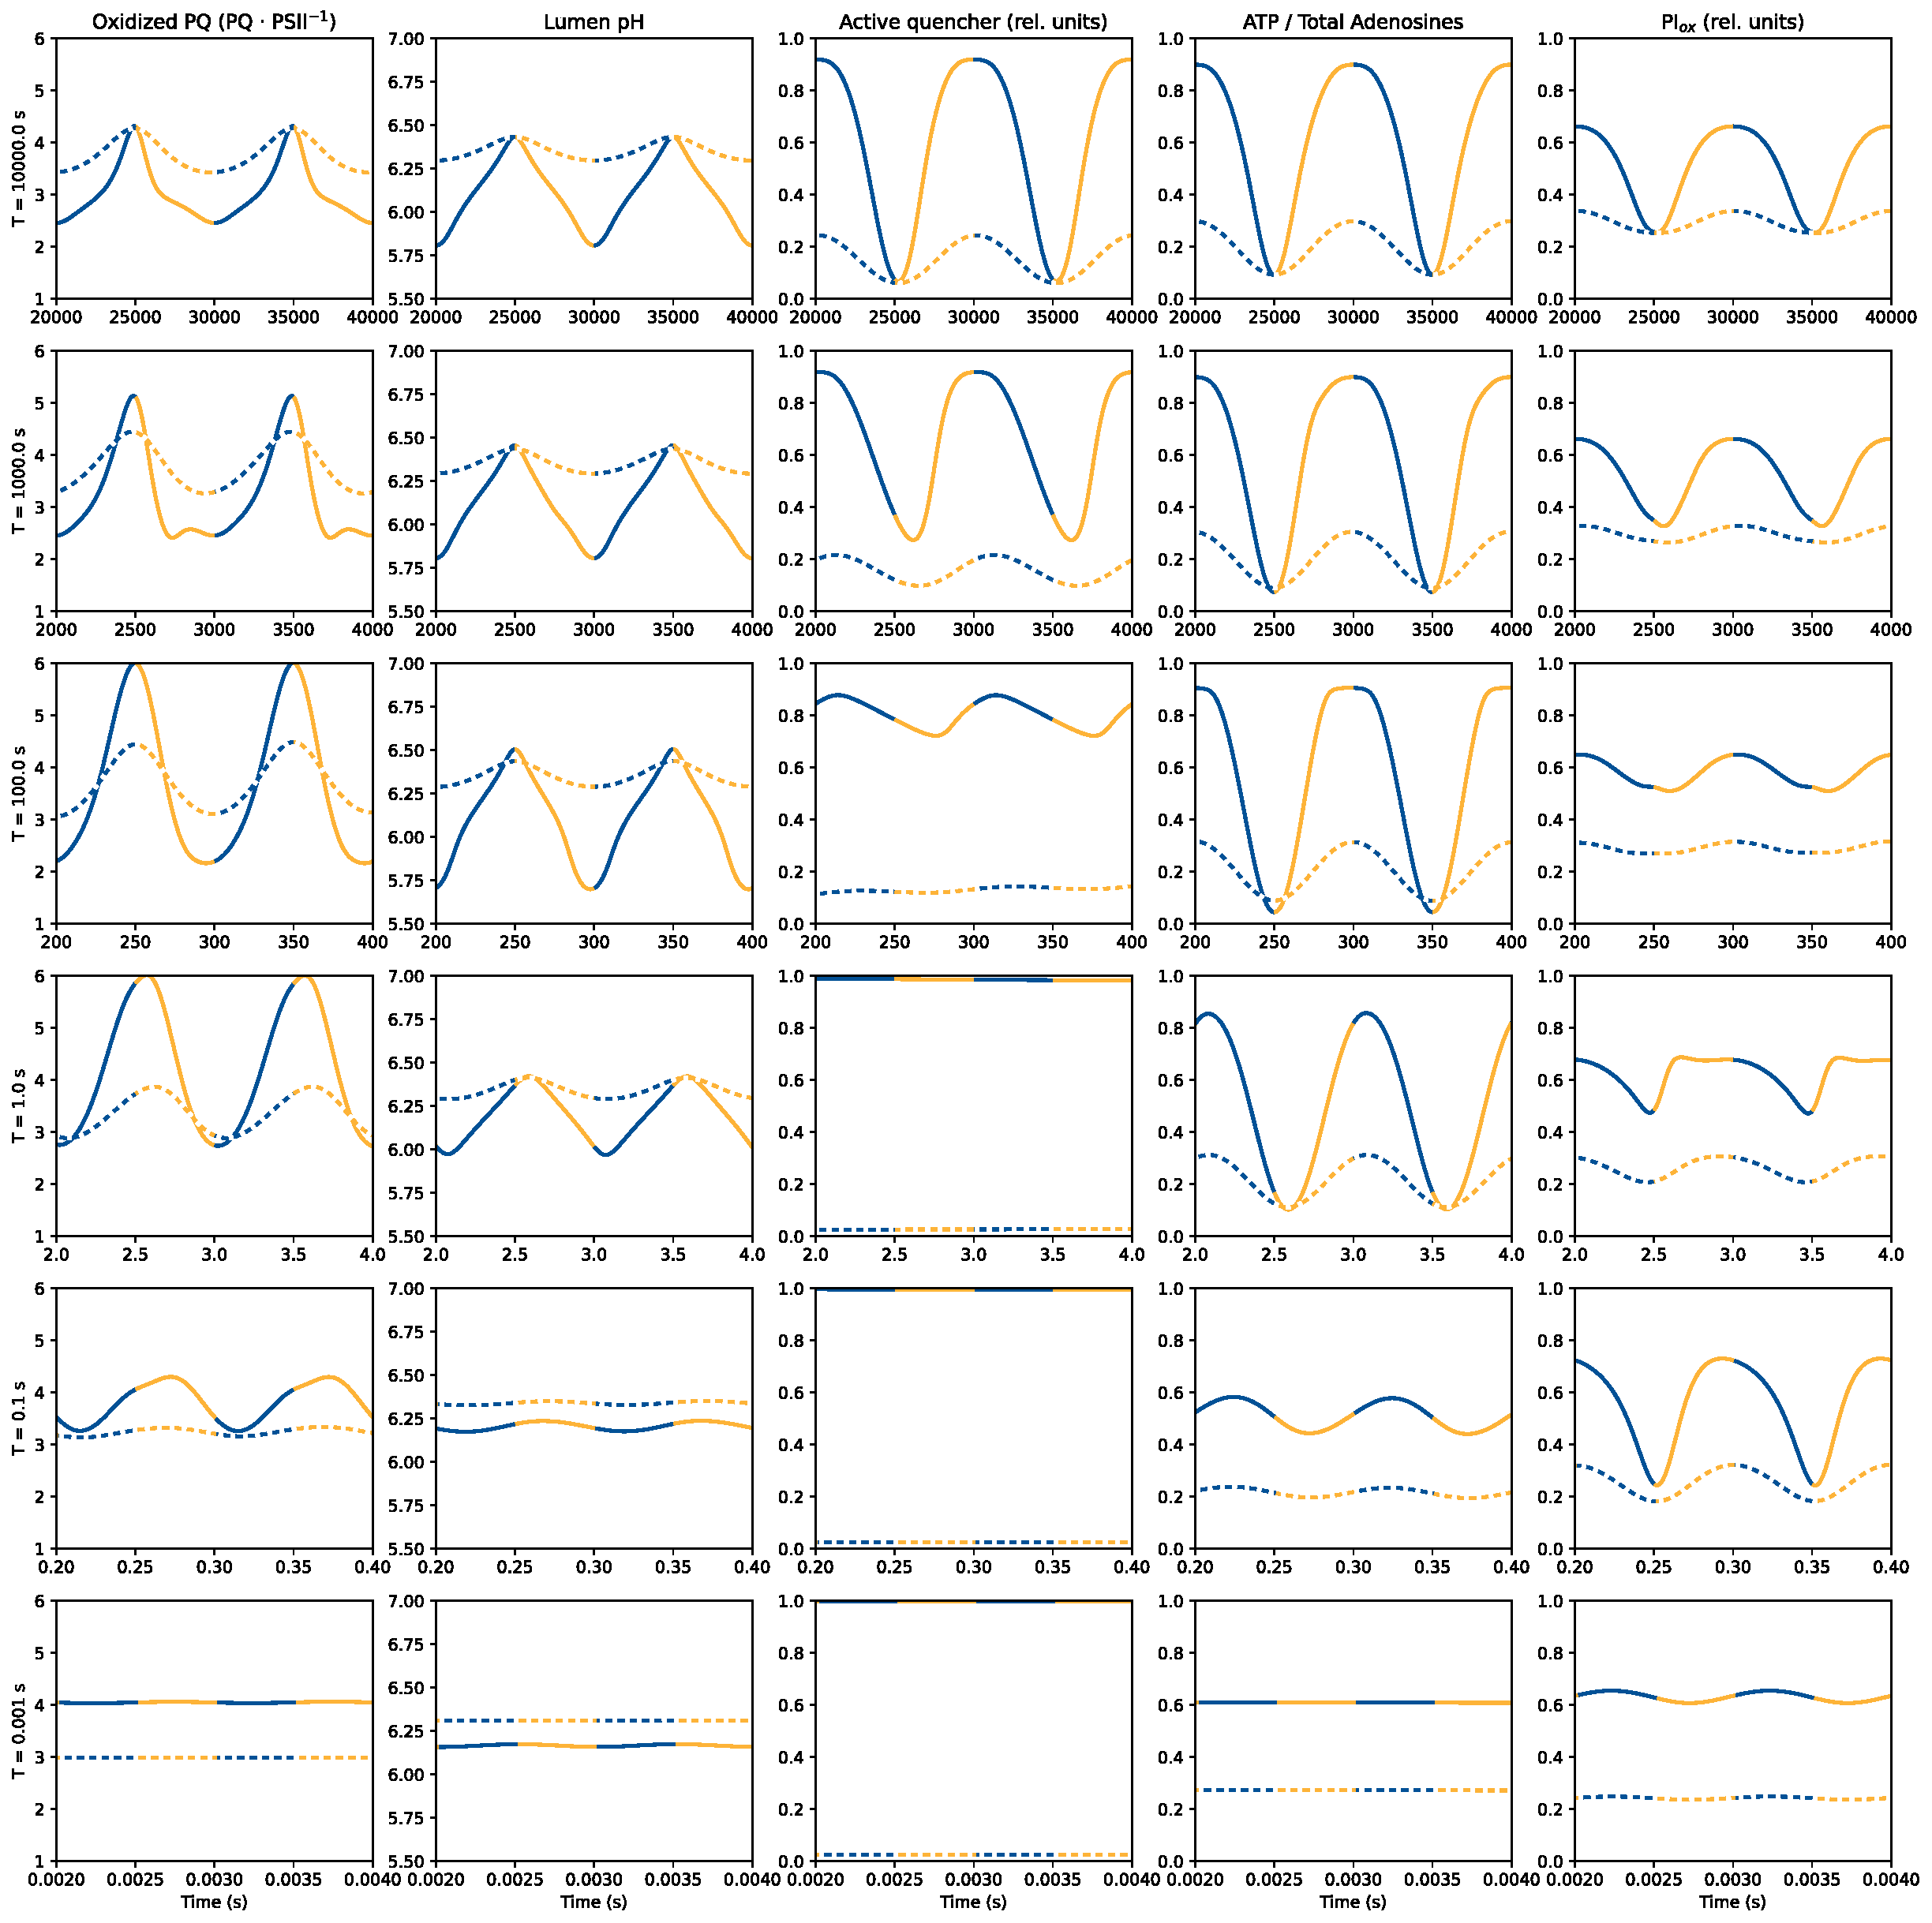
\includegraphics[width=0.7\textwidth]{Figures/Validations/fuente2024_fig4.pdf}
    \captionvalid{Fuente2024}{Results of dependent variables under differing light intensity oscillations conditions.}{Different simulations were done using different settings of the light oscillation. Each row of plots correspond to a different frequency used in the oscillation, with \qty[parse-numbers=false]{\frac{1}{10000}}{\per\second}, \qty[parse-numbers=false]{\frac{1}{1000}}{\per\second}, \qty[parse-numbers=false]{\frac{1}{100}}{\per\second}, \qty[parse-numbers=false]{\frac{1}{1}}{\per\second}, \qty[parse-numbers=false]{1}{\per\second}, and \qty[parse-numbers=false]{\frac{1}{0.001}}{\per\second}, from top to bottom. Additionally, each frequency was simulated twice with differing amplitudes of oscillation. The oscillation was either between \qty{50}{\micro\mol\per\square\meter\per\second} and \qty{950}{\micro\mol\per\square\meter\per\second} (solid) or between \qty{50}{\micro\mol\per\square\meter\per\second} and \qty{150}{\micro\mol\per\square\meter\per\second} (dashed). The ascent of light is shown in yellow, while the descent is shown in blue. The results shown are the \glsentryfull{pq_ox}, the lumenal pH, the \glsentryfull{Qactive}, the ratio of \glsentryfull{atp} in the stroma, and the \glsentryfull{psiox}, from left to right. To calculate the lumenal pH, the following equation was used: $\mathrm{pH_{lu}} = -\log_{10}\left(\left[\glsentryshort{h}_\mathrm{lu}\right] \cdot 10^{-6}\right)$. The simulations are run using the default parameters, while changing the settings of the light oscillation as described. This figure is recreated from figure 4 of the original publication of the Fuente2024 model~\cite{fuenteMathematicalModelSimulate2024}.
    }
    \label{fig:fuente2024-fig4}
\end{figure}

The fifth figure also has similar issues as the last~\figref{fig:fuente2024-fig5}. The \gls{o2} evolution rate is similar to the publication for all the frequencies at the low oscillation, while at the high oscillation it shows an upward shift in the four lower frequencies, while having a downward shift in the other frequencies. The \gls{npq} shows a good match to the publication in both oscillations for the three lower frequencies, while shifting in the higher frequencies. In the low oscillation, the \gls{npq} shifts downwards, while in the high oscillation it shifts upwards. The chlorophyll \gls{F} holds a consistent trend that is comparable to the publication in the low oscillation, and only shows a downward shift in the three highest frequencies. However, the high oscillation results not only show a shift, but also do not follow the correct curvature. In the recreation, the curves are all much more flattened than in the publication, especially in the lower frequencies.

\begin{figure}
    \centering
    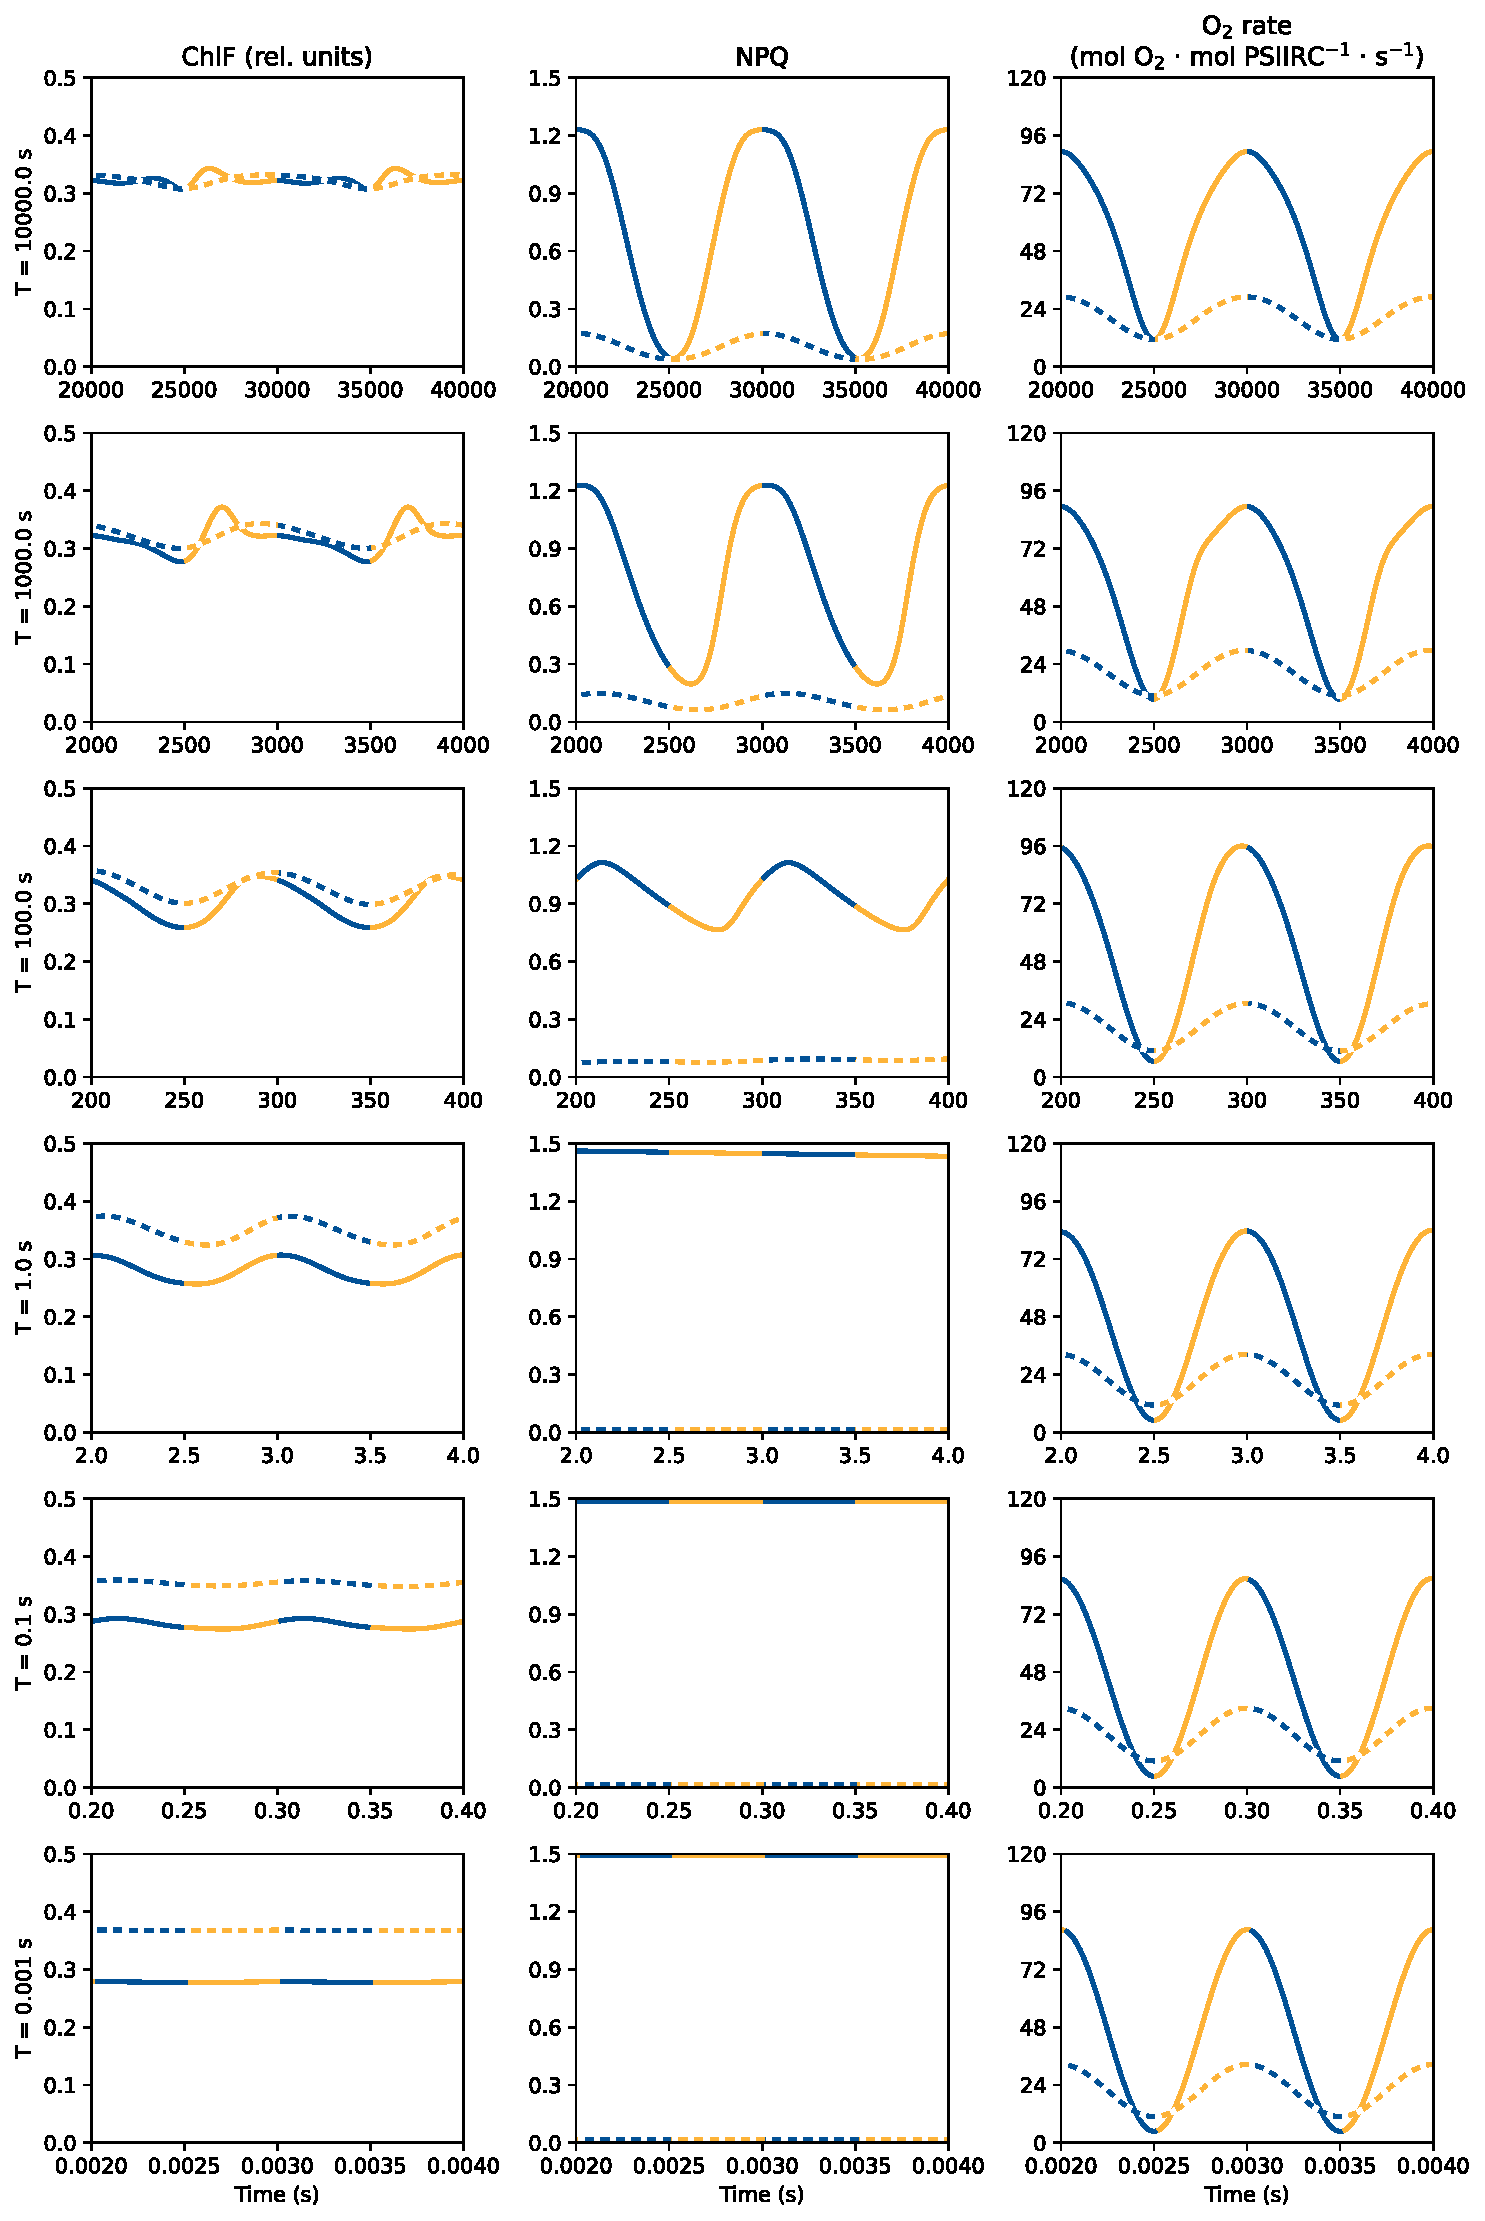
\includegraphics[width=0.7\textwidth]{Figures/Validations/fuente2024_fig5.pdf}
    \captionvalid{Fuente2024}{Results of independent variables under differing light intensity oscillations conditions.}{Different simulations were done using different settings of the light oscillation. Each row of plots correspond to a different frequency used in the oscillation, with \qty[parse-numbers=false]{\frac{1}{10000}}{\per\second}, \qty[parse-numbers=false]{\frac{1}{1000}}{\per\second}, \qty[parse-numbers=false]{\frac{1}{100}}{\per\second}, \qty[parse-numbers=false]{\frac{1}{1}}{\per\second}, \qty[parse-numbers=false]{1}{\per\second}, and \qty[parse-numbers=false]{\frac{1}{0.001}}{\per\second}, from top to bottom. Additionally, each frequency was simulated twice with differing amplitudes of oscillation. The oscillation was either between \qty{50}{\micro\mol\per\square\meter\per\second} and \qty{950}{\micro\mol\per\square\meter\per\second} (solid) or between \qty{50}{\micro\mol\per\square\meter\per\second} and \qty{150}{\micro\mol\per\square\meter\per\second} (dashed). The ascent of light is shown in yellow, while the descent is shown in blue. The results shown are the chlorophyll \glsentryfull{F}, the \glsentryfull{npq}, and the \gls{o2} evolution, from left to right. The simulations are run using the default parameters, while changing the settings of the light oscillation as described. This figure is recreated from figure 5 of the original publication of the Fuente2024 model~\cite{fuenteMathematicalModelSimulate2024}.
    }
    \label{fig:fuente2024-fig5}
\end{figure}

As the prior figures show, the implementation struggled significantly with the \gls{F}, therefore the recreation of the last three figures of the publication, all showing various aspects of this variable, was deemed not possible.

\subsubsection{Li2021}

Some subfigures of the recreation of the third figure of the Li2021 model~\cite{liImpactIonFluxes2021} show a good match to the publication~\figref{fig:li2021-fig3}. In the top row, the \gls{npq} curve of the \gls{wt} with a light intensity of \qty{500}{\micro\mol\per\square\meter\per\second} (first row, third plot) follows the same curve as the other light intensity, a stark rise at the start that forms a peak that slowly falls off to a stable value until the \qty{20}{\minute} mark, and then quickly falls to zero during the dark period. While in the publication, it slowly rises to the stable value and stays there, without first forming a peak, then also quickly drops to zero in the dark. The two last plots could not be reproduced at all, as not enough information was given to be able to recreate them using the model. The first four plots of the bottom row were able to be recreated fully, while the last three show discrepancies with the light intensity of \qty{500}{\micro\mol\per\square\meter\per\second}. As these plots show the difference between the mutant and the \gls{wt} \gls{npq}, the problem of the prior described plot persists in these plots, with the beginning of each curve being shifted upwards compared to the publication.

\begin{figure}
    \centering
    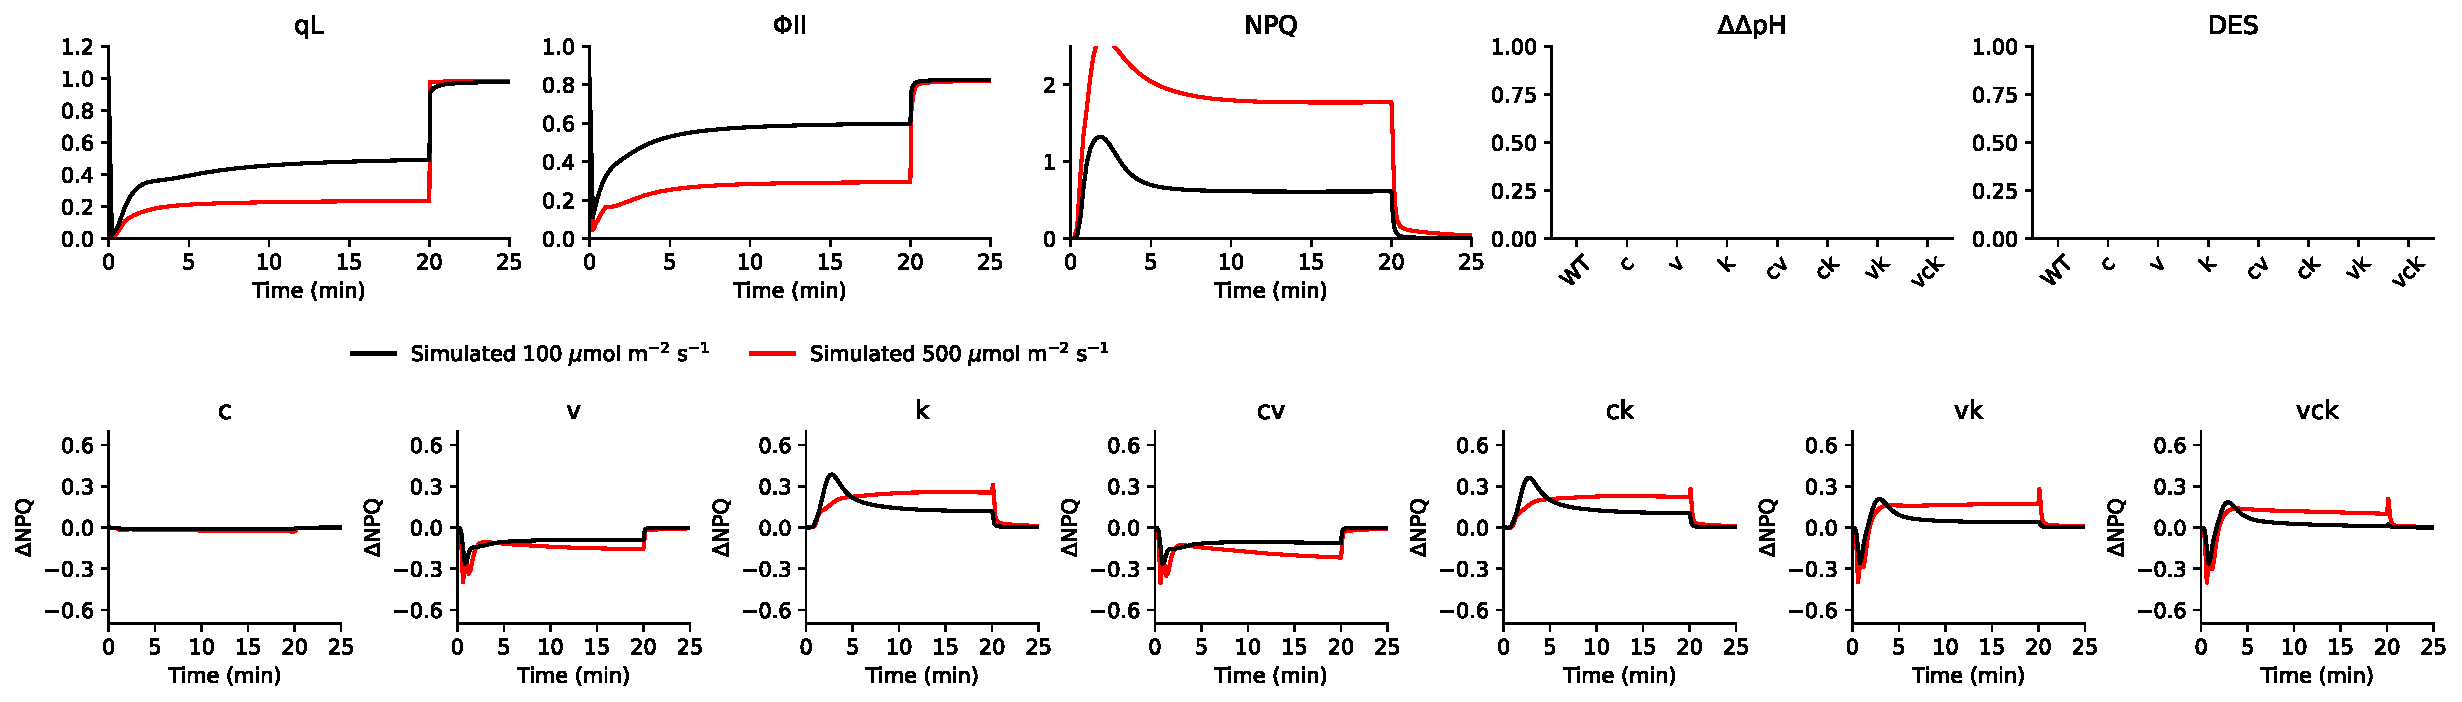
\includegraphics[width=0.7\textwidth]{Figures/Validations/li2021_fig3.pdf}
    \captionvalid{Li2021}{Simulation results of simple light protocol under differing light intensities and mutants.}{
    A simple light protocol consisting of a light period of \qty{20}{\minute}, with a light intensity of \qty{100}{\micro\mol\per\square\meter\per\second} (black) or \qty{500}{\micro\mol\per\square\meter\per\second} (red), and then a dark period of \qty{5}{\minute} was used. This protocol was simulated for several genotypes of \glsentrylong{arabidopsis}, including the \glsentryfull{wt}, and the knockout mutants of the \glsentryfull{clce} (c), \glsentryfull{vccn1} (v), \glsentryfull{kea3} (k), and every variation thereof (cv, ck, vk, vck). The results shown in the top row are the \glsentryfull{qL}, \glsentryfull{phipsii}, and the \glsentryfull{npq} of the \glsentryshort{wt} simulation, for each light intensity. Additionally, there are two empty plots, that are left to make the figure more comparable to the publication, but could not be reproduced. The bottom row shows the difference of \glsentryshort{npq} between the mutant and the \glsentryshort{wt} simulations, for both light intensities. The mutant depicted in the plot is shown in the title of each subplot. The simulations were run using the default parameters, while changing the \glsentryfull{ppfd} to match the light intensities. To create each mutant model, the corresponding rate constant of the rate being knockout was set to zero, for e.g. the rate constant of \glsentryshort{kea3} ($k_\mathrm{KEA}$). This figure is recreated from figure 4 of the original publication of the Li2021 model~\cite{liImpactIonFluxes2021}.
    }
    \label{fig:li2021-fig3}
\end{figure}

The fourth figure was recreated to a good extent, with every plot representing the \qty{100}{\micro\mol\per\square\meter\per\second} light intensity showing a good match to the publication~\figref{fig:li2021-fig4}. However, figure the \qty{500}{\micro\mol\per\square\meter\per\second} light intensity plots show a slight discrepancy, just like in the last figure. All curves follow the approximate trends, while some, like the \gls{dpH} and the \gls{pmf} curves of the \gls{wt} end at too high of a value, or the beginning of the curves show small dips and peaks, like the flux of \glsentryfull{k+lu} in the \gls{vccn1} mutant that rises and forms two peaks, one after another. These inconsistencies can be found throughout the recreated figure, however, only in the plots of the higher light intensity.

\begin{figure}
    \centering
    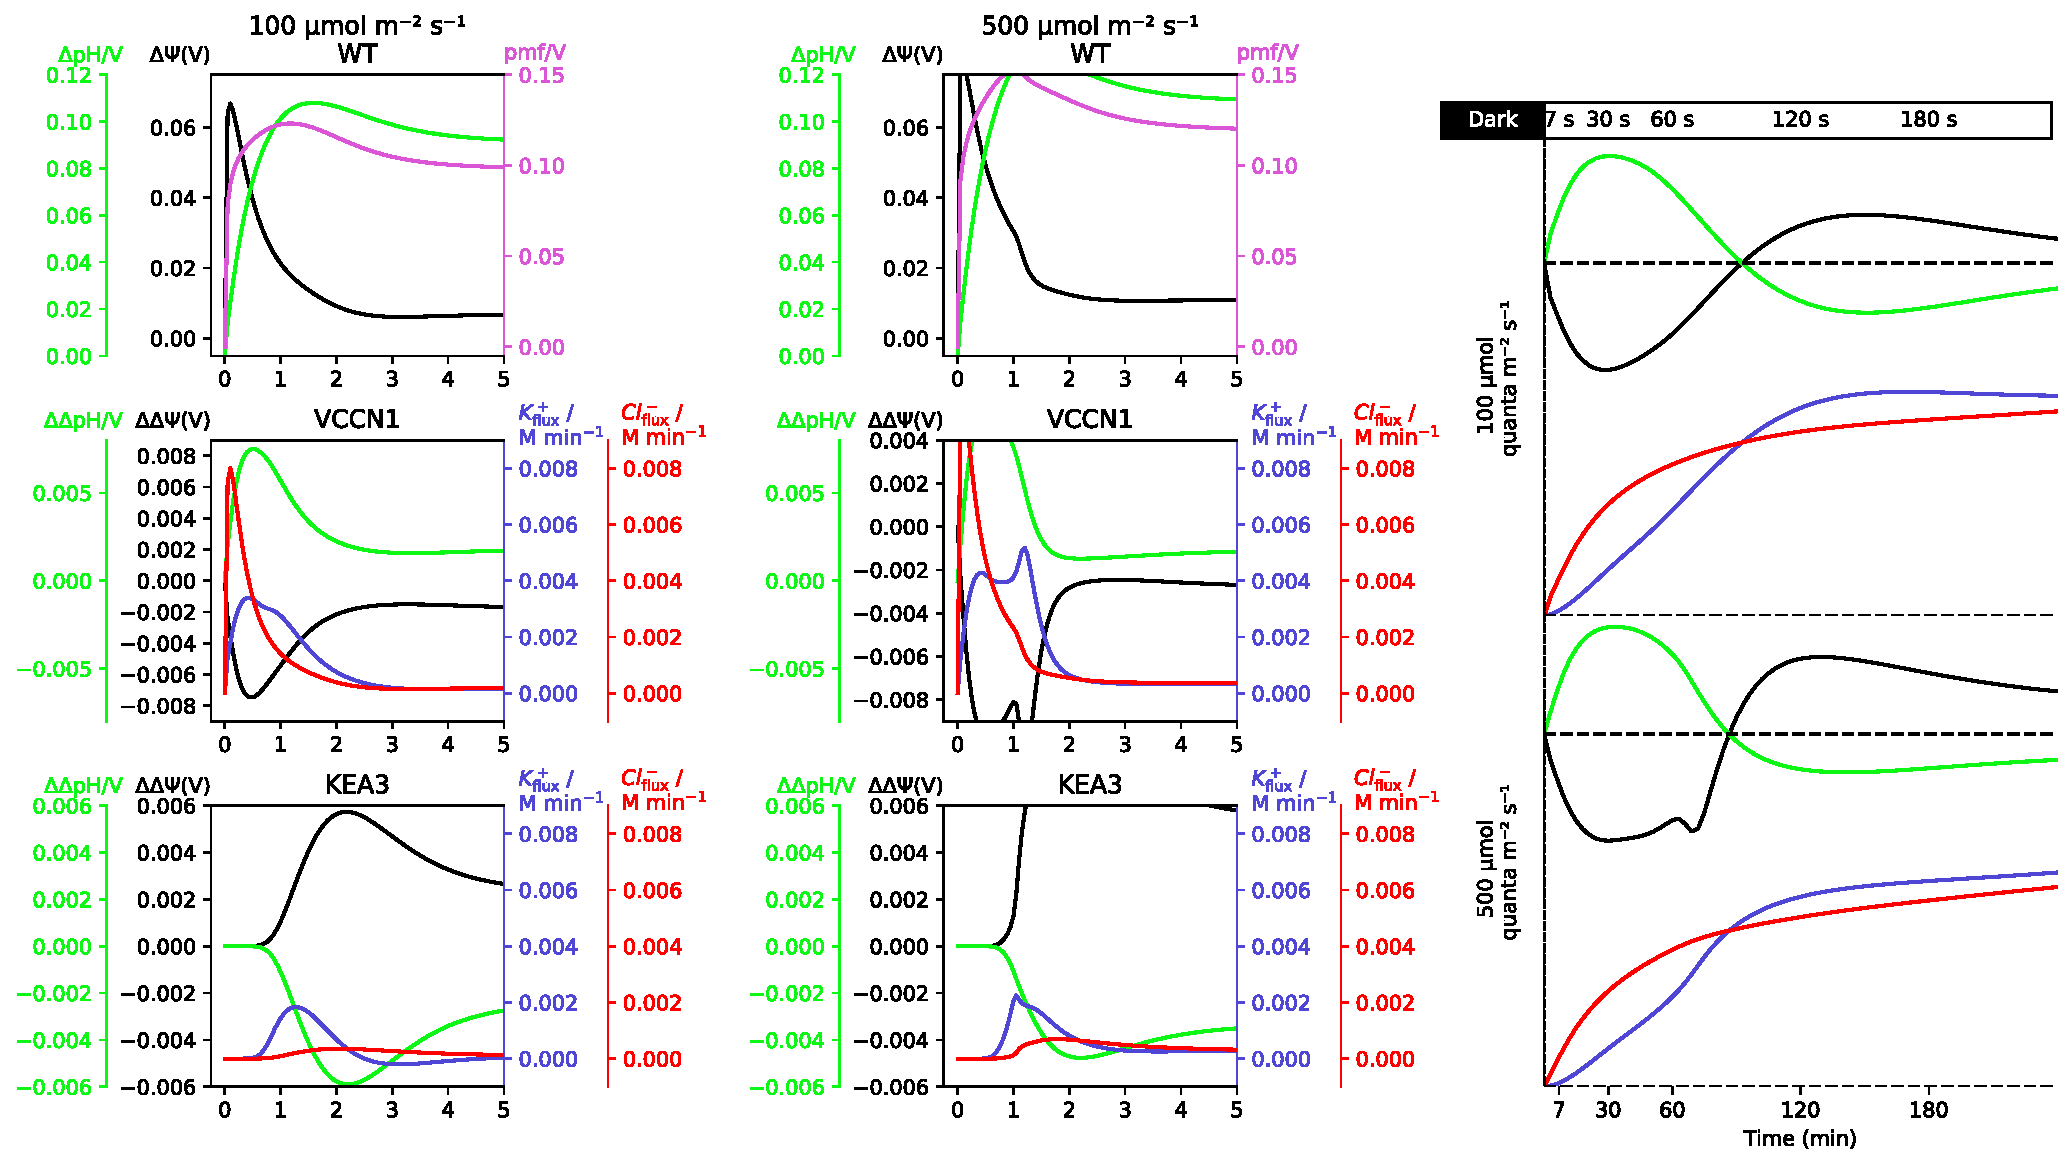
\includegraphics[width=0.7\textwidth]{Figures/Validations/li2021_fig4.pdf}
    \captionvalid{Li2021}{Simulation results of \glsentryshort{kea3} and \glsentryshort{vccn1} knockout mutants under differing light intensities.}{
    The models of the \glsentryfull{wt} (top row), \glsentryfull{vccn1} knockout mutant (middle row),  \glsentryfull{kea3} knockout mutant (bottom row), and the combination of both with the additional \glsentryfull{clce} knockout (right column) were simulated under a light intensity of \qty{100}{\micro\mol\per\square\meter\per\second} (left column, and top row of right column), \qty{500}{\micro\mol\per\square\meter\per\second} (middle column and bottom row of right column). The results shown in the top row of the two left columns are the \glsentryfull{pmf} (pink), the \glsentryfull{dpH} (green), and the \glsentryfull{dpsi} (black), all in Volts, for the \glsentryshort{wt}. In the two last rows of the left columns all curves are differences between the \glsentryshort{wt} and corresponding mutant. These results are the \glsentryfull{dpH} (green) and the \glsentryfull{dpsi} (black) and the fluxes of the \glsentryfull{k+lu} (blue) and \glsentryfull{cl-lu} (red). The fluxes are taken from the model, by getting the right-hand side of each time point of the corresponding \glsentryfull{ode} and by multiplying by 60, to convert from per second to per minute. The same results are plotted on the right column. The simulations were run using the default parameters, while changing the \glsentryfull{ppfd} to match the light intensities. To create each mutant model, the corresponding rate constant of the rate being knockout was set to zero, for e.g. the rate constant of \glsentryshort{kea3} ($k_\mathrm{KEA}$). This figure is recreated from figure 4 of the original publication of the Li2021 model~\cite{liImpactIonFluxes2021}.
    }
    \label{fig:li2021-fig4}
\end{figure}

The recreation of the fifth figure has also some mixed results~\figref{fig:li2021-fig5}. The top row shows a good representation of the first plot, but the second plot has the same problem as the prior plots. The \gls{npq} difference of the \qty{500}{\micro\mol\per\square\meter\per\second} light intensity curve has a too strong rise at the beginning, while getting to the same stable value as the publication. These issues can also be seen in the last plot of the first row, as this plot shows a \qty{2}{\minute} scan of the differences of \gls{npq} at different light intensities. Therefore, all curves in this plot are shifted upwards in comparison to the publication. The first two plots of the middle row show a very good recreation of the publication, while the curve for \gls{vccn1} in the last plot ends at a slightly too high value, compared to the publication. The bottom row starts out with a good match in the first column, but the middle column shows some small mismatches. In both initial plots, the points of the multiplier factor of 10 and 100 are shifted away from the zero point for the \gls{kea3} mutant, while they shift to the zero point for the \gls{vccn1} mutant, compared to the publication. However, the steady-state plots both are a good match to the publication, which cannot be said to the last plot of the bottom row. All the points of the higher multiplier factors are a good match, however, the points of both light intensities of the lower factors are shifted both upwards, where the \qty{500}{\micro\mol\per\square\meter\per\second} light intensity points are shifted much more than the \qty{100}{\micro\mol\per\square\meter\per\second} light intensity points.
\begin{figure}
    \centering
    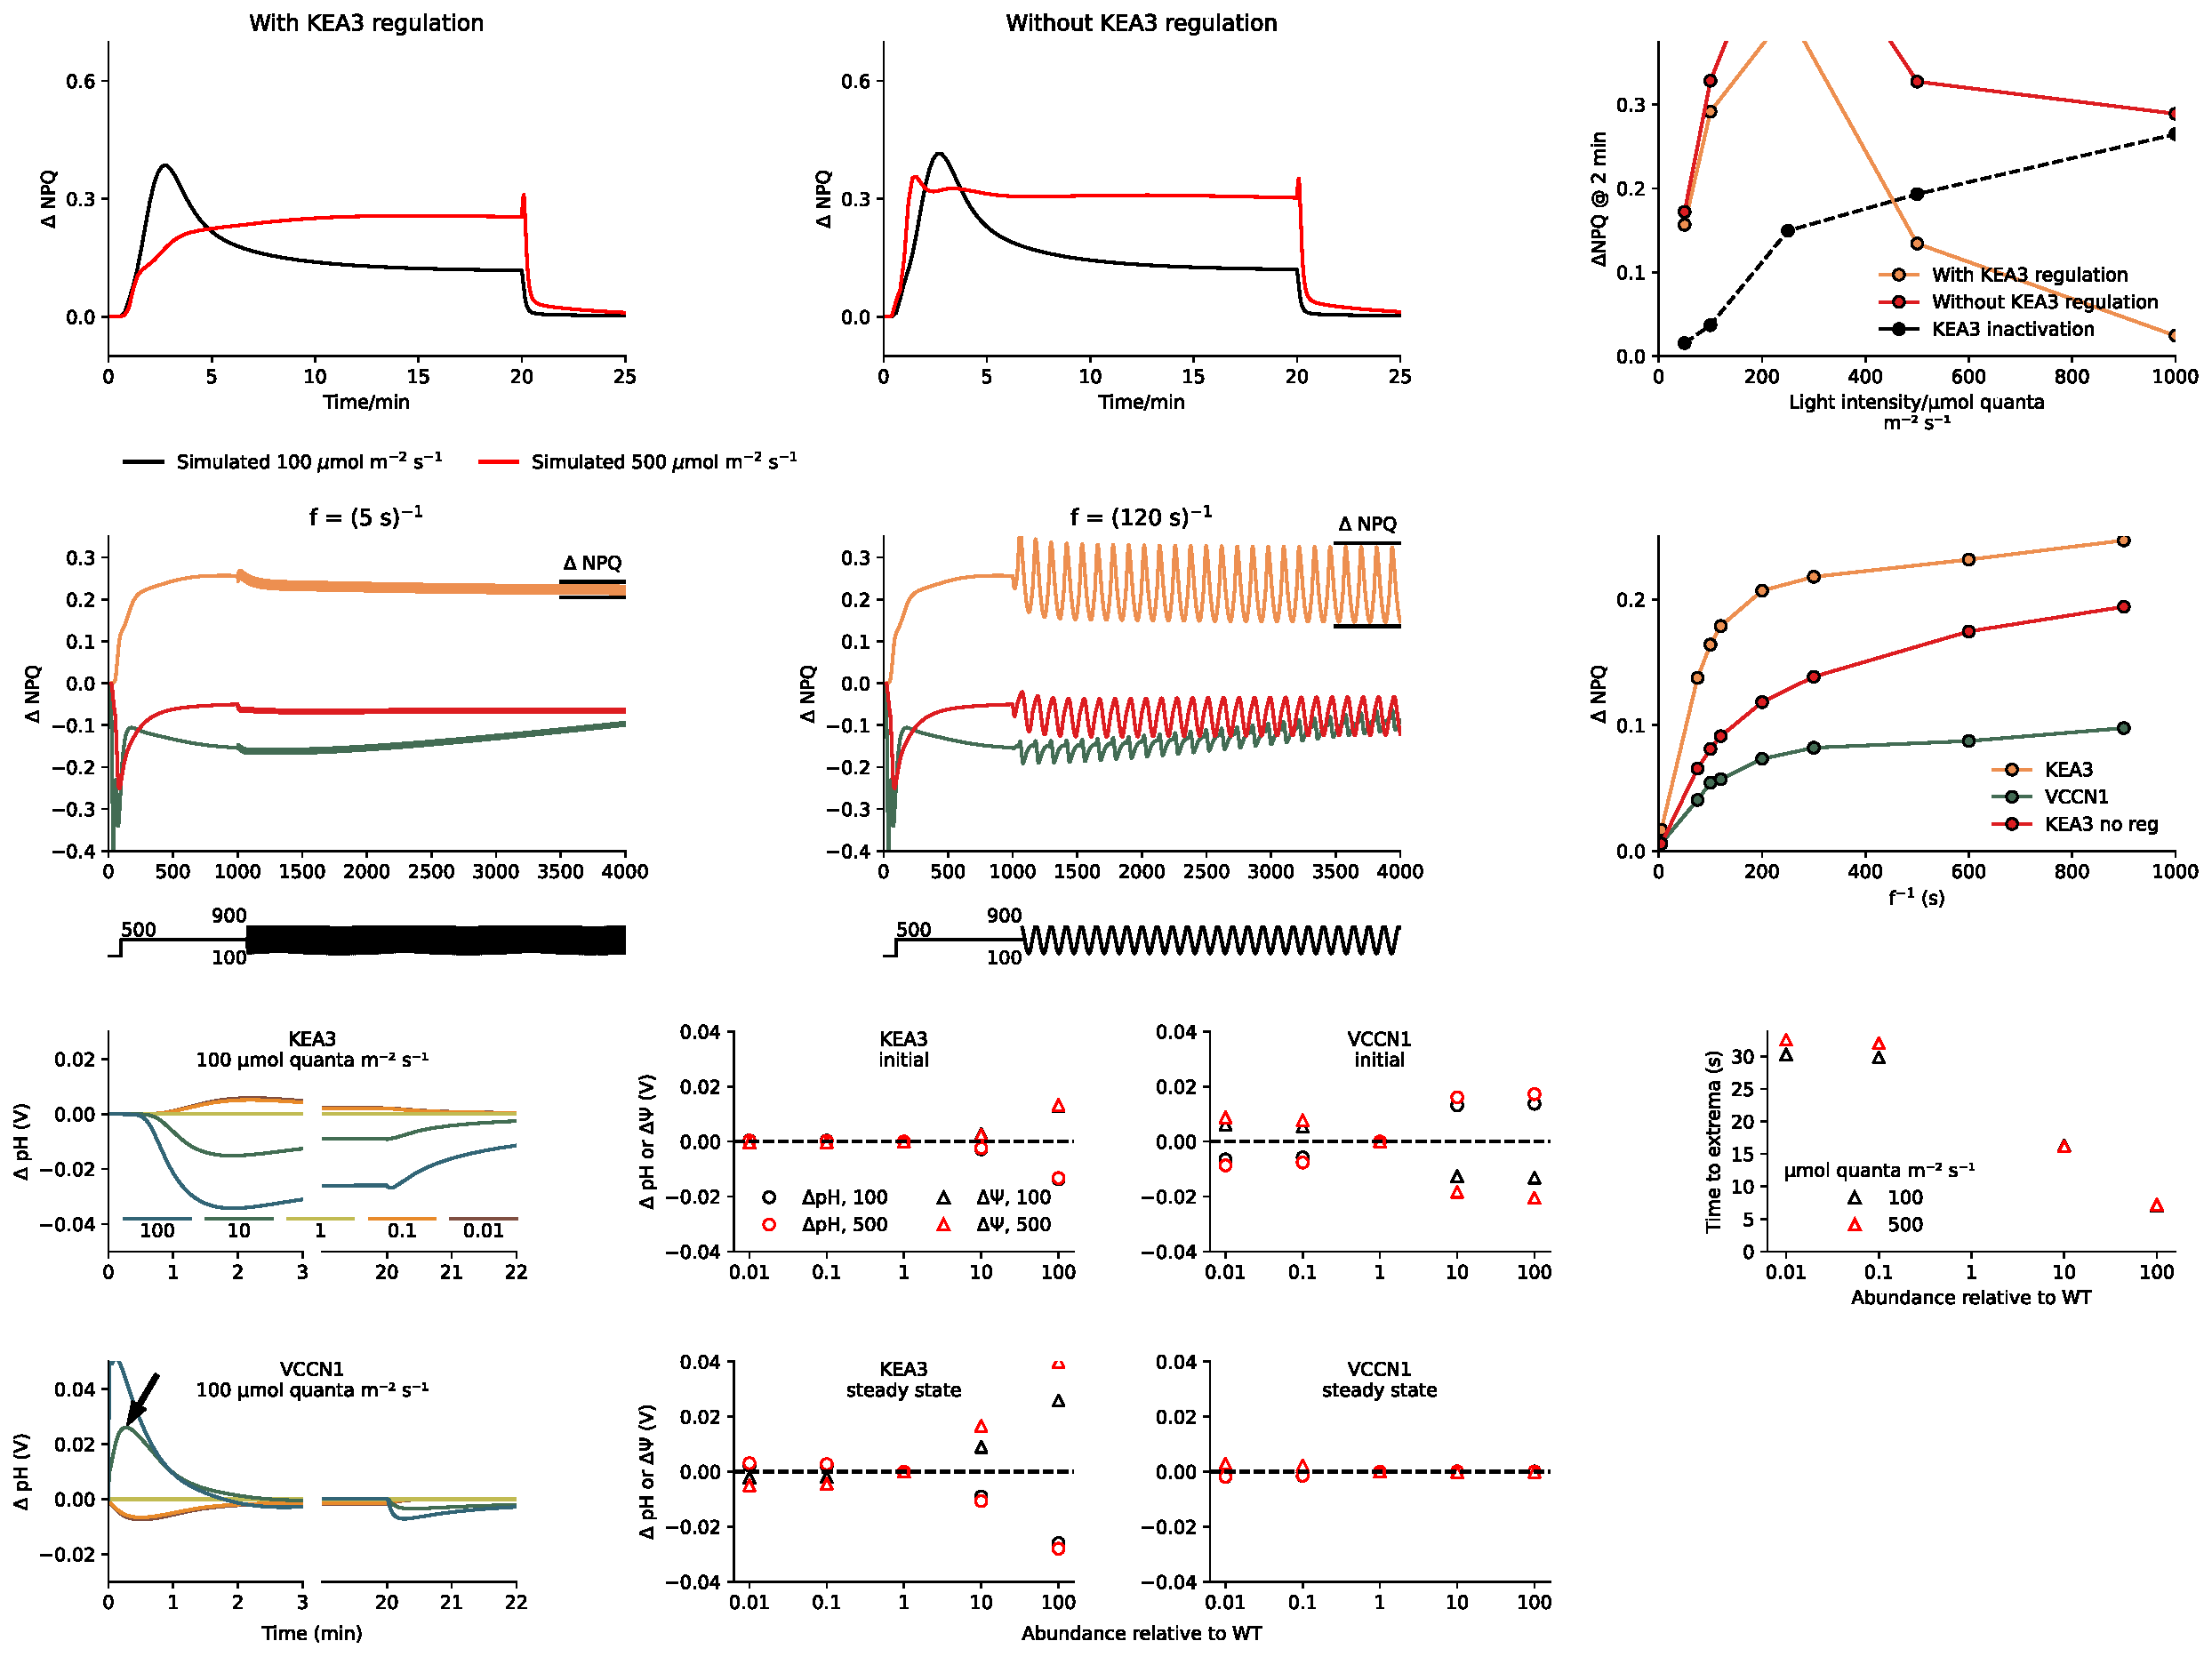
\includegraphics[width=0.7\textwidth]{Figures/Validations/li2021_fig5.pdf}
    \captionvalid{Li2021}{Simulation results of \glsentryshort{kea3} regulation, oscillating light, and different abundances of \glsentryshort{kea3} and \gls{vccn1}.}{
    Three different types of simulation was performed here. The top row shows results of simulations that show the effect of \glsentryfull{kea3} regulation. The first two plots show the results of a simulation following a simple light protocol, with a light period of \qty{20}{\minute} and a dark period of \qty{5}{\minute}. Each plot consists of two simulations, each showing a simulation at either a light intensity of \qty{100}{\micro\mol\per\square\meter\per\second} (black) or \qty{500}{\micro\mol\per\square\meter\per\second} (red). The left plot describes difference of the \glsentryshort{kea3} knockout mutant to the \glsentryshort{wt} simulation, while the right plot describes the difference of a simulation without the \glsentryfull{kea3} regulation mechanism to the \glsentryshort{wt} simulation. To remove the regulation of \glsentryshort{kea3}, the \glsentryfull{qlact} was set to a constant value of one. These plots show the \glsentryfull{npq} over the time series, which is also shown on the right plot, however, as a scan of light intensities at the \qty{2}{\minute} mark. Additionally, a difference curve is also drawn in the plot (black and dashed). The middle row shows the reaction of the model to oscillating light. To simulate this new form of light, a simple sinus curve was used, with the following equation: $\mathrm{PPFD} = \mathrm{PPFD_{base}} + \mathrm{PPFD_{amp}} \cdot \sin\left(2 \pi \cdot \mathrm{f} \cdot t\right)$. In this equation, the $\mathrm{PPFD_{base}}$ shows the value where the oscillation should happen, the $\mathrm{PPFD_{amp}}$ shows the amplitude of the oscillation, and the $\mathrm{f}$ shows the frequency of the oscillation. The two first plots show the difference of \glsentryshort{npq} to the \glsentryshort{wt} of the \glsentryshort{kea3}, \glsentryfull{vccn1}, and without \glsentryshort{kea3} regulation mutants, at two different frequencies. The left at a frequency of \qty[parse-numbers=false]{\frac{1}{5}}{\per\second}, and the right at a frequency of \qty[parse-numbers=false]{\frac{1}{120}}{\per\second}. The simulations were first run to \qty{1000}{\second}
    at a light intensity of \qty{500}{\micro\mol\per\square\meter\per\second} without any oscillation, and then until \qty{4000}{\second} with an oscillation  between \qty{100}{\micro\mol\per\square\meter\per\second} and \qty{900}{\micro\mol\per\square\meter\per\second}. The last plot shows the difference between the extrema of the last wave at varying frequencies of all three mutants. The last row shows the effect of different abundances of \glsentryshort{kea3} and \glsentryshort{vccn1} on the \glsentryfull{dpH} and \glsentryfull{dpsi}. The abundance of either \glsentryshort{kea3} or \glsentryshort{vccn1} was changed by a factor of 100, 10, 1, 0.1, and 0.01, by multiplying the factor to the respective rate constant of the transporter. The simulations run follow the same light protocol as the first row, show the difference of \glsentryshort{dpH} to the normal abundance (1) as a time series for \qty{100}{\micro\mol\per\square\meter\per\second}. The four plots in the middle show the initial and steady-state values of \glsentryshort{dpH} (circles) and \glsentryshort{dpsi} (triangles) at \qty{100}{\micro\mol\per\square\meter\per\second} (black) and \qty{500}{\micro\mol\per\square\meter\per\second} (red), for each abundance, also as a difference to the normal abundance. The initial values were taken as a difference of the value at \qty{50}{\second} to the start of the respective simulation, while the steady-state values were taken at \qty{20}{\minute}. The last plot on the right shows the time it took to reach the extrema of the \glsentryshort{vccn1} abundance time series. An example is marked as an arrow in the bottom left plot. The time point of the extrema of both light intensities is then plotted. All simulations named here were run using the default parameters, unless stated otherwise. To create each mutant model, the corresponding rate constant of the rate being knockout was set to zero, for e.g. the rate constant of \glsentryshort{kea3} ($k_\mathrm{KEA}$). This figure is recreated from figure 5 of the original publication of the Li2021 model~\cite{liImpactIonFluxes2021}.
    }
    \label{fig:li2021-fig5}
\end{figure}

\subsubsection{Matuszynska2016}

In the recreation of the fourth figure of the Matuszynska2016 model~\cite{matuszynskaMathematicalModelNonphotochemical2016}, all three plots show a very good match to the publication~\figref{fig:matuszynska2016-fig4}. As access to the experimental data was possible was given, the experimental values were also plotted. The only thing to note, is that these data points had to be shifted on the x-axis to fit the actual peaks of the simulation. It is assumed that, that was also done for the publication, which is why it was done here.

\begin{figure}
    \centering
    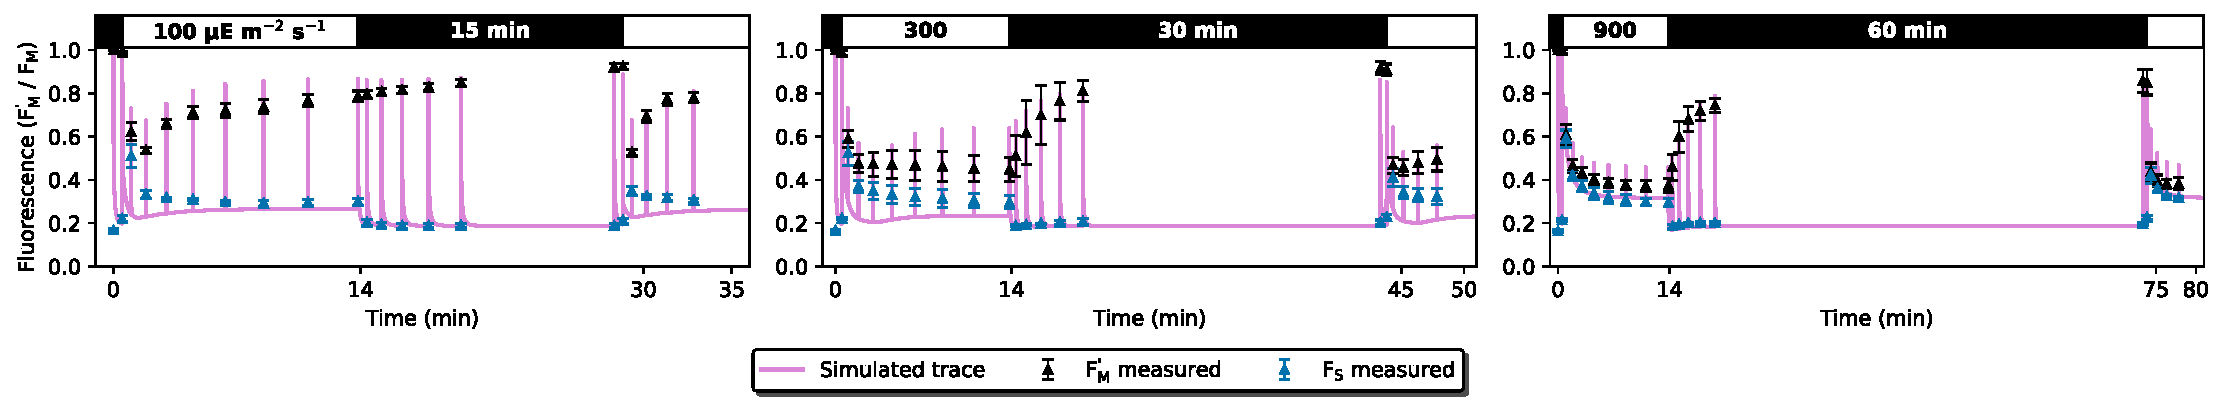
\includegraphics[width=\textwidth]{Figures/Validations/matuszynska2016_fig4.pdf}
    \captionvalid{Matuszynska2016}{Experimental and simulated \glsentryshort{pam} protocol with three different light levels and durations of \glsentrylong{arabidopsis}.}{A \glsentryfull{pam} protocol was done using \glsentrylong{arabidopsis} plants, with three different light levels and durations. The protocols start with a saturating pulse, followed by a dark period of \qty{30}{\second}, then a light period of \qty{14}{\minute} that starts with a saturating pulse and continues with 7 additional ones, all an accumulative 20 seconds apart ($+$\qty{30}{\second}, $+$\qty{50}{\second}, $+$\qty{70}{\second}, etc. from the start of the period). Then another dark period of differing lengths, also starting with a saturating pulse and going along with 5 additional ones, also an accumulative 20 seconds apart. To end the protocol, a final light period of \qty{5}{\minute}, with a saturating pulse to start and 4 additional ones, also an accumulative 20 seconds apart. The three different protocols only differ in the light intensities of the light periods and the duration of the second dark period. The first protocol, shown on the left, has a light intensity of \qty{100}{\micro\mol\per\square\meter\per\second} and a second dark period of \qty{15}{\minute}. The second protocol, shown in the middle, has a light intensity of \qty{300}{\micro\mol\per\square\meter\per\second} and a second dark period of \qty{30}{\minute}. The third protocol, shown on the right, has a light intensity of \qty{900}{\micro\mol\per\square\meter\per\second} and a second dark period of \qty{60}{\minute}. The experimental values shown, are the base \glsentryfull{F} (blue) and the \glsentryfull{Fm} (black). Three replicates for each measurement were done, but only the mean values and standard deviation are shown. The data was taken from the original publication~\cite{matuszynskaMathematicalModelNonphotochemical2016}, therefore all the other meta-information is to be read there. The simulation (pink) was done using the default parameters and changing the \glsentryfull{ppfd} to match the light intensities of the protocols and saturating pulses of \qty{2000}{\micro\mol\per\square\meter\per\second}. Additionally, the \glsentryshort{ppfd} was converted to an internal activation rate, that was calibrated to three light intensities of \glsentryshort{arabidopsis}. This was done by following equation: $\mathrm{Light} = 0.0005833 \cdot \mathrm{PPFD}^2 + 0.2667 \cdot \mathrm{PPFD} + 187.5$. This figure is recreated from figure 4 of the original publication of the Matuszynska2016 model~\cite{matuszynskaMathematicalModelNonphotochemical2016}.}
    \label{fig:matuszynska2016-fig4}
\end{figure}

The fifth figure consists of two different subfigures, the top showing a striking similarity to the publication except for the lumenal pH curve of \qty{300}{\micro\mol\per\square\meter\per\second} and \qty{900}{\micro\mol\per\square\meter\per\second} light intensity, both shifted slightly downwards in the recreation~\figref{fig:matuszynska2016-fig5}. However, both show the same trend through the time series. The phase plane trajectory on the other hand, shows only a slight similarity. The highest lumenal pH reaches at higher \gls{Q} activity is that of 7, while in the publication it is near to 8. Overall, the trajectories are all shifted downwards in the recreation, except for the trajectory of \qty{100}{\micro\mol\per\square\meter\per\second}, which shows the most similarity to the publication. On top of that, the steady-state values are also all shifted downwards and the points attributed to the light intensities, are not in the same places as in the publication.

\begin{figure}
    \centering
    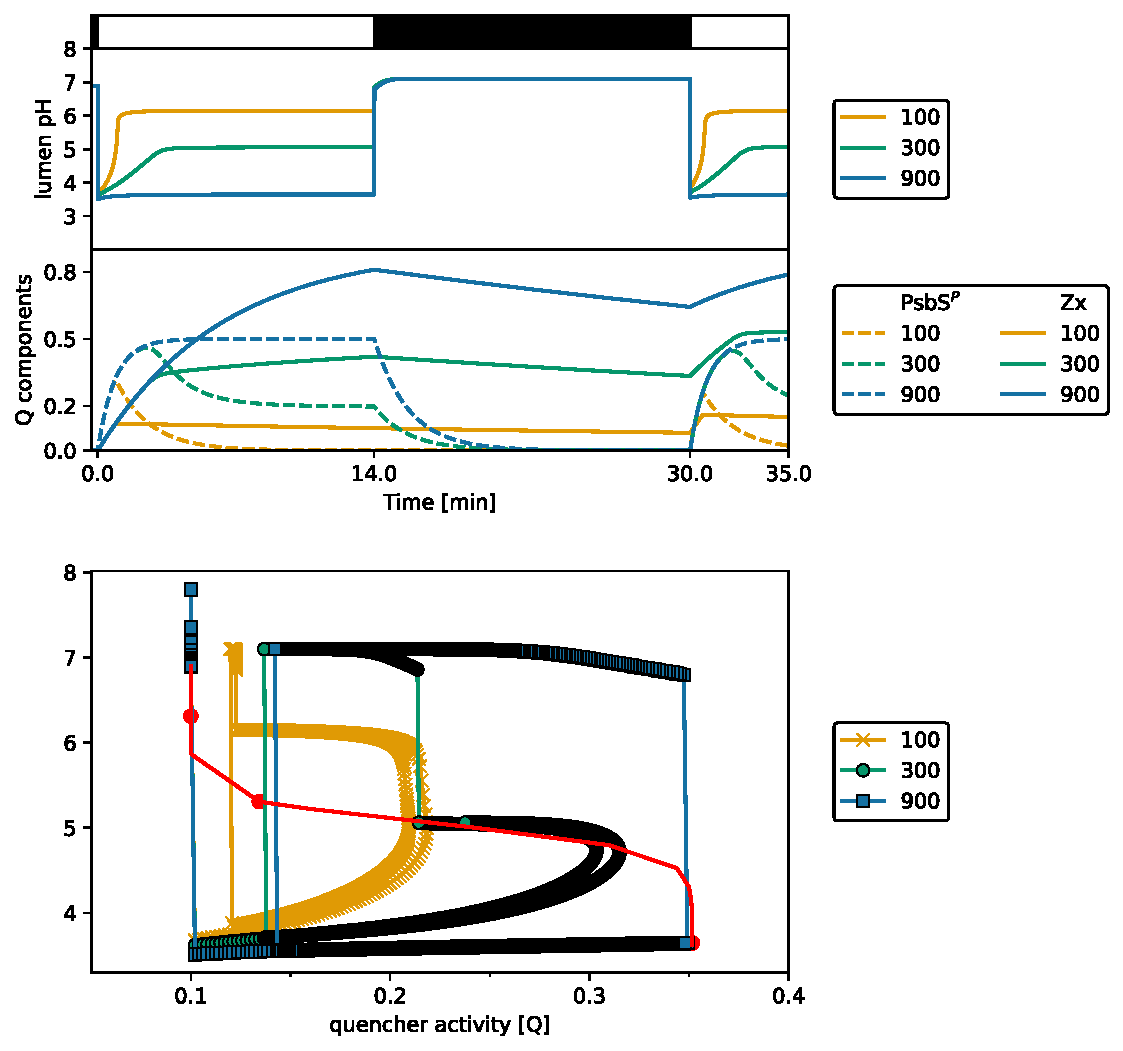
\includegraphics[width=0.7\textwidth]{Figures/Validations/matuszynska2016_fig5.pdf}
    \captionvalid{Matuszynska2016}{Visualisation of lumenal pH and quencher components in response to different light intensities.}{A protocol of dark and light periods was used to simulate the model at three different light intensities. The protocol starts with a dark period of \qty{30}{\second}, followed by a light period of \qty{14}{\minute}, then another dark period of \qty{16}{\minute}, and ending with a final light period of \qty{5}{\minute}. The three different light intensities used in the light periods were \qty{100}{\micro\mol\per\square\meter\per\second} (yellow), \qty{300}{\micro\mol\per\square\meter\per\second} (green), and \qty{900}{\micro\mol\per\square\meter\per\second} (blue). The time series of each simulation is shown in the top plot, for the lumenal pH and the concentration of the quencher components \glsentryfull{psbsp} and \glsentryfull{zx}. The bottom plot shows a phase plane trajectory of the \glsentryfull{Q} and the lumenal pH for each light intensity. Each simulation was done with the default parameters of the model, whereas the light intensities were inputted using the conversion of \glsentryfull{ppfd} to an internal activation rate for \glsentrylong{arabidopsis} by following equation: $\mathrm{Light} = 0.0005833 \cdot \mathrm{PPFD}^2 + 0.2667 \cdot \mathrm{PPFD} + 187.5$. This figure is recreated from figure 5 of the original publication of the Matuszynska2016 model~\cite{matuszynskaMathematicalModelNonphotochemical2016}.}
    \label{fig:matuszynska2016-fig5}
\end{figure}

The last figure could also be successfully recreated, with only two small discrepancies~\figref{fig:matuszynska2016-fig6}. The first is that the first value of the \gls{phipsii} curve in the recreation is much lower than in the publication and the second is that the recreation misses the last value of the \gls{phipsii} curve. Other than that, both simulation results and experimental data show a very good match to the publication. Here it should also be noted that the experimental data was shifted on the x-axis to fit the peaks of the simulation, as was done for the prior figure.

\begin{figure}
    \centering
    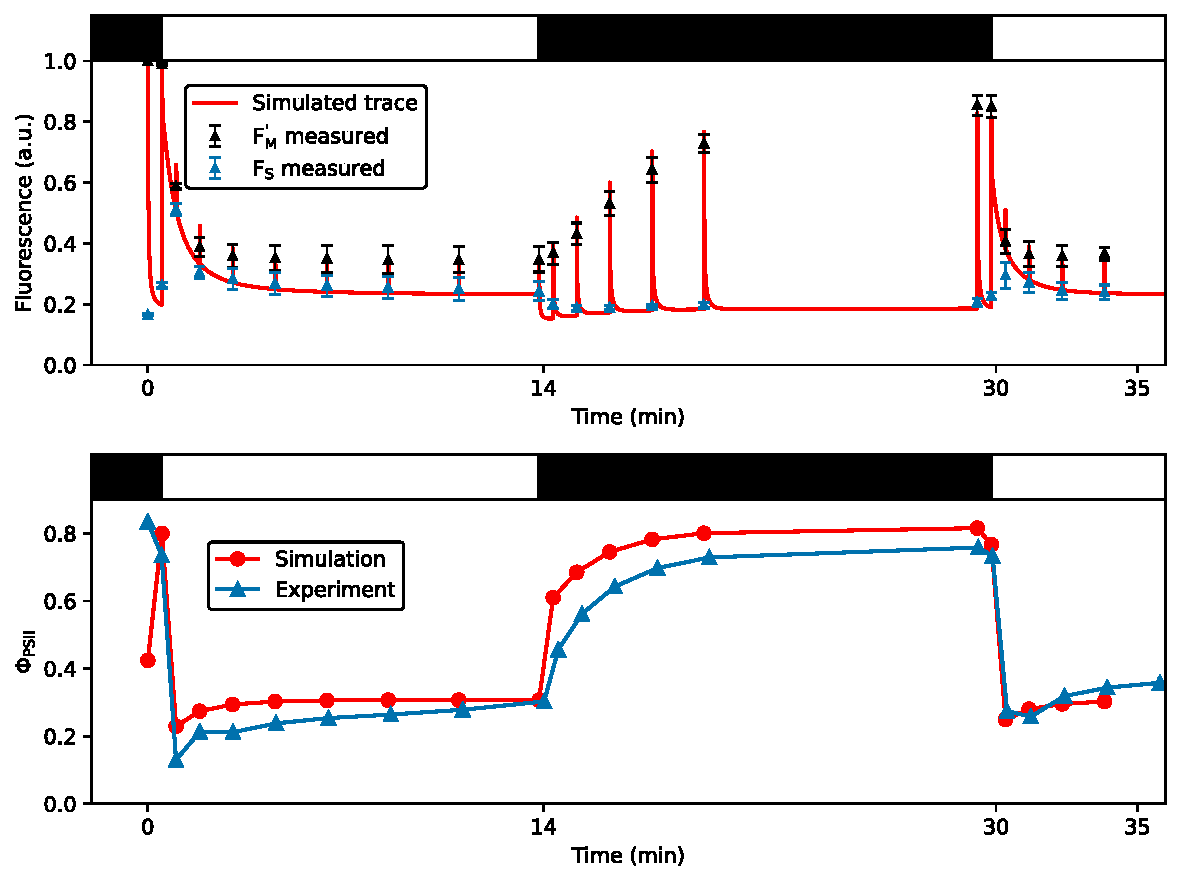
\includegraphics[width=0.7\textwidth]{Figures/Validations/matuszynska2016_fig6.pdf}
    \captionvalid{Matuszynska2016}{Experimental and simulated \glsentryshort{pam} protocol of \glsentrylong{epipremnum}.}{A \glsentryfull{pam} protocol was done using \glsentrylong{epipremnum} plants that starts with a saturating pulse, followed by a dark period of \qty{30}{\second}, then a light period of \qty{14}{\minute} of a light intensity of that starts with a saturating pulse and continues with 7 additional ones, all an accumulative 20 seconds apart ($+$\qty{30}{\second}, $+$\qty{50}{\second}, $+$\qty{70}{\second}, etc. from the start of the period). Then another dark period of \qty{16}{\minute}, also starting with a saturating pulse and going along with 5 additional ones, also an accumulative 20 seconds apart, except for the last that occurs \qty{30}{\second}. To end the protocol, a final light period of \qty{5}{\minute}, with a saturating pulse to start and 4 additional ones, also an accumulative 20 seconds apart. The light intensity used for the light periods is \qty{100}{\micro\mol\per\square\meter\per\second}, while the dark is \qty{0}{\micro\mol\per\square\meter\per\second}. The experimental values shown, are the base \glsentryfull{F} (blue) and the \glsentryfull{Fm} (black) at the top and the \glsentryfull{phipsii} at the bottom. Three replicates for each measurement were done, but only the mean values are shown and also the standard deviation for the \glsentryshort{F}. The data was taken from the original publication~\cite{matuszynskaMathematicalModelNonphotochemical2016}, therefore all the other meta-information is to be read there. To change the model to the \glsentryshort{epipremnum} version, only the \glsentryfull{gamma2} was changed ($=1$). However, the conversion of the \glsentryshort{ppfd} to an internal activation rate was done using the following equation: $\mathrm{Light} = 0.0004167 \cdot \mathrm{PPFD}^2 + 0.3333 \cdot \mathrm{PPFD} + 862.5$. With these changes the model was simulated using the same \glsentryshort{pam} protocol and the same results were plotted to the corresponding experimental data (red). This figure is recreated from figure 6 of the original publication of the Matuszynska2016 model~\cite{matuszynskaMathematicalModelNonphotochemical2016}.}
    \label{fig:matuszynska2016-fig6}
\end{figure}

\subsubsection{Saadat2021}

The second, third, fifth, and sixth figure of the Saadat2021 model~\cite{saadatComputationalAnalysisAlternative2021} were successfully recreated, without any discrepancies~(see \hyperref[fig:saadat2021-fig2]{Fig.~\ref*{fig:saadat2021-fig2}}, \hyperref[fig:saadat2021-fig3]{Fig.~\ref*{fig:saadat2021-fig3}}, \hyperref[fig:saadat2021-fig5]{Fig.~\ref*{fig:saadat2021-fig5}}, and \hyperref[fig:saadat2021-fig6]{Fig.~\ref*{fig:saadat2021-fig6}} respectively). The fourth figure, however, shows the correct trends, but the parameter range, where limit cycle oscillations of the \gls{kcyc} parameter were observed, could not be recreated. This issue made it therefore impossible to fully recreate the figure, which is why the lines in the recreation are much more jagged than in the publication~\figref{fig:saadat2021-fig4}.

\begin{figure}
    \centering
    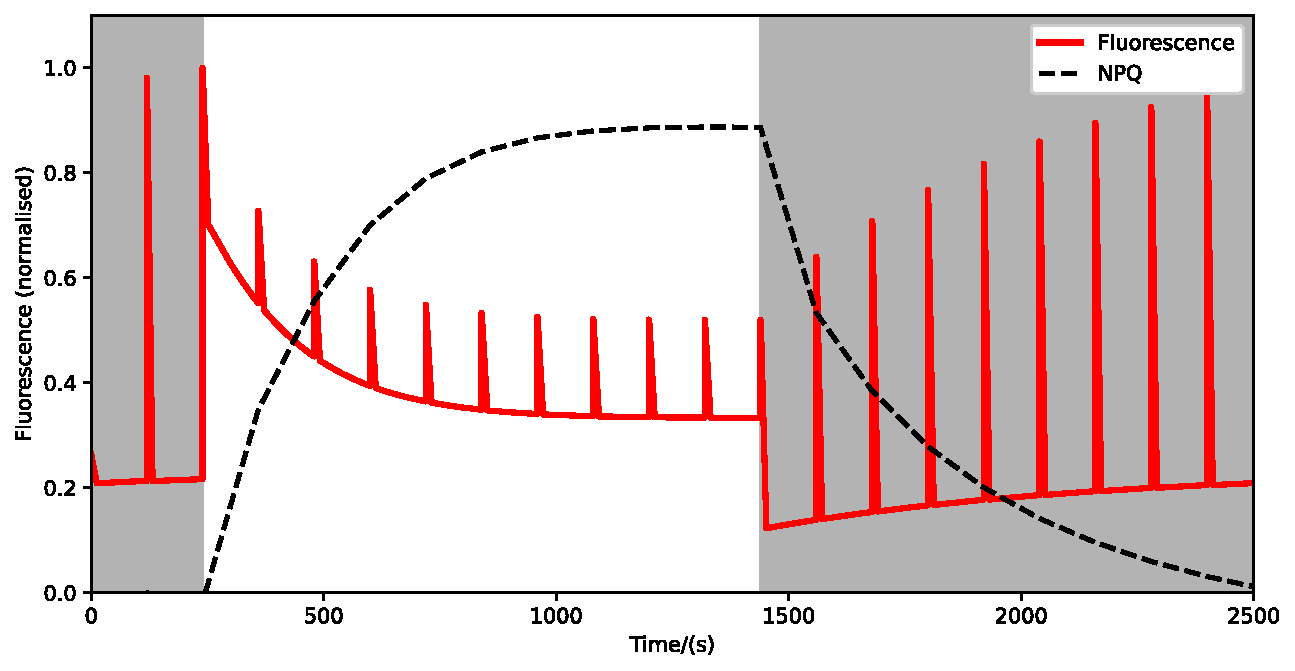
\includegraphics[width=0.7\textwidth]{Figures/Validations/saadat2021_fig2.pdf}
    \captionvalid{Saadat2021}{Results of a generic \gls{pam} protocol.}{The generic \glsentryfull{pam} protocol starts with a \qty{4}{\minute} dark period with a saturating pulse at the \qty{2}{\minute} mark. At the end of the dark period, another saturating pulse indicates the start of an actinic light period that goes on for \qty{10}{\minute}, with saturating pulses every \qty{2}{\minute}. Then another dark period of \qty{18}{\minute} starts, again with a saturating pulse at the start and at each \qty{2}{\minute} mark. The light intensity used for the actinic light period is \qty{1000}{\micro\mol\per\square\meter\per\second}, while the dark periods are \qty{40}{\micro\mol\per\square\meter\per\second}. Each saturating pulse was simulated for \qty{0.8}{\second} at a light intensity of \qty{5000}{\micro\mol\per\square\meter\per\second}. The simulation is run using the default parameters and initial conditions of the model, except for the \glsentryfull{kcyc} ($=0$) to match an organism with no cyclic electron flow. The values of light intensity were inputted directly to the \glsentryfull{ppfd} parameter of the model. The results shown are the \glsentryfull{F} which was normalized to the maximum value of that series (red), and the \glsentryfull{npq} (black), which was calculated by using the \glsentryshort{F} and \glsentryfull{Fm}~\cleverref{Eq.}{eq:npq}. This figure is recreated from figure 2 of the original publication of the Saadat2021 model~\cite{saadatComputationalAnalysisAlternative2021}.}
    \label{fig:saadat2021-fig2}
\end{figure}

\begin{figure}
    \centering
    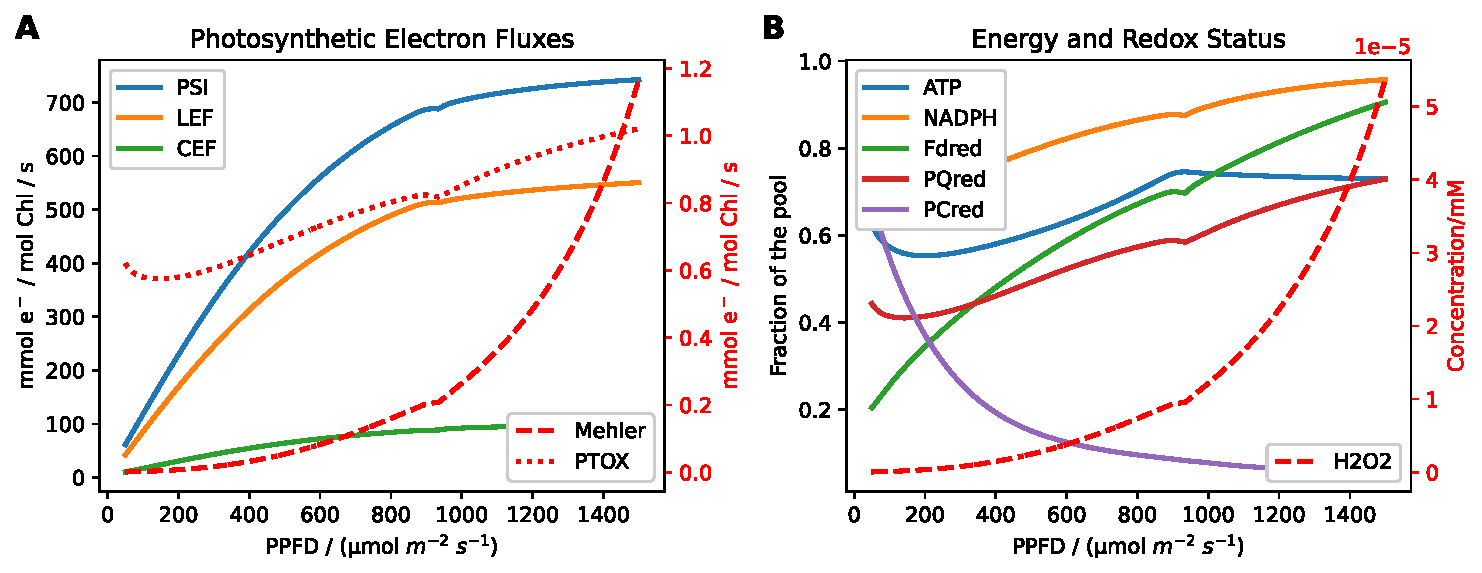
\includegraphics[width=0.7\textwidth]{Figures/Validations/saadat2021_fig3.pdf}
    \captionvalid{Saadat2021}{Results of a steady-state scan of \glsentryshort{ppfd}.}{The model was simulated to steady-state under different \glsentryfull{ppfd} values, ranging from \qty{50}{\micro\mol\per\square\meter\per\second} to \qty{1500}{\micro\mol\per\square\meter\per\second}. The results are separated in two different plots, differentiating between photosynthetic electron fluxes and the energy and redox status. The left side shows the \glsentryfull{vpsi} (blue), the \glsentryfull{lef} (orange, and calculated by doubling the \glsentryfull{vpsii}), the \glsentryfull{vcyc} (green), the \glsentryfull{vmehler} (red and dashed), and the \glsentryfull{vptox} (red and dotted). On the right side the ratios of \glsentryfull{atp} (blue), \glsentryfull{nadph}  (orange), \glsentryfull{fdred} (green), \glsentryfull{pqred} (red), and \glsentryfull{pcred} (purple) to their total pools are shown. Additionally the concentration of \glsentryfull{h2o2} (red, dashed) is also plotted. The simulation is run using the default parameters and initial conditions of the model, while changing only the \glsentryfull{ppfd} to the desired value for each simulation. This figure is recreated from figure 3 of the original publication of the Saadat2021 model~\cite{saadatComputationalAnalysisAlternative2021}.
    }
    \label{fig:saadat2021-fig3}
\end{figure}

\begin{figure}
    \centering
    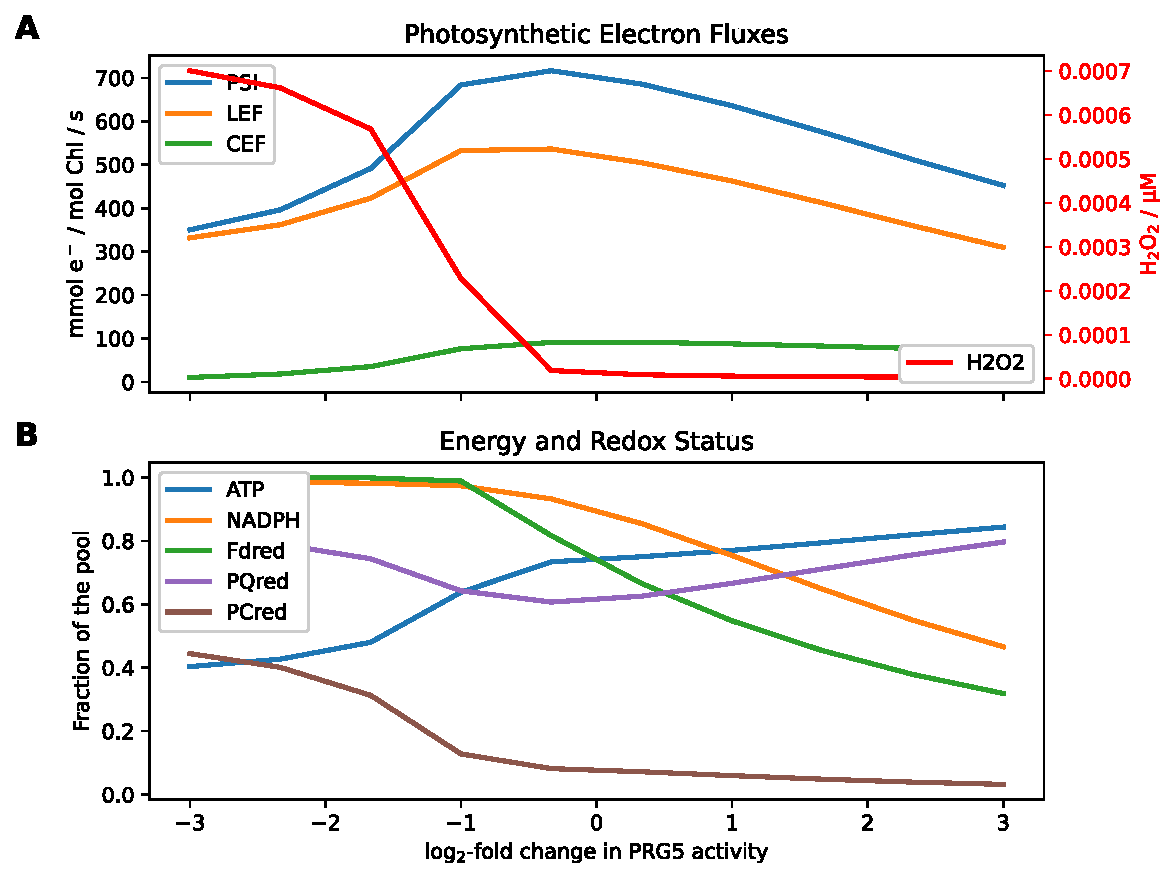
\includegraphics[width=0.7\textwidth]{Figures/Validations/saadat2021_fig4.pdf}
    \captionvalid{Saadat2021}{Results of a steady-state scan of aletered \glsentryshort{cef}.}{The model was simulated to steady-state under different \glsentryfull{kcyc} values representing $\log_2$-fold changes ranging from negative three to three. The results are separated in two different plots, differentiating between photosynthetic electron fluxes and the energy and redox status. The top plot shows the \glsentryfull{vpsi} (blue), the \glsentryfull{lef} (orange, and calculated by doubling the \glsentryfull{vpsii}), the \glsentryfull{vcyc} (green), and the concentration of \glsentryfull{h2o2} (red). In the bottom plot the ratios of \glsentryfull{atp} (blue), \glsentryfull{nadph}  (orange), \glsentryfull{fdred} (green), \glsentryfull{pqred} (red), and \glsentryfull{pcred} (purple) to their total pools are shown. The simulation is run at a \glsentryfull{ppfd} of \qty{1000}{\micro\mol\per\square\meter\per\second}, otherwise using the default parameters and initial conditions of the model, while changing only the \glsentryshort{kcyc} to the desired value for each simulation. Due to issues of singular ranges of \glsentryshort{kcyc} not being able to be simulated to steady-state, only a few values could actually be plotted, to bee seen by the jaggedness of the lines. This figure is recreated from figure 3 of the original publication of the Saadat2021 model~\cite{saadatComputationalAnalysisAlternative2021}.}
    \label{fig:saadat2021-fig4}
\end{figure}

\begin{figure}
    \centering
    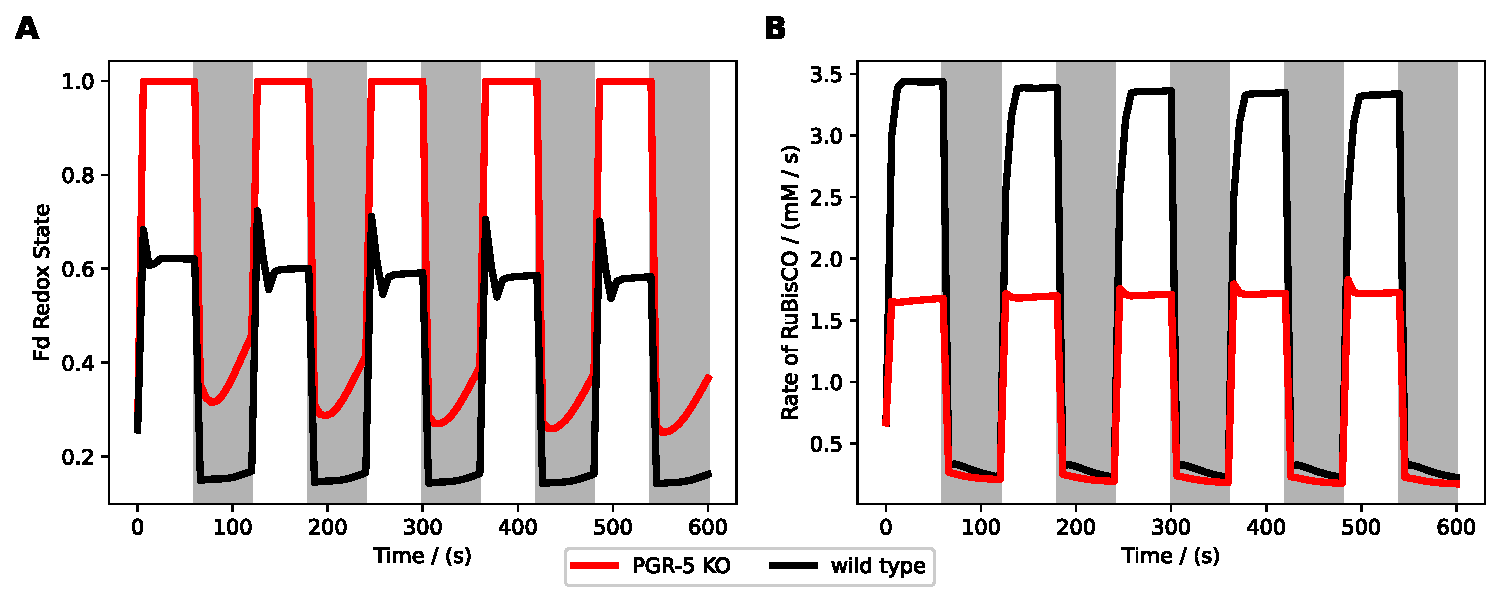
\includegraphics[width=0.7\textwidth]{Figures/Validations/saadat2021_fig5.pdf}
    \captionvalid{Saadat2021}{Comparison of results of a wildtype and knockout mutant simulation under varying light intensities.}{A simple fluctuating light protocol was used to simulate a wildtype (black) and a knockout mutant (red) of the model. The protocol undergoes a total of 10 periods, each of them lasting \qty{1}{\minute}. The light intensities of the periods alternate between light and dark, using a light intensity of \qty{600}{\micro\mol\per\square\meter\per\second} and \qty{40}{\micro\mol\per\square\meter\per\second}, respectively. The wildtype simulation was run using the default parameters and initial conditions of the model, while the knockout mutant was simulated by setting the \glsentryfull{kcyc} to zero. Each light intensity was inputted into the \glsentryfull{ppfd} parameter of the models. The results shown are the ratio of \glsentryfull{fdred} to its total pool on the left, and the \glsentryfull{vc} on the right. This figure is recreated from figure 5 of the original publication of the Saadat2021 model~\cite{saadatComputationalAnalysisAlternative2021}.}
    \label{fig:saadat2021-fig5}
\end{figure}

\begin{figure}
    \centering
    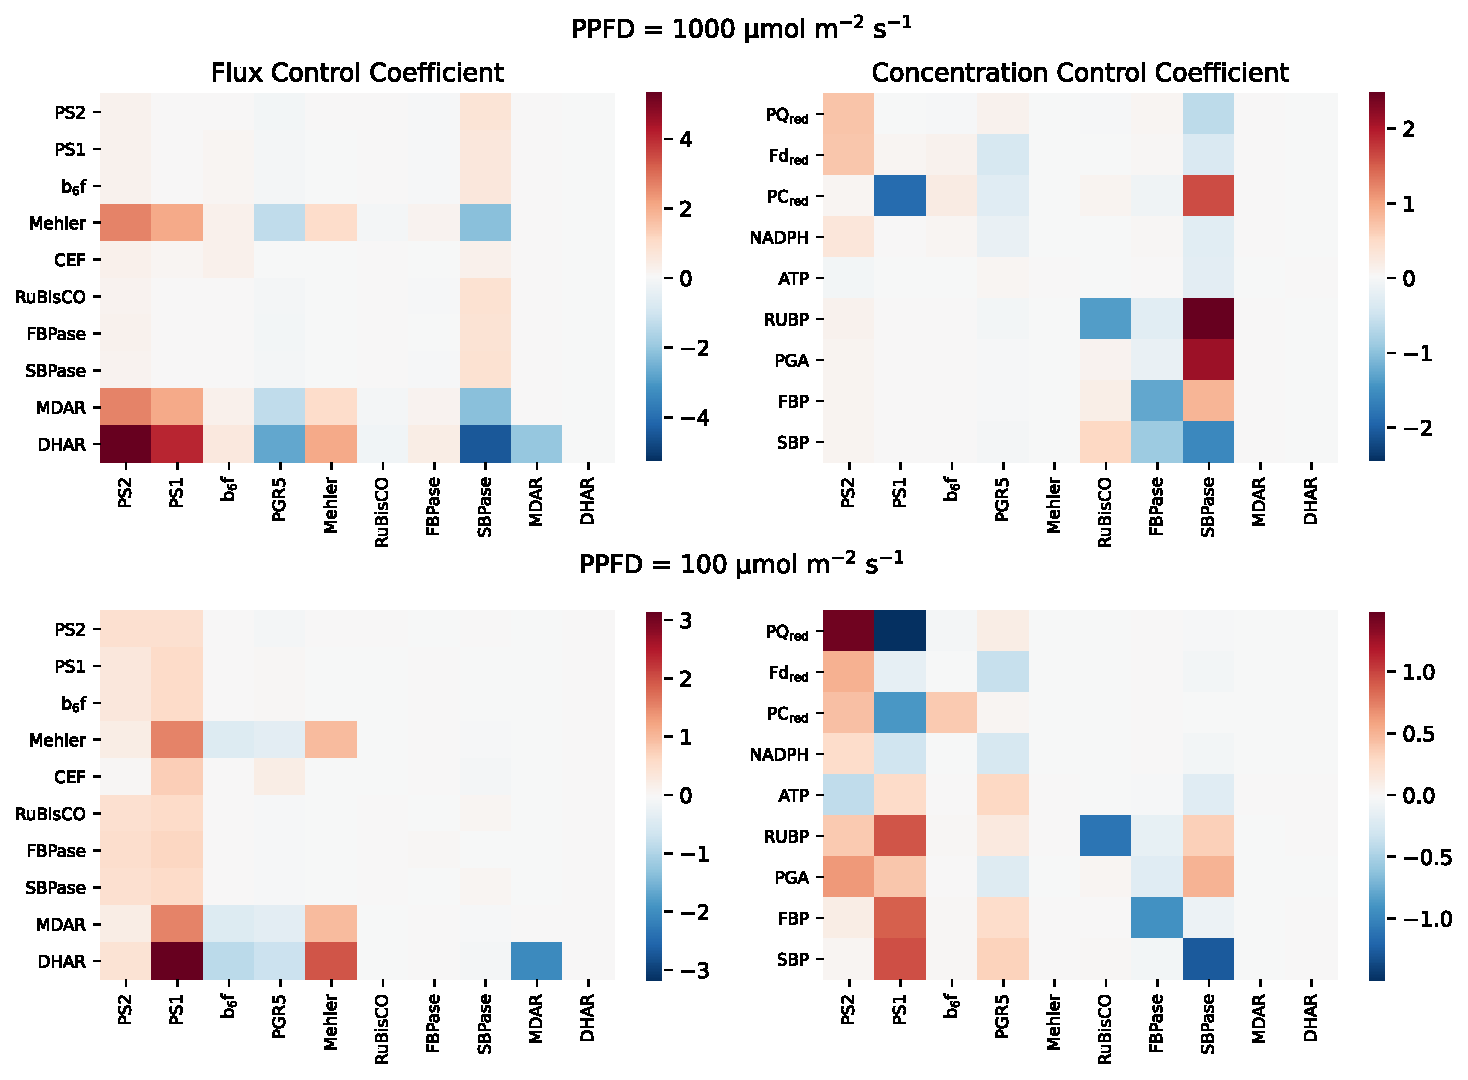
\includegraphics[width=0.7\textwidth]{Figures/Validations/saadat2021_fig6.pdf}
    \captionvalid{Saadat2021}{\glsentryshort{mca} of key aspects of the model under two different light intensities.}{A \glsentryfull{mca} was done to the model under two different light intensities, \qty{1000}{\micro\mol\per\square\meter\per\second} (top) and \qty{1000}{\micro\mol\per\square\meter\per\second} (bottom). The results of the fluxes can be found on the left, while on the right are the variables. The parameters that were used for the \glsentryshort{mca} are the control coefficients of the fluxes with the same names. The following were used, given from left to right on the x-axis of each heatmap: \glsentryfull{psiitot}, \glsentryfull{psitot}, \glsentryfull{kcatb6f}, \glsentryfull{kcyc}, \glsentryfull{kmehler}, \glsentryfull{kcatvc}, \glsentryfull{kcatfbpase}, \glsentryfull{kcatsbpase}, \glsentryfull{kcatmdareduct}, and \glsentryfull{kcatdhar}. These parameters were displaced by $\pm 1\%$. The simulations were otherwise done using the default parameters and initial conditions of the model, while changing only the \glsentryfull{ppfd} to the desired value for each simulation. This figure is recreated from figure 6 of the original publication of the Saadat2021 model~\cite{saadatComputationalAnalysisAlternative2021}.
    }
    \label{fig:saadat2021-fig6}
\end{figure}

The last figure of the publication includes the same parameter range as the fourth figure, therefore the same issue is observed in the recreation. However in this case, the recreation could not be completed at all, as the specific range of the \gls{kcyc} parameter where these oscillations are found is not well documented.

\subsection{Model Demonstrations}

\subsubsection{Daylight Simulation}

The light intensity during the chosen day period follows an approximate bell curve, common for these sorts of graphs. As sunlight is not a constant source, but may change dynamically due to weather conditions, the light intensity shows simple peaks and valleys during the entire day. This allows to test the capabilities of the models to simulate complex and dynamic light protocols, which is a common issue for many models. In this case, all but the Li2021 model show results to varying degree~\figref{fig:daylight-demon}.

The Bellasio2019 model shows a clear response to the changing light conditions, both the \gls{vc} and the \gls{atp} and \gls{nadph} ratio rising and falling with the light intensity during the day. However, at approximately 10:30, both reach a plateau, that goes on until approximately 16:00, where the light intensity begins to fall. There the \gls{vc} slowly begins to fall to 0 until the end of the simulation, while the \gls{atp} and \gls{nadph} ratio slowly rises until 18:00 and then falls following the pattern of the \gls{vc} line. As this model does not have a quantity representing \gls{F}, it cannot be plotted.

The Fuente2024 model only has a representative quantity for \gls{F}, which follows the light intensity pattern very closely. However, in the moments of lower light, the \gls{F} values are more sensitive to the light fluctuations, as for example the peak at 08:00 causes the \gls{F} to rise to the same values as during the highest light intensities. Additionally, the \gls{F} values show a small rise when the day begins to end, which does not follow the light intensity pattern. However, in the higher light intensities, the \gls{F} values do follow the light intensity pattern very closely.

The Matuszynska2016 model, also only shows a representative quantity for \gls{F}, which also follows the light intensity pattern very closely. Just like with the Fuente2024 model, the \gls{F} values follow the light pattern closest during the higher light intensities, while during the lower light intensities, they are more sensitive to the light fluctuations. Interestingly, this model also shows a small rise in \gls{F} values when the day begins to end.

The Saadat2021 model shows all three representative quantities, \gls{vc}, \gls{atp} and \gls{nadph} ratio, and \gls{F}. The \gls{vc} values show a clear correlative response to the light intensity, rising and falling with the light intensity during the day. Comparatively to the Bellasio2019 model, these values also reach a plateau at 10:30 and slowly fall after 16:00. Contrary to the other models though, both the \gls{atp} and \gls{nadph} ratio, and the \gls{F} values show an anticorrelative response to the light intensities. Especially the \gls{F} which drops significantly during the higher light intensities, while rising during the lower light intensities. It also reaches a plateau at 10:30, but then slowly rises at 16:00, to reach approximately the same starting value as of the start of the day. The \gls{atp} and \gls{nadph} ratio also shows a similar pattern, but with less significant changes.

\begin{figure}
    \centering
    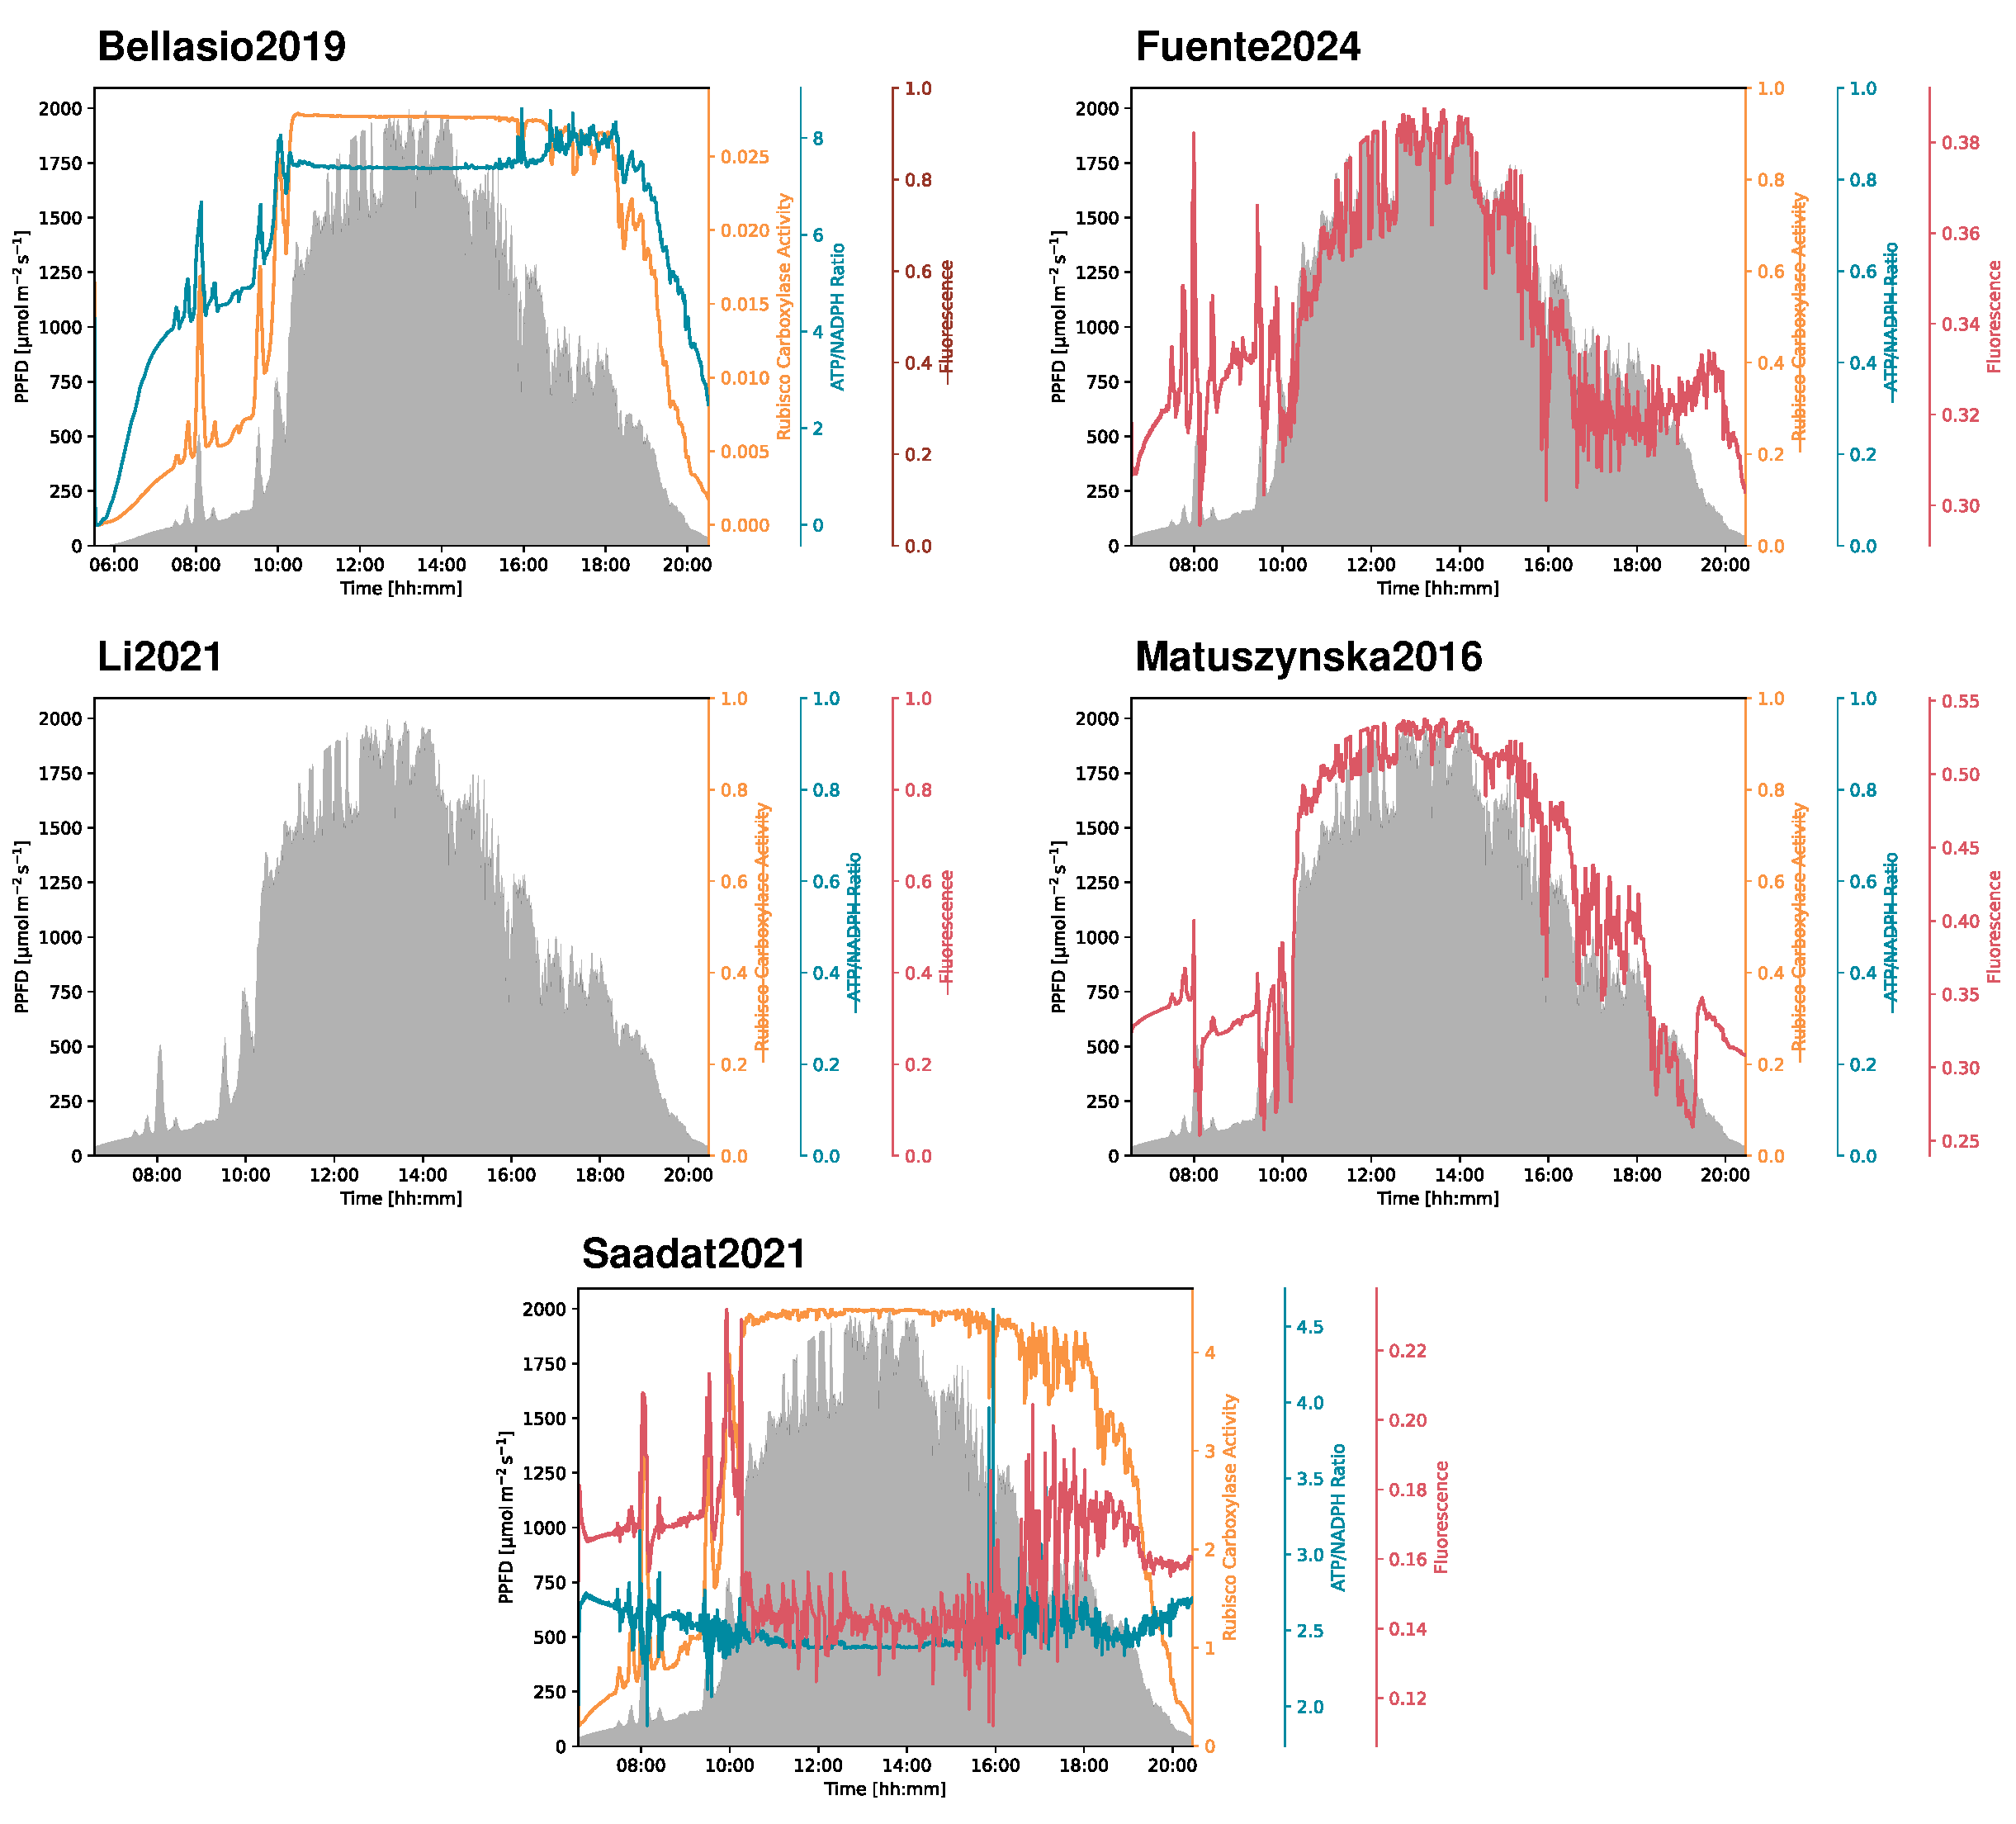
\includegraphics[width=0.7\textwidth]{Figures/Demonstrations/daysimulation.pdf}
    \captionprof{Combined Daylight Simulation demonstrations of all models.}{Sample simulation of a day cycle using real \glsentryfull{ppfd} data from Kansas, USA on June 19, 2023. The data was obtained from the \glsentryfull{neon} data portal~\cite{nationalecologicalobservatorynetworkneonPhotosyntheticallyActiveRadiation2023} and is used to create a protocol for the light intensity \glsentryshort{ppfd} over the course of the day, in a minute interval. The data used is filtered to only show a \glsentryshort{ppfd} that equals or is higher than \qty{40}{\micro\mol\per\square\meter\per\second}. This threshold is chosen as it has shown to allow most models to still simulate the photosynthetic machinery, while still being a decent representation of the actual daylight conditions. The simulation is run using the default parameters and initial conditions of each model, and the \glsentryfull{vc}, \glsentryfull{atp} and \glsentryfull{nadph} ratio, and \glsentryfull{F} results is plotted over the course of the day, if possible. The results do not represent actual plant behavior, but show the capabilities of the model to simulate complex and more realistic light protocols.} 
    \label{fig:daylight-demon}
\end{figure}

\subsubsection{FvCB Add-on}

Only the Bellasio2019 and Saadat2021 models have a successful demonstration of the \gls{fvcb} add-on, as the other models do not have the required quantities'~\figref{fig:fvcb-demon}. The Fuente2024, Li2021 and Matuszynska2016 models all do not include a representation for \gls{vc} and \gls{co2}. Without these, a \gls{fvcb} style assimilation could not be calculated.

The Bellasio2019 on the other hand, shows a very distinct correlation between the simulation results and the min-W \gls{fvcb} model, with general parameters used~\cite{lochockiWidelyUsedVariants2025a}. However, once the simulation is done at higher \gls{ci} values, both the \gls{vc} and \gls{A} values drop below the \gls{fvcb} model. On top of that, they are small divots in the simulation results, which may be resulted in an unsuccessful steady-state analysis, and therefore an automatic rescue to a quasi-steady-state, \qty{1800}{s}, was performed.

The Saadat2021 model results have approximately the same shape of curve than the \gls{fvcb} model, but the ascent is much steeper. This can be seen, by the \gls{A} of the Saadat2021 model beginning lower but ending higher than the \gls{fvcb} \gls{A}. Both of the \gls{vc} start at the same point, namely \qty{0}{\micro\mol\per\meter\squared\per\second}, but the Saadat2021 model also reaches a higher value.

\begin{figure}
    \centering
    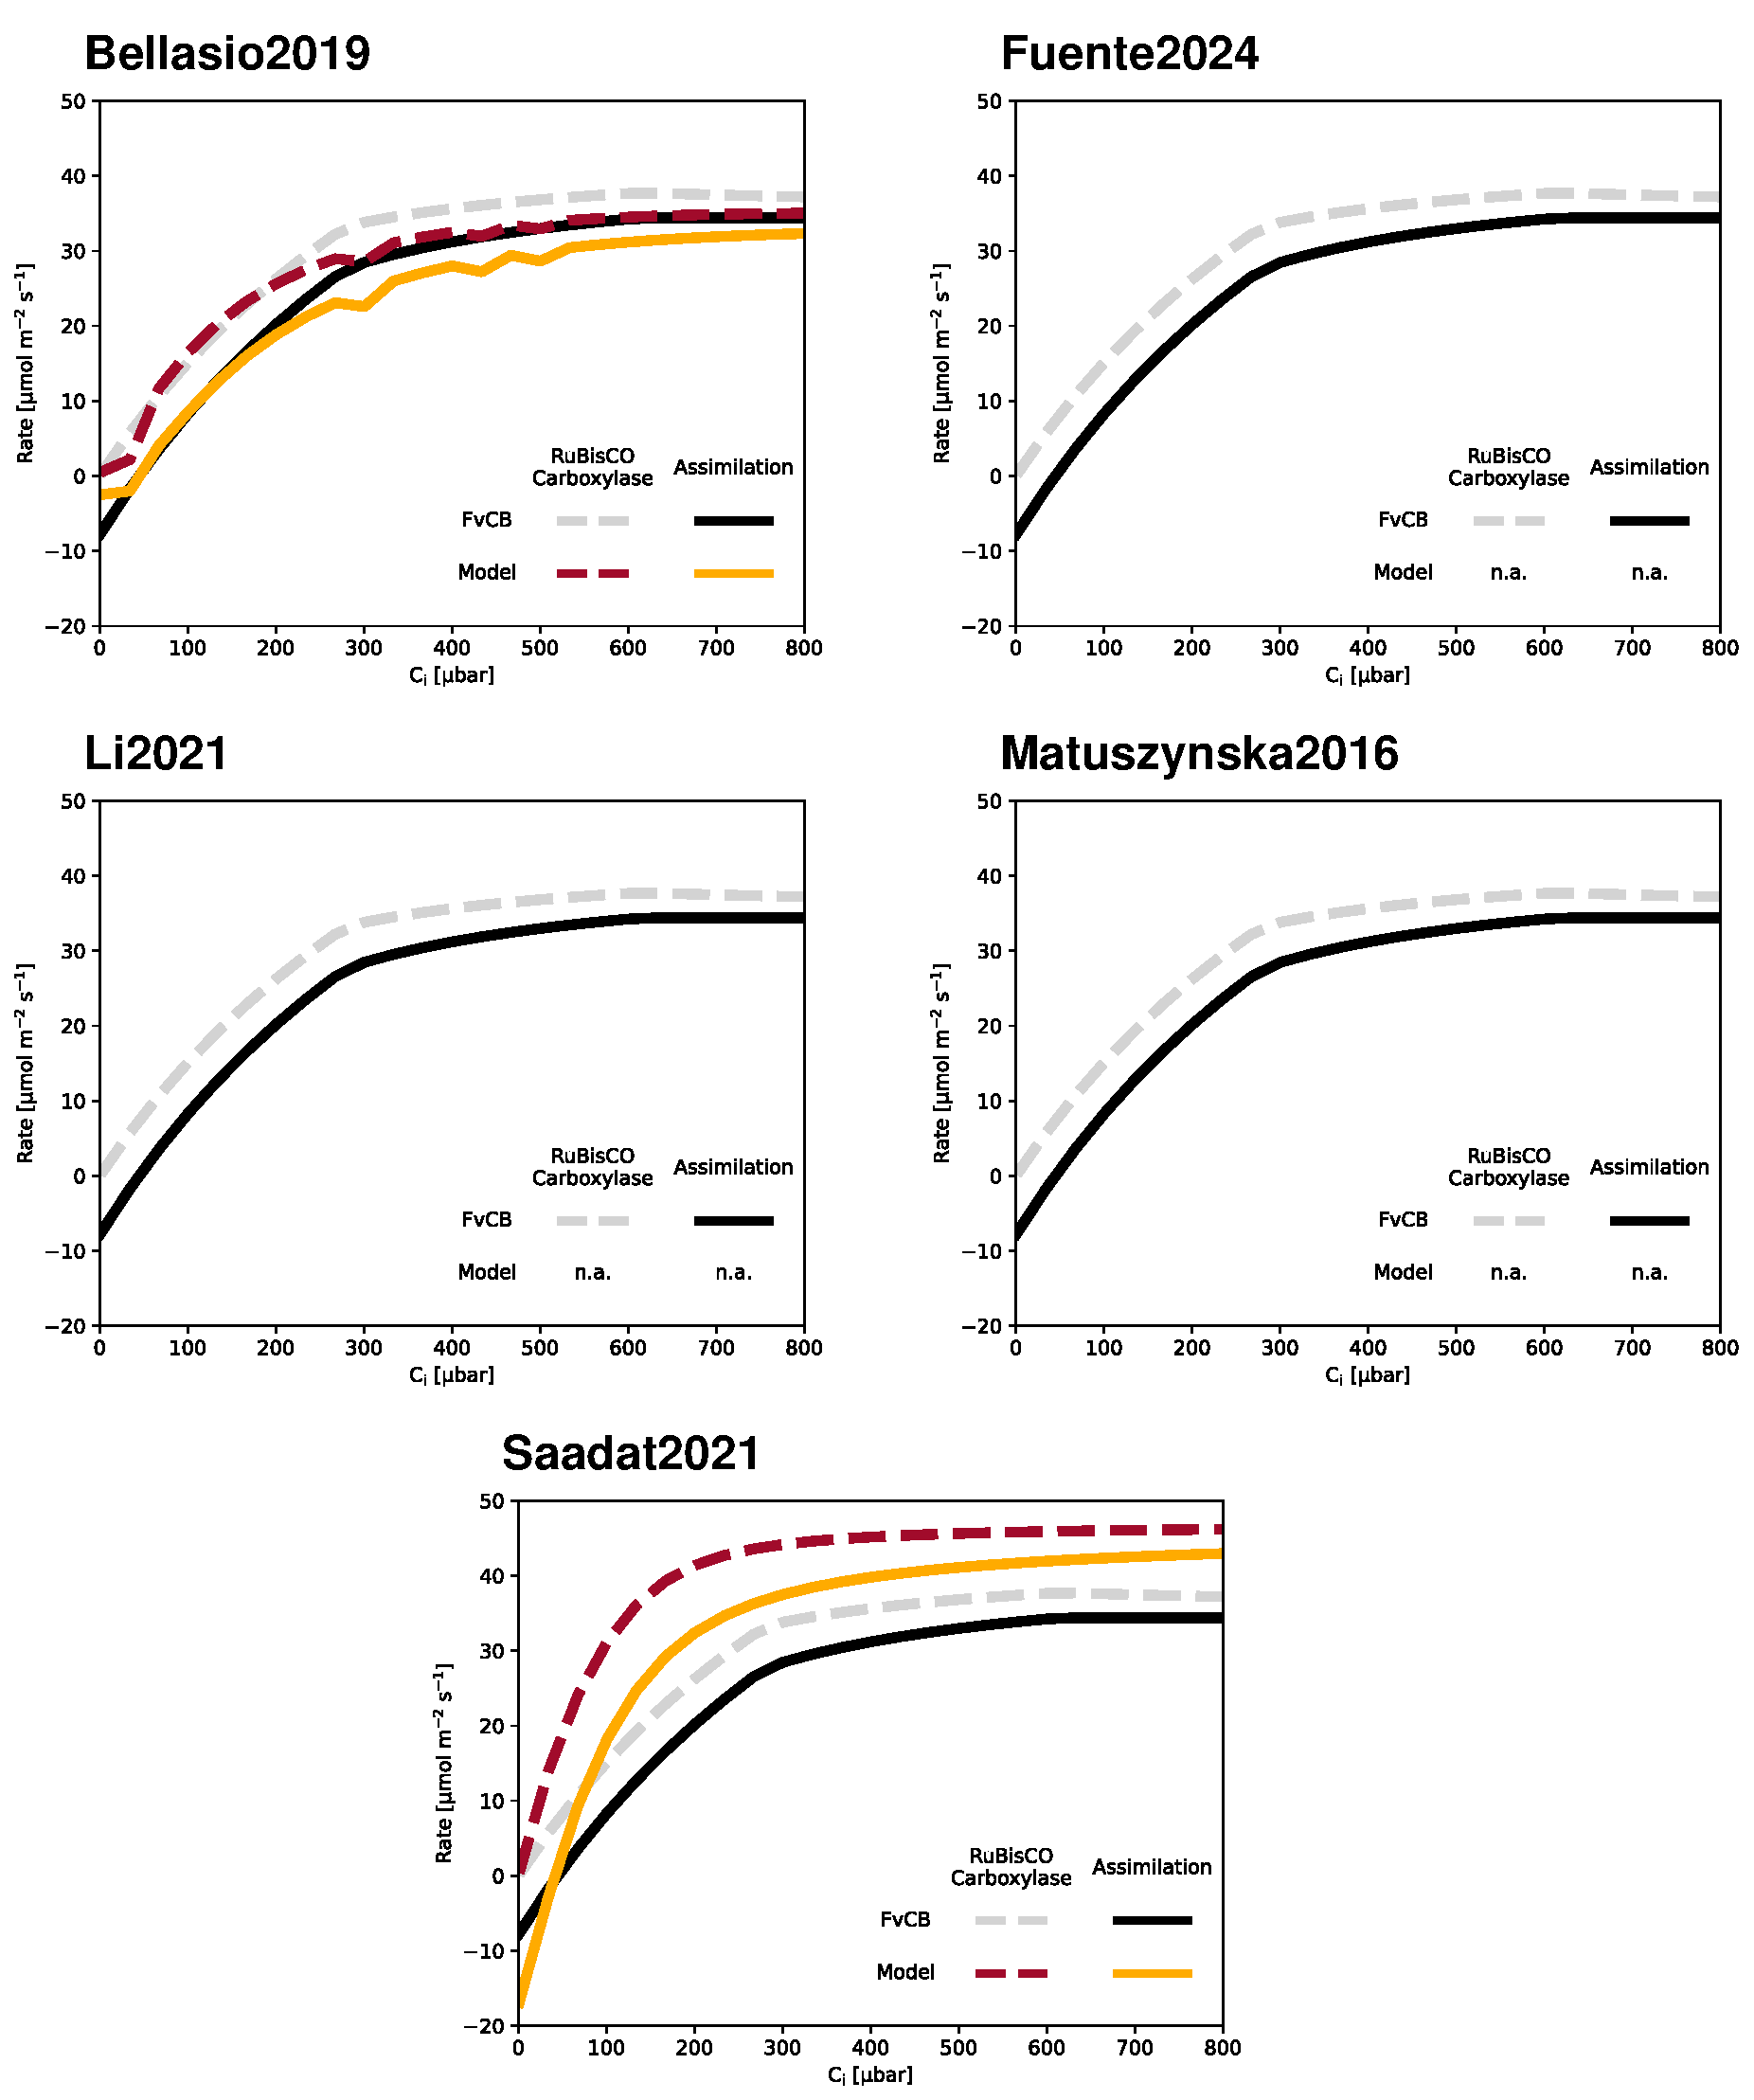
\includegraphics[width=0.7\textwidth]{Figures/Demonstrations/fvcb.pdf}
    \captionprof{Combined FvCB Addon demonstrations of all models.}{Comparison of modelled \glsentryfull{A} and \glsentryfull{vc} against the \glsentryfull{fvcb} model. The \glsentryshort{fvcb} model is calculated using the min-W approach as described by Lochoki and McGrath (2025)~\cite{lochockiWidelyUsedVariants2025a}. To be able to simulate \glsentryshort{A}, there are two mandatory quantities that need to be present in the model: \glsentryfull{co2} concentration and \glsentryshort{vc}. If one of these parameters is missing, the \glsentryshort{fvcb} model will still be shown, but no comparison with the model will be possible. Other parameters that are required to calculate the \glsentryshort{fvcb} model will be added as parameters with default values if they are not present in the model. The simulation is then run until steady-state, or quasi-steady-state if not otherwise possible, for different \glsentryfull{ci} partial pressure. The carbon assimilation shown does not represent actual values but rather a theoretical curve to compare the kinetic model to the popular \glsentryshort{fvcb} model.} 
    \label{fig:fvcb-demon}
\end{figure}

\subsubsection{Standard PAM Simulation}

All models show a successful demonstration of the standard \gls{pam} simulation~\figref{fig:pam-demon}, except the Bellasio2019 model, which does not have a quantity representing \gls{F} nor \gls{npq}. Additionally, the Li2021 model only includes a quantity for \gls{npq}, which shows a typical curve of \gls{npq} for the standard protocol. However, at the start of the protocol, an uncommon small peak can be seen, with a slow ascent and descent. Due to the fact, that the model does not contain a quantity for \gls{F}, it is harder to see the different points of time when a saturating pulse was used. Still, due to the continuous simulation of the \gls{npq}, the curve is much smoother than the other models, and small spikes can be seen that can be attributed to time points of saturating pulses.

The Fuente2024, Matuszynska2016, and Saadat2021 models all follow the typical pattern for \gls{F} a \gls{pam} protocol. The \gls{F} values starting relatively high after the dark adaptation period, with the \gls{Fm} at saturating pulses being the highest in the first dark period. Then the base \gls{F} values stay stagnant during the actinic light period, where they are higher than during the prior dark period for the Fuente2024 and Matuszynska2016 models, but lower for the Saadat2021 model. In the same light period, the \gls{Fm} values quickly drop to a lower and stable value in all three models. Then during the second dark period for all three models, the base \gls{F} values drop even lower than in the first dark period, but slowly rising back following the simulation time. The \gls{Fm} values all gradually rise during the second dark period, but do not reach the same values as during the first period.

The \gls{npq} curves of all three models also follow a typical pattern, with them start at near 0 in the first dark period, then quickly rising to a stable value in a curve during the actinic light period. Only the Saadat2021 model, shows a \gls{npq} curve in the actinic light period that reaches over its stagnating point at the start. However, then all three models show a curved drop during the second dark period, reaching a stable value that is higher than at the starting point. As the Matuszynska2016 and Saadat2021 models do not have a quantity for \gls{npq}, it had to be calculated using \gls{F} and \gls{Fm}~\cleverref[]{Equation}{eq:npq}, meaning the amount of points for the \gls{npq} curves is the same as the number of \gls{Fm} present in the simulation. This creates a more jagged curve, while the Fuente2024 model, which has a quantity for \gls{npq}, shows a smoother curve.

\begin{figure}
    \centering
    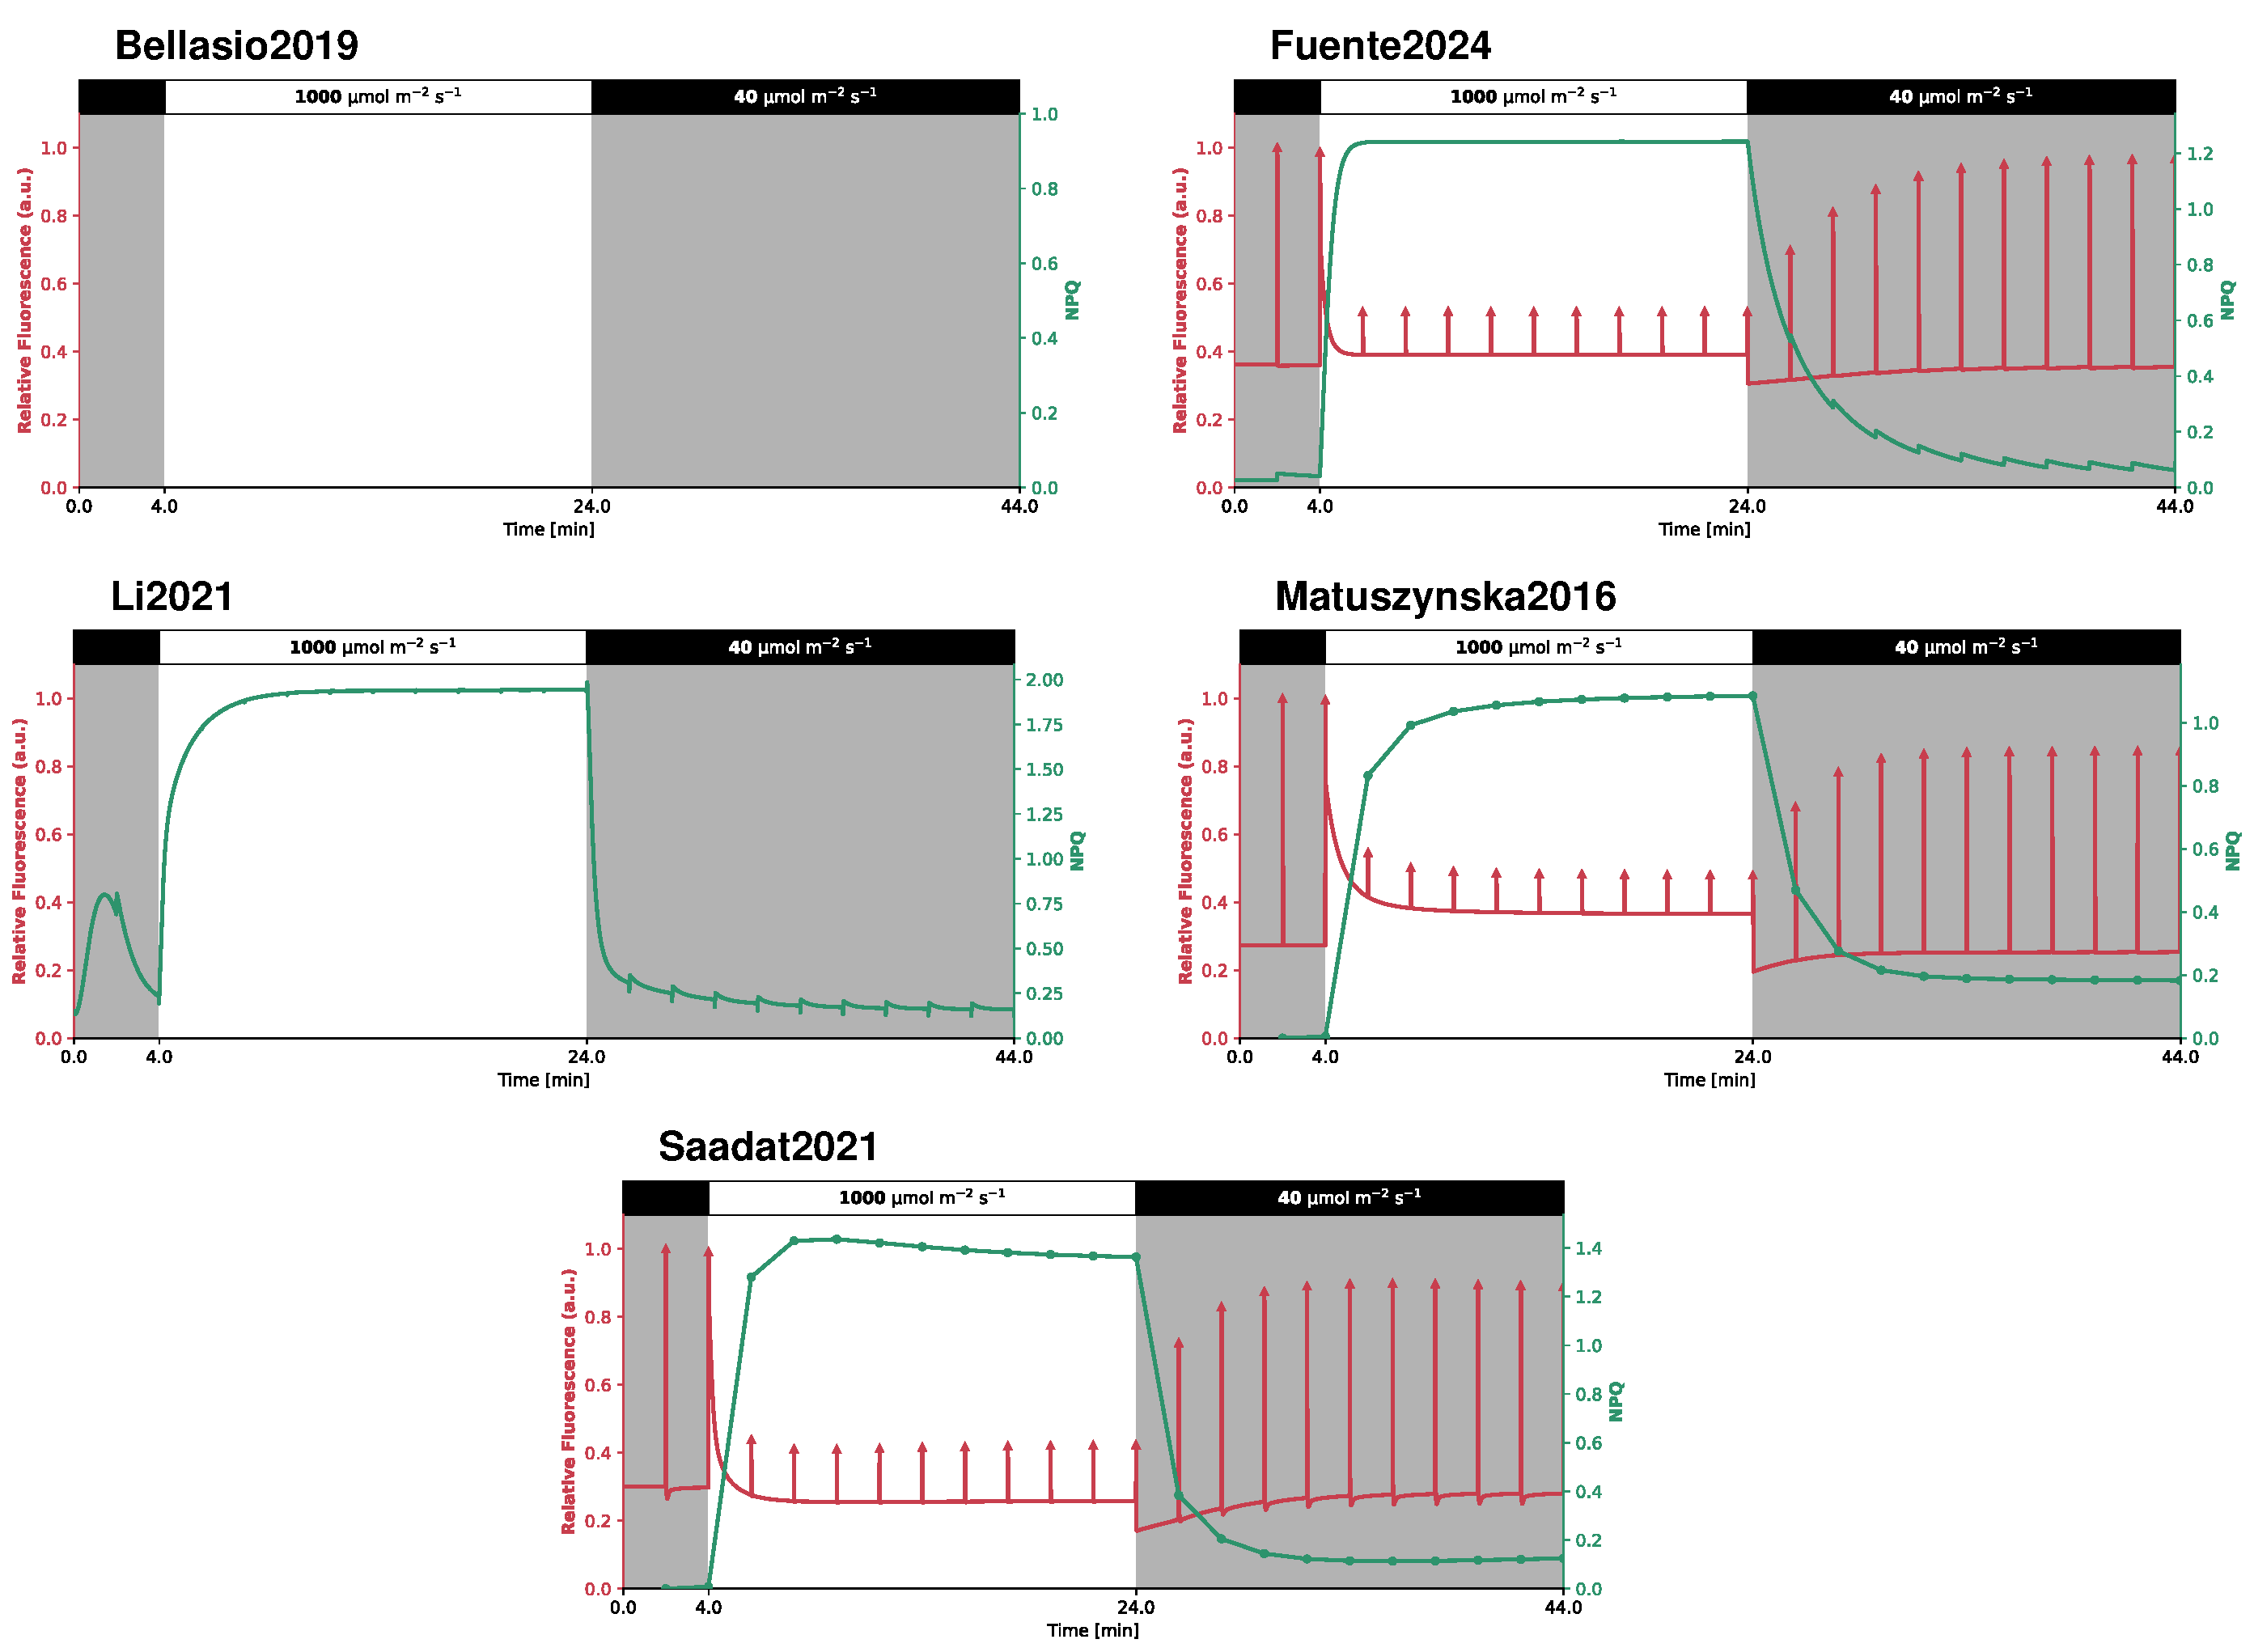
\includegraphics[width=0.7\textwidth]{Figures/Demonstrations/pam.pdf}
    \captionprof{Combined PAM Simulation demonstrations of all models.}{Sample simulation of a common \glsentryfull{pam} protocol to show fluctuations of \glsentryfull{F} and \glsentryfull{npq} using saturating pulses. The simulation protocol is as follows: A dark adaptation period that simulates for 30 minutes at a dark light intensity (\qty{40}{\micro\mol\per\square\meter\per\second}), then the actual protocol starts. The protocol consists of 22 periods with each being 2 minutes of length. That period consists of a specific light intensity of the respective type of period and ends with a saturating pulse with a length of \qty{0.8}{s} and a light intensity of \qty{3000}{\micro\mol\per\square\meter\per\second}. First, two dark periods with light intensity of \qty{40}{\micro\mol\per\square\meter\per\second}, followed by ten light periods with light intensity of \qty{1000}{\micro\mol\per\square\meter\per\second}, then ten dark periods again. The simulation is run using the default parameters and initial conditions of each model.}
    \label{fig:pam-demon}
\end{figure}

\subsubsection{MCA of Photosynthesis}

No models could complete the entire \gls{mca} heatmaps, neither the variables nor the fluxes~\figref{fig:mca-demon}. On top of that, the Li2021 shows completely empty heatmaps, even though it has some of the required quantities to perform the \gls{mca}. This is due to the model not being able to achieve steady-state for the parameters scanned, which is required for a \gls{mca} analysis on control coefficients.

The Bellasio2019 model shows results for the control coefficients of \gls{psii} and \gls{rubisco} for \gls{rubp}, \gls{co2}, \gls{atp}, and \gls{nadph} for the variables, and \gls{vc}, and \gls{vatp} for the fluxes. Both control coefficients do not have much control on the variables, except for the \gls{rubisco} coefficient on \gls{rubp}, which shows a strong negative control. On the fluxes side, both coefficients do not show much control on both \gls{vc} and \gls{vatp}.

The Fuente2024 model only shows results for the control coefficients of \gls{psii} and \gls{psi} for \gls{pq_ox}, \gls{atp}, \gls{vpsi}, and \gls{vpsii}. The control coefficient of \gls{psii} does not have much on either the variables or the fluxes mentioned prior. The control coefficient of \gls{psi} shows a strong positive control on \gls{pq_ox} and \gls{vpsi}, but also a smaller positive control on \gls{atp} and \gls{vpsii}.

The coefficients that are included in the Matuszynska2016 model are representative of \gls{psii}, \gls{cytb6f} and \gls{atp} synthase. The only viable variable in this model is \gls{atp}, which is positively controlled by all three coefficients, but most strongly by the coefficient of \gls{psii}. The fluxes that are included in this model are \gls{vpsii}, \gls{vb6f}, and \gls{vatp}. All the coefficients have a positive control on all the fluxes and show a consistent pattern respective to each coefficient, with the coefficient of \gls{psii} also having the strongest control on all three fluxes.

The Saadat2021 model includes the most control coefficients of the photosynthesis \gls{mca} out of all the models. It includes the coefficients of \gls{psii}, \gls{rubisco}, \gls{cytb6f}, and \gls{atp} synthase. Nearly all coefficients have only a small control on the variables and fluxes. Except the coefficient of \gls{cytb6f}, which has a low negative control on \gls{pc_ox} and the coefficient of \gls{rubisco} which has a stronger negative control, but on \gls{rubp}. On the fluxes side, only the coefficient of \gls{psii} shows a significant positive control on all the fluxes. The other coefficients do not show any control.

\begin{figure}
    \centering
    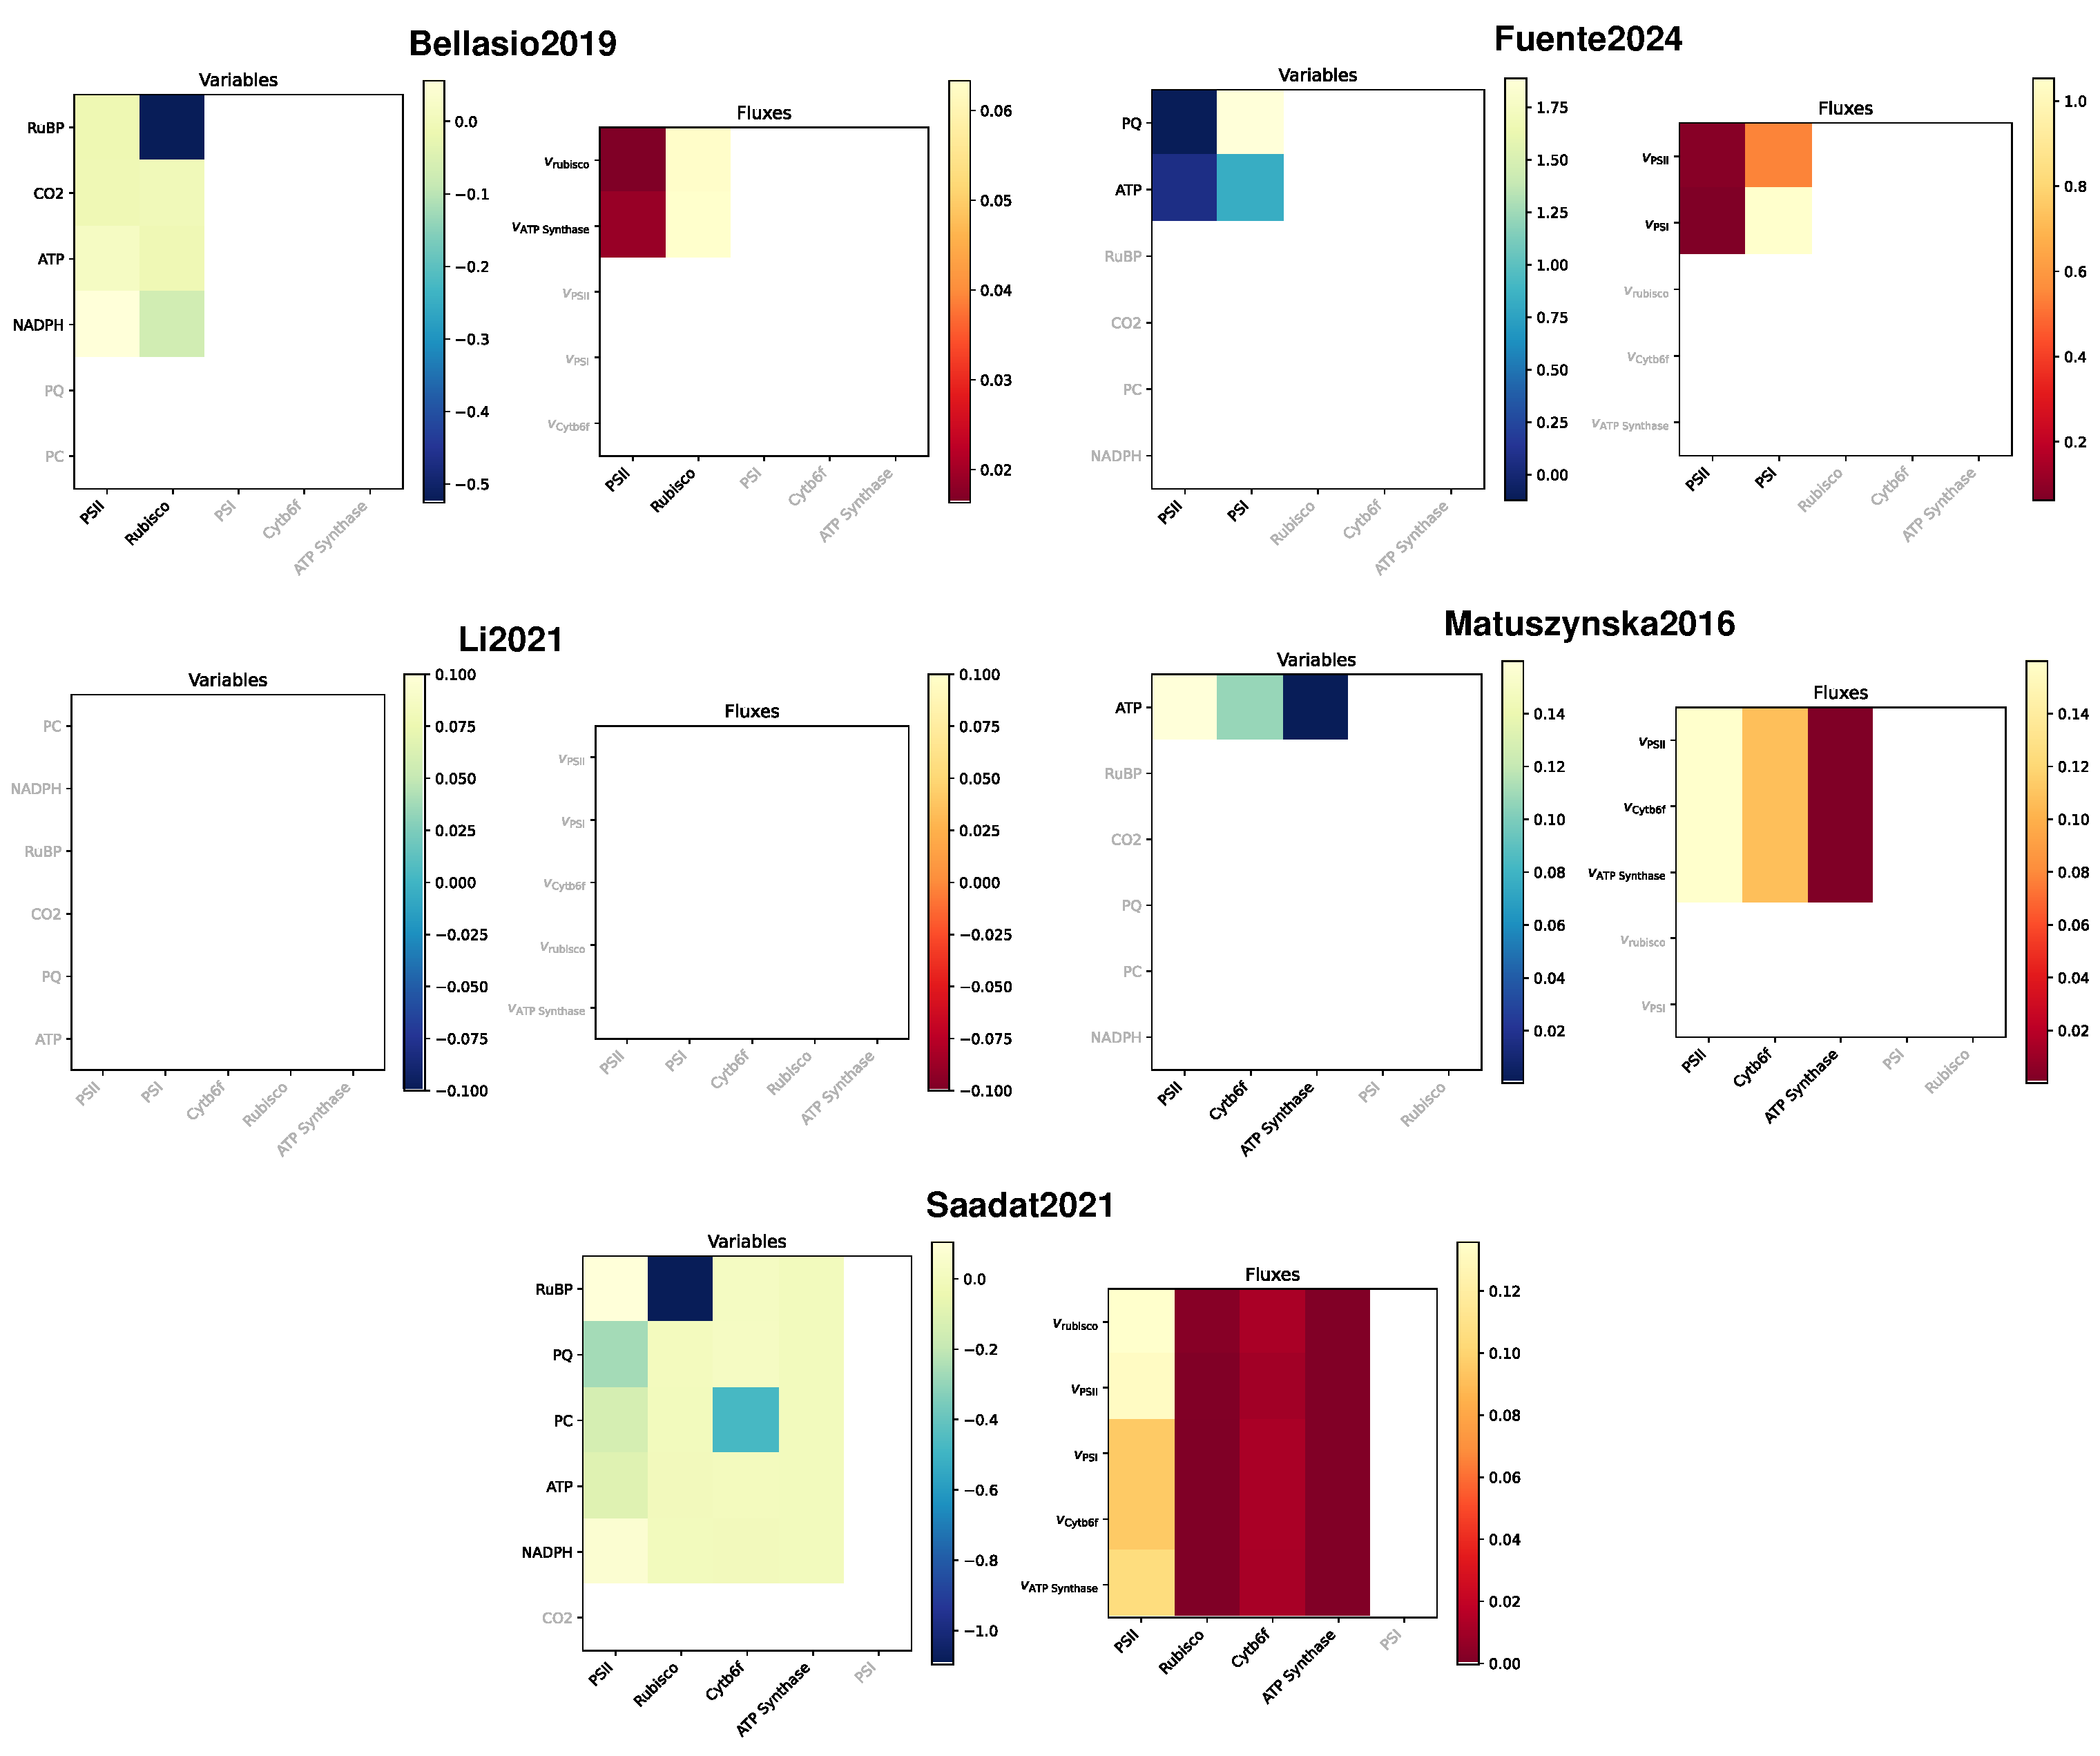
\includegraphics[width=0.7\textwidth]{Figures/Demonstrations/mca.pdf}
    \captionprof{Combined MCA of Photosynthesis demonstrations of all models.}{A sample \glsentryfull{mca} of typical photosynthesis variables and fluxes. A control coefficient analysis is to be performed, therefore each parameter represents a single coefficient of the photosynthesis rate. The rates chosen should represent \glsentryfull{vc}, \glsentryfull{vpsii}, \glsentryfull{vpsi}, \glsentryfull{vb6f} and \glsentryfull{vatp}. The variables chosen should represent \glsentryfull{co2} concentration, \glsentryfull{rubp}, \glsentryfull{pq_ox}, \glsentryfull{pc_ox}, \glsentryfull{atp}, and \glsentryfull{nadph}. For each parameter to be scanned, the model is simulated to steady-state, with a displacement of $\pm 0.01\%$ of each respective parameter. The control coefficients are then calculated for each variable and flux by the following formula: $C_{{p}}^{{x}} = \frac{{x_\mathrm{{upper}} - x_\mathrm{{lower}}}}{{2 \cdot \mathrm{{disp}} \cdot p}}$, where $C_{{p}}^{{x}}$ is the control coefficient of parameter $p$ on variable or flux $x$, and $\mathrm{{disp}}$ is the displacement value. $x_\mathrm{{upper}}$ and $x_\mathrm{{lower}}$ are the steady-state result of $x$ at either $+\mathrm{{disp}}$ and $-\mathrm{{disp}}$ respectively. It has to be noted that the \glsentryshort{mca} results can be very dependent on the other values of the parameters in the model, therefore the results shown here are only representative of the default parameter set of the model.}
    \label{fig:mca-demon}
\end{figure}

\subsubsection{Fitting of NPQ}

Of all models, only the Bellasio2019 could not produce a fit~\figref{fig:fit-demon}, due to it not having a quantity for \gls{F} nor \gls{npq}. Additionally, as the Li2021 model does not have quantity for \gls{F}, only the \gls{npq} curve could be plotted. However, the fitting could still occur, which produced a curve that followed the experimental data in lower light (\qty{90}{\micro\mol\per\square\meter\per\second}) and dark light (\qty{40}{\micro\mol\per\square\meter\per\second}) very closely. However, in high light (\qty{903}{\micro\mol\per\square\meter\per\second}), the curve first overfits and then underfits the data, showing an \gls{npq} curve that shows a peak before getting to a stable value.

The three other models, all show both a curve of \gls{F} and \gls{npq}, but have varying results. The Fuente2024 model shows a very close fit to the experimental data on the \gls{npq} side, but not on the \gls{F} side, where both the base \gls{F} and \gls{Fm} values are repeatedly higher. The model could best fit the \gls{npq} at high light and then first overfits but then underfits during lower light. At dark light, the \gls{npq} consistently overfit. For this model, the parameters that were fitted were \gls{npqmax} and \gls{k4}, by \qty{+80.44}{\percent} and \qty{-19.56}{\percent} respectively.

The Matuszynska2016 model shows a very similar fit to \gls{npq} as the Fuente2024 model, but is strikingly better at fitting the \gls{F} values. At high light, the \gls{F} and \gls{Fm} seem to be spot on, while following a very similar curve during lower light. There the points do not fit perfectly, but show a much nearer fit. In the last dark period, the base \gls{F} values are very close to the experimental data, while the fitted \gls{Fm} do not show the same rise from the prior period. For this model, the parameters fitted were \gls{gamma0}, \gls{gamma1}, \gls{gamma2}, \gls{gamma3}, and \gls{kzsat}, by \qty{22.12}{\percent}, \qty{573.61}{\percent}, \qty{259.39}{\percent}, \qty{1035.28}{\percent}, and \qty{4288.27}{\percent} respectively.

The Saadat2021 model shows a good fit for the \gls{F} and \gls{Fm} values, however the \gls{npq} is largely underfit during the high and lower light period. The dark period is also overfit, showing a much higher \gls{npq} than the experimental data. For this model, the parameters fitted were \gls{kphsat}, \gls{gamma0}, and \gls{kphsatlhc}, with \qty{-14.27}{\percent}, \qty{-99.99}{\percent}, and \qty{-16.89}{\percent} respectively.

\begin{figure}
    \centering
    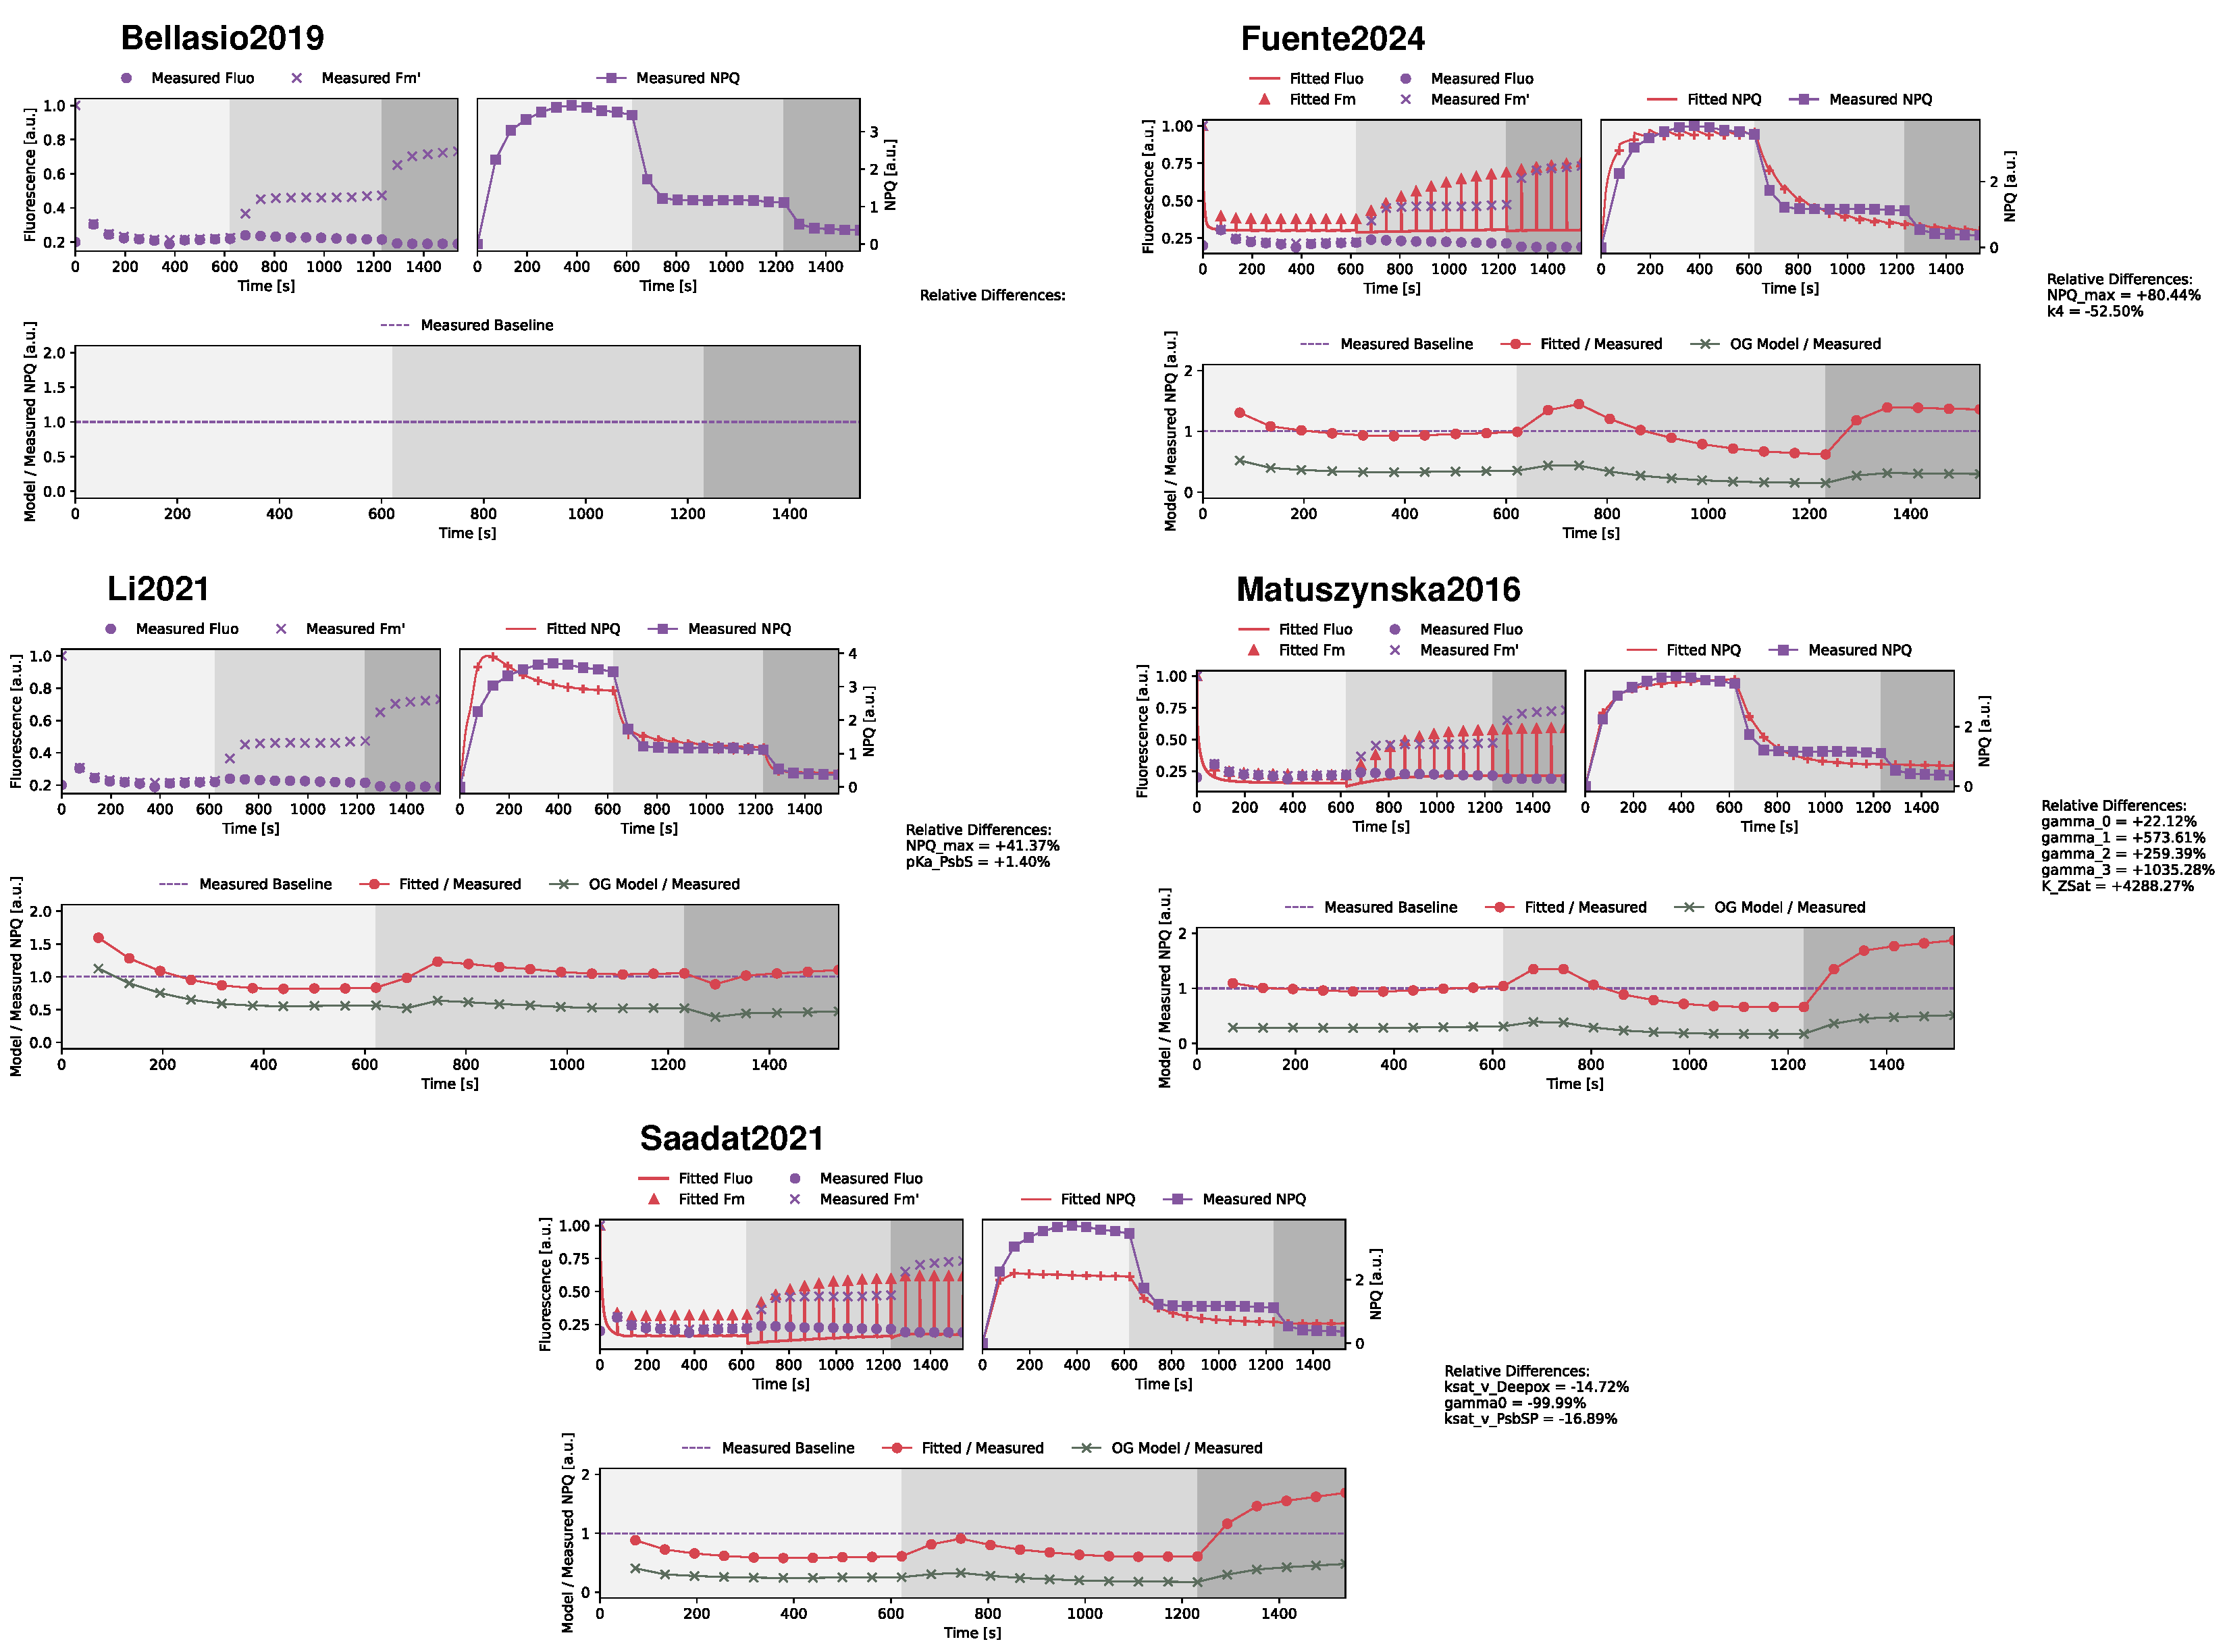
\includegraphics[width=\textwidth]{Figures/Demonstrations/fitting.pdf}
    \captionprof{Combined Fitting of NPQ demonstrations of all models.}{Sample fitting to experimental \glsentryfull{npq} data. The \glsentryshort{npq} data used is taken from experimental work published in von Bismarck (2022)~\cite{vonbismarckLightAcclimationInteracts2023} and was acquired using Maxi Imaging-PAM (Walz, Germany) using Col-0 \glsentryfull{arabidopsis} plants. It is assumed that the experiment follows the default \glsentryshort{pam} protocol of the machine, as no other experimental protocol has been given. Therefore, the protocol of each simulation follows the data given, where the length of one saturating pulse is set to \qty{720}{\micro\second} at a light intensity of \qty{5000}{\micro\mol\per\square\meter\per\second}. The light protocol consists of a dark adaptation period of 30 minutes to acclimate the simulation conditions. Then the actual protocol starts with a longer phase of high actinic light (\qty{903}{\micro\mol\per\square\meter\per\second}) for approximately 10 minutes, followed by a lower actinic light of (\qty{90}{\micro\mol\per\square\meter\per\second}) for 10 minutes, and then 5 minutes of a dark period. During each phase, saturating pulses are given approximately every 60 seconds. As the experimental data also provides exact time points for each pulse, these were taken as reference for the protocol and not the general time intervals. In the experimental work, the dark period consists of actual darkness, whereas in the simulation a low light intensity of \qty{40}{\micro\mol\per\square\meter\per\second} is used to avoid numerical issues. The fitting is performed using the \texttt{lmfit} package in Python with the leastsquare method. On top of that, a standard scaling towards the experimental data is done, to keep the fitting results in the same order of magnitude. To help the fitting converge, weights are applied to the data points, which are defined as the reciprocal of the standard deviation. These settings set are not to be taken as set in stone, as fitting is a highly experimental process and differing settings might be required depending on the model and data used. These settings are a basic starting point for fitting data to a model. The hardest and most impactful decision while fitting is the choice of parameters to fit. There are many ways to find which parameters may be most impactful to fit, such as sensitivity analysis or metabolic control analysis. However, either way experimenting with different parameter sets is always required to find the best fitting practice, which differs for each model and also data to fit to.}
    \label{fig:fit-demon}
\end{figure}

\subsection{Website}

When arriving on the \greensloth{} website, the user is first greeted with the Logo and the motto of the project, "Photosynthesis Models at your Pace"~\figref{fig:website-landingpage}. At the top of the page is a navigation bar, where the user can click to access different pages of the site. These are "Home", "Models", "GreenSloth" with a GitHub logo, "Compare", "How to Use", "About Us", and "Impressum". The "Home" page is the landing page of the website, that continues with an arrow pointing down to find out more. This brings the user to a section that explains the motivation of the project briefly, and then to another section that explains how to use the site. This section is also accessed by the "How To Use" navigation link in the top navigation bar and is separated into the three main aspects that \greensloth{} tries to provide: "Search", "Summary", and "Comparison"~\figref{fig:website-landingpage}. The "Search" part explains how the website's structure allows users to easily find models of photosynthesis, without the need of doing an intensive literature search. The "Summary" part explains how each model was prepared for \greensloth{}, including the detailed presentation of the model, the validation of the model, and the demonstrations performed. The "Compare" part explains how a direct comparison between models is made possible on the website. The user can however go one step further down, to a schematic overview of the photosynthetic machinery, where the user can click on different components that directly brings them to the "Models" page with the clicked machinery as a tag pre-selected.

\begin{figure}
    \centering
    \includegraphics[width=0.7\textwidth]{Figures/Website/landingpage.png}
    \captionprof{Screenshot of the landing page of the \greensloth{} website.}{A screenshot was done of the landing page of the \greensloth{} website, in a full screen mode. The top includes a navigation bar with links to the different pages of the website, and the main section includes the logo and motto of the project.}
    \label{fig:website-landingpage}
\end{figure}

\begin{figure}
    \centering
    \includegraphics[width=0.7\textwidth]{Figures/Website/howtouse.png}
    \captionprof{Screenshot of the How To Use page of the \greensloth{} website.}{A screenshot was done of the How To Use page of the \greensloth{} website, in a full screen mode. The top includes a navigation bar with links to the different pages of the website, and the main section includes three buttons, "Search", "Summary", and "Compare". They all independently show a section of text explaining the respective aspect of the website. These three aspects represent the three main aspect of model searching, understanding, and comparing that \greensloth{} tries to provide.}
    \label{fig:website-howtouse}
\end{figure}

\begin{figure}
    \centering
    \includegraphics[width=0.4\textwidth]{Figures/Website/machienry.png} \hspace{0.1\textwidth} \includegraphics[width=0.4\textwidth]{Figures/Website/machinery-select.png}
    \captionprof{Screenshot of the Machinery page of the \greensloth{} website.}{A screenshot was done of the page showing the photosynthesis machinery of the \greensloth{} website, in a full screen mode. The top includes a navigation bar with links to the different pages of the website, and the main section includes a schematic overview of the photosynthetic machinery, where the user can click on different components that directly brings them to the "Models" page with the clicked machinery as a tag pre-selected. On the left is the full schematic, while on the right is the representation, when the user hovers over one part of the machinery, in this case the "PSII" part. The hovering causes the all other parts to lose their color.}
    \label{fig:website-machienry}
\end{figure}

The "Models" page includes a search bar at the top, where the user can search for models solely by their name. Additionally, next to the bar is a button that opens the tag selection box. This allows the user to list all the models that have a specific tag, which can be related to the photosynthetic machinery, the demonstrations that can be performed with the model, or more~\figref{fig:website-howtouse}. The models are presented row by row, with their name and schemes for the easiest recognition. The user can click on the name of a model and be brought to that model's page.

\begin{figure}
    \centering
    \includegraphics[width=0.7\textwidth]{Figures/Website/modelpage.png}
    \captionprof{Screenshot of the Models page of the \greensloth{} website.}{A screenshot was done of the Models page of the \greensloth{} website, in a full screen mode. The top includes a navigation bar with links to the different pages of the website, and the main section includes a list of models that are available in the database. The list can be filtered by tags that are selected in the tag selection box.}
    \label{fig:website-modelpage}
\end{figure}

After choosing a model, the user is brought onto a page dedicated to that specific model~\figref{fig:website-model-top}. This page includes a sidebar on the left, which enables an easier navigation through the different sections of the page, which are "Summary", "ODE System", "Derived Quantities", "Parameters", "Derived Parameters", "Rates", "Figures", and "Demonstrations". At the top of the page, the name of the model is shown, along with the respective DOI as a link. Below that are two buttons, one to directly bring the user to the GitHub repository of that specific model, with a last update date, and another button that brings the user to the compare page, with this specific model already chosen. Briefly after these buttons, the summary section starts, with the scheme of the model on the left and a brief overview on what the model entails and how the implementation was done on the right. After that section, all the information of the model is shown in a table format, with the respective mathematical equations shown in a \LaTeX format. At the end, the figures and demonstrations sections showcase the recreations of the publication figures and the demonstrations that were performed, with a brief description. Each of the figures and demonstrations are in a collapsable box, to avoid overwhelming the user with too much information at once. If the user whishes to see details compared between the different models, they can click on the "Compare" in the sidebar or the top of the model page, which brings them to the compare page with the model already chosen.

\begin{figure}
    \centering
    \includegraphics[width=0.7\textwidth]{Figures/Website/model-top.png}
    \captionprof{Screenshot of a model page of the \greensloth{} website.}{A screenshot was done of the Fuente2024 model page of the \greensloth{} website, in a full screen mode. The top includes a navigation bar with links to the different pages of the website, and the main section includes a sidebar to navigate that specific page on the left and each section, one after another on the right. These sections are: "Summary", "ODE System", "Derived Quantities", "Parameters", "Derived Parameters", "Rates", "Figures", and "Demonstrations".}
    \label{fig:website-model-top}
\end{figure}

Arrived at the compare page, the user can choose two models from a dropdown menu and compare them side by side in five different categories. The first is the "Variables" category, that shows a Venn diagram of all the variables included in the models~\figref{fig:website-compare-var}. This Venn diagram is supposed to highlight in which variables the models overlap, but due to design and space issues, a figurative diagram is shown in the middle, with the actual variables listed to the left, right, or under it. The variables on the left are unique to the model on the left, and the same goes for the variables on the right, of course to the right sided chosen model. The variables underneath are all the variables, both models have in common. These are clickable, and when clicked, brings the user to the next category, the "Simulation".

\begin{figure}
    \centering
    \includegraphics[width=0.7\textwidth]{Figures/Website/compare-var.png}
    \captionprof{Screenshot of the compare page of the \greensloth{} website, with the variables category selected.}{A screenshot was done of the compare page of the \greensloth{} website, in a full screen mode. The top includes a navigation bar with links to the different pages of the website, and the main section includes two select boxes to choose the models to compare, and five different buttons that represent different categories to compare. The "Variables" category is selected, which shows a Venn diagram of all the variables included in the models. The variables on the left are unique to the model on the left, and the same goes for the variables on the right, of course to the right sided chosen model. The variables underneath are all the variables, both models have in common.}
    \label{fig:website-compare-var}
\end{figure}

In this category, the user can choose an overlapping variable between both models, and see a simple simulation over time~\figref{fig:website-compare-sim}. The protocol used always starts with a period of \qty{50}{\micro\mol\per\square\meter\per\second} light intensity for 10 seconds, followed by \qty{50}{\second} of light. This category also includes a slider, that lets the user change the light intensity of the light phase, giving a dynamic and instant way to showcase a simple simulation of the models. It has to be noted, that these simulations are not done live on the website, but have been pre-simulated for each of the models, and only the results are shown on the website. If the user, whishes to get more information on the models themselves, they can click on the "Information" tab, which brings them to a side by side numeric table view of all the meta-information of the models, such as the number of variables, parameters, and more.

\begin{figure}
    \centering
    \includegraphics[width=0.7\textwidth]{Figures/Website/compare-sim.png}
    \captionprof{Screenshot of the compare page of the \greensloth{} website, with the simulation category selected.}{A screenshot was done of the compare page of the \greensloth{} website, in a full screen mode. The top includes a navigation bar with links to the different pages of the website, and the main section includes two select boxes to choose the models to compare, and five different buttons that represent different categories to compare. The "Simulation" category is selected, which shows a simple simulation over time of an overlapping variable between both models. Here, the results of \glsentryfull{pq_ox} from the simulation of the Saadat2021 and the Fuente2024 at a \glsentryfull{ppfd} of \qty{100}{\micro\mol\per\square\meter\per\second} are shown.}
    \label{fig:website-compare-sim}
\end{figure}

The penultimate category is that of the "Demonstrations", where the user is able to choose from the demonstrations performed on the models, and see the results side by side~\figref{fig:website-compare-demon}. From the representing figure at the top, to the brief description underneath it. Then, the last category, "Schemes", is where both models' schemes are shown side by side, to easily compare the structure of the models~\figref{fig:website-compare-schemes}.

\begin{figure}
    \centering
    \includegraphics[width=0.7\textwidth]{Figures/Website/compare-demon.png}
    \captionprof{Screenshot of the compare page of the \greensloth{} website, with the demonstrations category selected.}{A screenshot was done of the compare page of the \greensloth{} website, in a full screen mode. The top includes a navigation bar with links to the different pages of the website, and the main section includes two select boxes to choose the models to compare, and five different buttons that represent different categories to compare. The "Demonstrations" category is selected, which shows two other select boxes, which contain the five possible demonstrations that were performed on each model. The Li2021 model on the left shows the PAM simulation, while the Matuszynska2016 model on the right shows the Day Simulation. The respective figures of the demonstrations are shown at the top, with a brief description of the demonstration underneath.}
    \label{fig:website-compare-demon}
\end{figure}

\begin{figure}
    \centering
    \includegraphics[width=0.7\textwidth]{Figures/Website/compare-schemes.png}
    \captionprof{Screenshot of the compare page of the \greensloth{} website, with the schemes category selected.}{A screenshot was done of the compare page of the \greensloth{} website, in a full screen mode. The top includes a navigation bar with links to the different pages of the website, and the main section includes two select boxes to choose the models to compare, and five different buttons that represent different categories to compare. The "Schemes" category is selected, which shows both models' schemes side by side. On the left, the Fuente2024 model is shown, while on the right, the Li2021 model is shown.}
    \label{fig:website-compare-schemes}
\end{figure}

The last two pages, "About Us" and "Impressum", include either information about the project and the team behind it, or legal information about the project. This, wraps up the entire \greensloth{} Website, and can be found here: \url{https://greensloth.rwth-aachen.de/}.

\newpage

\section{Discussion}

\subsection{Model Validations}

\subsubsection{Bellasio2019}

\subsubsection{Fuente2024}

\subsubsection{Li2021}

\subsubsection{Matuszynska2016}

\subsubsection{Saadat2021}

\subsection{Model Demonstrations}

\subsection{Website}

As the internet is now an integral part of most societies in the world, every person knows how to use a website. It keeps it simple and accessible for everyone, as it only needs an active internet connection to be accessed. On top of that, it is a quick way to convey information over the world, as direct sharing of a website can be done so, by a link. However, it is vital to give a website a good design, one that is curated to the target audience. This ensures the best way to convey the information it intends to. The advantages of a website are clear, accessibility, ease of use, and quick sharing. Advantages that support the goal of \greensloth{}.

The website created for \greensloth{} is designed to be as simple as possible, with a clear structure and easy navigation. It follows a modern and common style to convey its message, while separating key aspects of the work with models into different parts. The lists of implemented models and the ability to search for models by custom tags, can help the user in pinpointing their scope on which model they wish to look at. This would alleviate the problem of having to do an extensive literature search to find a model

\newpage

\pagenumbering{roman}
\setcounter{page}{\arabic{romannumbers} + 1}

\addcontentsline{toc}{section}{References}
\printbibliography

\end{document}
